% Rigorous certificates for open MINLPLib instances and an audit of listed
% dual bounds. The supplementary material is supplement.tex. Build both
% documents with `make` (development/build.md; output in build/).
\documentclass[11pt]{article}

% preamble.tex -- packages and macros shared by main.tex and supplement.tex.
% Each document inputs this file right after \documentclass and then names
% the other document with \externaldocument (xr-hyper), so that \cref works
% across the two PDFs. Build both with `make` (see development/build.md).

\usepackage[T1]{fontenc}
\usepackage{lmodern}
\usepackage[a4paper,margin=25mm]{geometry}
\usepackage{amsmath,amssymb,amsthm,mathtools}
\usepackage{booktabs,longtable,array}
\usepackage{rotating}
\usepackage{graphicx}
\usepackage[dvipsnames]{xcolor}
\usepackage[most]{tcolorbox}
\usepackage{microtype}
\usepackage[round]{natbib}
\usepackage{xurl}
\usepackage{xr-hyper}  % must come before hyperref
\usepackage[colorlinks=true,linkcolor=blue!50!black,citecolor=green!35!black,
            urlcolor=blue!50!black,filecolor=blue!50!black,  % filecolor: links to the other PDF
            bookmarksnumbered=true]{hyperref}
\usepackage[capitalise,noabbrev,nameinlink]{cleveref}

% xr-hyper appends the other document's file name to every imported label,
% also to cleveref's records (label@cref), so \cref would print
% "Section S3supplement.pdf". Read only the first field of these records.
% (\cpageref is not patched; do not use it across documents.)
\makeatletter
\def\cref@getref#1#2{%
  \expandafter\let\expandafter#2\csname r@#1@cref\endcsname
  \expandafter\expandafter\expandafter\def
    \expandafter\expandafter\expandafter#2%
    \expandafter\expandafter\expandafter{%
      \expandafter\paper@firstfield#2{}{}\@nil}}
\def\paper@firstfield#1#2#3\@nil{#1}
\makeatother

\graphicspath{{figures/}}
\setlength{\emergencystretch}{1em}  % avoids small overfull lines
% macros.tex -- notation, environments and helpers for the paper and its
% supplement. Loaded by preamble.tex after all packages (cleveref must
% already be loaded, so that theorem-like environments with a shared counter
% keep their own reference names). See development/labels.md for usage notes.

% ---------------------------------------------------------------------------
% Theorem-like environments: one counter, numbered within sections
% (Theorem 4.6, Lemma 4.1, ...; in the appendices A.1, B.2, ...; in the
% supplement S1.3, S5.1, ...).
% ---------------------------------------------------------------------------
\theoremstyle{plain}
\newtheorem{theorem}{Theorem}[section]
\newtheorem{lemma}[theorem]{Lemma}
\newtheorem{proposition}[theorem]{Proposition}
\newtheorem{corollary}[theorem]{Corollary}
\theoremstyle{definition}
\newtheorem{definition}[theorem]{Definition}
\newtheorem{assumption}[theorem]{Assumption}
\theoremstyle{remark}
\newtheorem{remark}[theorem]{Remark}
\newtheorem{observation}[theorem]{Observation}

% Hypotheses with a fixed tag instead of a number, e.g. (H) and (H0):
%   \begin{hypothesis}{H}[display]  ...  \end{hypothesis}
% prints "Hypothesis H (display)."; \cref gives "Hypothesis H".
\theoremstyle{definition}
\newtheorem{hypothesisinner}{Hypothesis}
\NewDocumentEnvironment{hypothesis}{m o}
  {\renewcommand{\thehypothesisinner}{#1}%
   \IfValueTF{#2}{\hypothesisinner[#2]}{\hypothesisinner}}
  {\endhypothesisinner}
\theoremstyle{plain}

\crefname{theorem}{Theorem}{Theorems}
\crefname{lemma}{Lemma}{Lemmas}
\crefname{proposition}{Proposition}{Propositions}
\crefname{corollary}{Corollary}{Corollaries}
\crefname{definition}{Definition}{Definitions}
\crefname{assumption}{Assumption}{Assumptions}
\crefname{remark}{Remark}{Remarks}
\crefname{observation}{Observation}{Observations}
\crefname{hypothesisinner}{Hypothesis}{Hypotheses}

% ---------------------------------------------------------------------------
% Boxes
% ---------------------------------------------------------------------------
% Certificate box (one per theorem; fields listed in development/labels.md):
%   \begin{certbox}[Certificate for \cref{thm:lnts-opt}]
%     \certitem{Inputs}{...}
%     ...
%   \end{certbox}
\newtcolorbox{certbox}[1][Certificate]{%
  breakable, enhanced jigsaw, colback=black!3, colframe=black!55,
  boxrule=0.5pt, arc=1pt, left=6pt, right=6pt, top=4pt, bottom=4pt,
  fonttitle=\small\bfseries, coltitle=black, colbacktitle=black!12,
  title={#1}, fontupper=\small}
\newcommand{\certitem}[2]{\par\noindent\hangindent=1.5em\textsf{#1:}\enspace #2\par}

% Numbered text box ("Box 1"), e.g. results at a glance, the camshape800
% example, the SCIP defect:
%   \begin{infobox}[label={box:glance}]{Results at a glance} ... \end{infobox}
\newtcolorbox[auto counter, crefname={Box}{Boxes}]{infobox}[2][]{%
  breakable, enhanced jigsaw, colback=blue!3, colframe=blue!40!black,
  boxrule=0.5pt, arc=1pt, left=6pt, right=6pt, top=4pt, bottom=4pt,
  fonttitle=\small\bfseries, coltitle=black, colbacktitle=blue!10,
  title={Box~\thetcbcounter: #2}, fontupper=\small, #1}

% ---------------------------------------------------------------------------
% Instance names: \inst{waterno2_06} sets the MINLPLib name in typewriter
% type; underscores need no escaping. Line breaks are allowed only after
% an underscore or a hyphen (xurl's break-anywhere rule is switched off).
% The name is always upright: in italic text (theorem statements) the slanted
% typewriter font left a visible gap after each underscore.
% ---------------------------------------------------------------------------
\DeclareUrlCommand\instname{\def\UrlFont{\ttfamily\upshape}%
  \def\UrlBreaks{\do\_\do\-}\def\UrlBigBreaks{}\def\UrlNoBreaks{}%
  \Urlmuskip=0mu\relax}
\DeclareRobustCommand{\inst}{\instname}
\pdfstringdefDisableCommands{\def\inst#1{\detokenize{#1}}}

% ---------------------------------------------------------------------------
% Notation (development/outline.md, section 4)
% ---------------------------------------------------------------------------
% Model, feasible set, optimal value
\newcommand{\model}{\mathcal{M}}                  % stored OSIL model M (M_I: \model_I)
\newcommand{\feas}[1][\model]{\mathcal{F}(#1)}    % exactly feasible set F(M)
\newcommand{\vstar}{v^{*}}                        % optimal value: \vstar(\model)
% Certified bound, primal value, gaps, sense
\newcommand{\Lcert}{L}                            % certified (valid) dual bound
\newcommand{\Uprim}{U}                            % upper end of the objective enclosure at an exactly feasible point
\newcommand{\gapabs}{\Delta}                      % absolute gap s(U - L)
\newcommand{\gaprel}{\delta}                      % relative gap Delta / min(|L|,|U|)
\newcommand{\sense}{s}                            % +1 minimize, -1 maximize
% Data readings (a) GAMS text, (b) OSIL text [all claims], (c) binary64 data
\newcommand{\reading}[1]{reading~(#1)}
% Arithmetic tags [E] exact, [I] mpmath interval, [F] own outward-rounded binary64, [L] library hypothesis
\newcommand{\arith}[1]{\textsf{[#1]}}
% Evidence levels \evid{hand}, \evid{stored}, \evid{rerun} (development/terminology.md) and
% trust-base terms T-int, T-fp, T-mp, T-read, T-code, T-thm
\newcommand{\evid}[1]{\textsf{#1}}
\newcommand{\trust}[1]{\textsf{T-#1}}
% Floating point and listing strings
\newcommand{\fl}{\operatorname{fl}}               % round-to-nearest binary64
\newcommand{\uround}{\mathbf{u}}                  % unit roundoff 2^{-53}
\newcommand{\dunit}[1]{u(#1)}                     % unit of the last displayed digit of string #1
\newcommand{\dval}[1]{d(#1)}                      % rational value of the decimal string #1
% KAN objects: network relaxation R and OSIL model without partition-of-unity rows R_P
\newcommand{\Rnet}{\mathcal{R}}
\newcommand{\RP}{\mathcal{R}_{\mathrm{P}}}
% Number sets and operators
\newcommand{\R}{\mathbb{R}}
\newcommand{\Q}{\mathbb{Q}}
\newcommand{\Z}{\mathbb{Z}}
\newcommand{\N}{\mathbb{N}}
\DeclareMathOperator{\proj}{proj}
\DeclareMathOperator{\dist}{dist}
\DeclareMathOperator*{\argmin}{arg\,min}
\DeclareMathOperator*{\argmax}{arg\,max}
% Scientific notation in text or math: \sci{3.1}{-9} -> 3.1 x 10^-9
\newcommand{\sci}[2]{\ensuremath{#1\cdot 10^{#2}}}

% ---------------------------------------------------------------------------
% Placeholders (each use also writes a warning to the log)
% ---------------------------------------------------------------------------
\definecolor{todocolor}{rgb}{0.8,0,0}
\DeclareRobustCommand{\TODO}[1]{%
  \textcolor{todocolor}{\textbf{[TODO: #1]}}%
  \GenericWarning{}{LaTeX Warning: TODO: #1}}
\DeclareRobustCommand{\archiveDOI}{%
  \textcolor{todocolor}{\texttt{[archive DOI]}}%
  \GenericWarning{}{LaTeX Warning: archive DOI placeholder}}



% Labels of the supplement (Section S1, Theorem S1.2, ...). Its .aux file
% is in build/; links open supplement.pdf next to main.pdf. The supplement
% has its own bibliography, so its citations are not imported.
\externaldocument[][nocite]{build/supplement}[supplement.pdf]

\title{Rigorous certificates for open MINLPLib instances\\
  and an audit of listed dual bounds}
\author{}
\date{}

\begin{document}
\maketitle

% Abstract (at most 250 words). Plan: development/outline.md, section 2,
% updated with the numbers in data/numbers.json. The AI-use disclosure is in
% Section 2.6 and in the declarations, not here.
% Round 3 (sol-referee 1, opus-writing 21): the 79 solver bounds are described as
% bounds on unmodified non-KAN GAMS files, with the sampled GAMS/OSIL correspondence
% stated as an assumption; the abstract is one word shorter than the round-2
% version (250 words in the source, macros and inline math counted as one word).
\begin{abstract}
MINLPLib lists tolerance-feasible points and solver-reported dual bounds and marks an instance solved when three solvers claim global optimality; none of these is a proof.
We study 43 nonconvex instances without this mark, reading decimals as rationals and requiring exact feasibility.
For 31 instances we prove a dual bound and exhibit an exactly feasible point within a relative gap of at most \sci{3.1}{-9}; for nine we prove exact optima, and for seven of the 31, floating-point closures or near-closures (one for a copy) had been reported.
For five pump-scheduling instances we raise the best listed dual bounds 1.68- to 6.21-fold (gaps at most 10.82\%); for \inst{ann_cumene_tanh}, whose variant \inst{ann_cumene_exp} has floating-point closures, we prove a bound with gap 0.195\%.
Our six Kolmogorov--Arnold network (KAN) instances have no exactly feasible point; dropping their partition-of-unity rows, we enclose the optima within \sci{2.42}{-8}.
Certificates combine classical devices (Lagrangian duality, Sturm comparison, Taylor models) with exact or outward-rounded arithmetic; with named exceptions, separately written code rechecks them, sometimes only for a weaker bound or part of the domain.
Of MINLPLib's 11,086 per-solver dual bounds, we prove 22 invalid under a stated display hypothesis; four proved relative margins exceed 1\% and eleven are below $10^{-6}$.
A seed-dependent SCIP~10 error gives wrong optimal values on \inst{waterno2} subproblems.
All 79 one-hour BARON, Gurobi and SCIP dual bounds with globality guarantees for unmodified non-KAN GAMS files were weaker than ours, assuming GAMS--OSIL agreement where only sampled; BARON reached two tolerance-level closures.
Code, certificates and points are archived.
\end{abstract}

\noindent\textbf{Keywords:} global optimization; mixed-integer nonlinear programming; benchmark libraries; MINLPLib; verified computation; interval arithmetic; exact rational arithmetic; dual bounds

\noindent\textbf{Mathematics Subject Classification (2020):} 90C26; 90C11, 90C30, 90C46, 65G20, 65G30


% Plan: development/outline.md, section 5, "§1 Introduction"; contributions
% and qualifiers in section 3. Numbers from data/numbers.json. Round-1
% revision: items G1-04 to G1-09 of development/reviews/round1/adjudication.md.
% Round-2 revision: items G1-10 to G1-14 of
% development/reviews/round2/adjudication.md. Round-3 revision: opus-writing 3,
% 5-8, sol-referee 1 and the optional lnts50 cut of opus-referee 8
% (development/reviews/round3/).
\section{Introduction}\label{sec:intro}

We examine 43 nonconvex instances of the mixed-integer nonlinear programming (MINLP) library MINLPLib \citep{bussieck2003-minlpliba-collection-of-test-models,vigerske2014-minlplib-2} that the library does not mark as solved, and ask what can be proved about them when the stored decimal data are read as rational numbers and feasibility is exact.
For 31 of them we prove a dual bound and exhibit an exactly feasible point within a relative gap of at most \sci{3.1}{-9}.
Applying the same standard to the library's records and to solver output, we prove 22 listed per-solver dual bounds invalid under a stated hypothesis on how MINLPLib's pages display numbers, and we report a seed-dependent error in SCIP~10 (\cref{sec:intro-contrib}).

\subsection{Benchmark records are not proofs}\label{sec:intro-records}

Benchmark libraries record what solvers have reported; they rarely record what has been proved.
MINLPLib, a standard benchmark library for MINLP solvers and methods, lists on its 1,633 instance pages solution points with their maximal absolute constraint violation, dual bounds reported by individual solvers, and solved marks \citep{vigerske2026-minlplib-documentation-database-snapshot-2026}.
The library adjusts the points so that integrality and variable bounds hold exactly, but algebraic rows may keep residuals; points whose violation lies below the feasibility tolerance define the best primal bound.
The dual bounds carry no proof.
In the words of the library's FAQ, they ``are just the best value as computed in some run with some option settings on some machine at some time in the past'' \citep{vigerske2026-minlplib-a-library-of-mixed}.
The solved mark, shown as the letter S on the instance pages, means that ``at least 3 solvers claim global optimality (up to a relative optimal tolerance (gap) of $10^{-6}$)'' for the best known point, or that at least three solvers claim infeasibility \citep{vigerske2026-minlplib-documentation-database-snapshot-2026}.
No formula for the gap is documented.
The solved mark is a consensus label, not a check.
When MINLPLib~2 was assembled, the maintainer noted ``No way to verify correctness of bound!'' \citep[slide 23, PDF p.~38]{vigerske2014-towards-minlplib-2-0}, and a reported bound was trusted when at least two other solvers confirmed it \citep[p.~140]{vigerske2014-minlplib-2}.

These records, and solver claims of the same kind, nevertheless serve as reference values.
The SCIP~8 study counts a run on a MINLPLib instance as failed when its bounds contradict the bounds on the MINLPLib page \citep[\S3.3, author manuscript p.~23]{bestuzheva2025-global-optimization-of-mixed-integer}.
A machine-learning approach to global optimization calls a result on a MINLPLib model optimal when its gap is below 0.1\%, while noting that its solutions may be infeasible \citep[pp.~24, 32]{bertsimas2025-towards-a-practical-global-optimization}.
The public CAMINO benchmark data record Gurobi bounds that equal the recorded objective values \citep{ghezzi2026-camino-benchmark-results-for-nonconvex}.
A study of optimization over trained Kolmogorov--Arnold networks (KANs) reports SCIP optima at zero gap \citep{karia2025-deterministic-global-optimization-over-trained}.
Uses that need only tolerance-level reference values are consistent with these records.
A conclusion about exact optimality is not: a gap measured against a listed point that is feasible only within a tolerance can compare a dual bound with a value below the optimum, and a reported bound can be invalid.
\Cref{box:camshape800} shows what the records of one instance say.

\begin{infobox}[label={box:camshape800}]{What the records of \inst{camshape800} say}
\inst{camshape800} is a discretized cam-design problem from the COPS collection \citep{dolan2004-benchmarking-optimization-software-with-cops-2}, with 1,599 continuous variables and 1,600 rows.
Its optimal value is a rational number $v_{800}$ with
\[
  -4.27427414195420 \;\le\; v_{800} \;\le\; -4.27427414195419,
\]
attained at an explicit rational point (\cref{thm:camshape-opt}).
The proof is a discrete comparison argument with exact rational checks.
MINLPLib's best listed dual bound, $-5.12584096$, is valid but lies more than 0.85 below $v_{800}$.
The best listed point, p2, has listed violation $3\cdot10^{-10}$: it violates 722 rows by more than $10^{-12}$, most of them by about $10^{-10}$.
Its objective lies at least \sci{3.27}{-5} below $v_{800}$, so no exactly feasible point attains it; it is a tolerance artifact (\cref{sec:semantics-categories}).
Under the library's rules p2 defines the best primal bound, so the gap between the listed bounds compares a valid but weak dual bound with a value below the optimum.
\end{infobox}

\subsection{Approach and main observations}\label{sec:intro-approach}

We take as the model of an instance its stored OSIL file, read every decimal string in it as the rational number it denotes, and call a point feasible only if it satisfies every row, bound and integrality requirement exactly (\cref{sec:semantics-model}).
A closure (a certified relative gap of at most $10^{-6}$, MINLPLib's tolerance; \cref{def:sem-certificate}) then needs two certificates: a dual bound that is valid for every exactly feasible point, and an exactly feasible point whose objective value is enclosed rigorously.
We built each dual bound from the structure of its model and evaluated it in exact rational or outward-rounded arithmetic.
Apart from named exceptions, separately written code rechecks every computer-assisted dual certificate, for some families only for a slightly weaker bound or, for \inst{eg_disc2_s}, only on part of the domain (\cref{sec:semantics-protocol} states how these implementations were produced and what ``separately written'' means).

Three observations stand out; we return to them in \cref{sec:conclusion}.
\begin{enumerate}
\item Once a bound fitted to the structure of the model was in place, 12 closures needed no branching and 15 more branched in at most three dimensions, among them the \inst{ex6_2_5} bound, with 131,111 two-dimensional boxes.
  The \inst{pindyck} certificate divides one box in $\R^{112}$ into 9 leaves, and the three \inst{eg} certificates branch on their 7 original variables, with up to 1,114,361 leaves.
  We do not test why general-purpose solvers did not find such bounds; \cref{sec:interpretation} offers an interpretation.
\item Fifteen closures exploit the stage structure of the model: eleven split the objective along the stages (\cref{lem:split-bound}), and the four \inst{catmix} certificates bound the value functions of a backward dynamic program (\cref{lem:split-minorant}); in both, every stage problem is small enough to be minimized rigorously (\cref{sec:split}).
\item Exact feasibility decides questions that tolerance-feasible data leave open.
  Some listed dual bounds are invalid under every feasibility tolerance, which an exactly feasible point proves (\cref{sec:audit}).
  Some listed and published optimal values hold only within tolerances.
  Along long chains of coupled rows, a tolerance can lower the objective by far more than its own size: on \inst{camshape}, points that violate each row and bound by at most $\varepsilon$ lie at most $0.61\,n^2\varepsilon$ below the optimum (proved for the values $\varepsilon\le10^{-8}$ of \cref{tab:camshape-deficit}), and explicit tolerance-feasible points reach about 87\% of this bound (numerical evidence).
  SCIP~10 returns wrong optimal values on some subproblems; in the 15 wrong runs that we traced, the error is triggered by the decimal identity $0.7^3=0.343$, which fails after rounding to binary64 (\cref{sec:solvers-invalid}).
\end{enumerate}

\subsection{Contributions}\label{sec:intro-contrib}

The certificates are built per instance; we implemented no general solver and claim no general solver capability.

\begin{description}
\item[C1 (certificates under exact semantics).]
For 31 instances that are not marked solved (snapshot of \cref{sec:semantics-model}) we prove a dual bound that is valid for every exactly feasible point of the stored OSIL model, and we exhibit an exactly feasible point within a relative gap of at most \sci{3.1}{-9} (\cref{tab:closures}).
They come from 14 instance families; 28 are continuous and three mixed-integer.
We chose the instances by judged tractability, so 31 is not a solve rate (\cref{sec:results-selection}).
For nine of them (\inst{camshape100}--\inst{camshape800}, \inst{hvycrash} and \inst{lnts50}--\inst{lnts400}) we characterize the optimal value exactly and prove that it is attained.
To our knowledge, within the search described in \cref{sec:intro-prior} and \cref{app:literature}, no rigorous certificate had been published for any of these 31 stored models.
For seven of them, floating-point closures or near-closures had been reported: for six on the same model, for \inst{dtoc5} on a copy under assumed variable bounds; \cref{sec:results-prior} credits these and the other earlier results by name.
For the five \inst{waterno2} instances we prove dual bounds 1.68 to 6.21 times the best listed ones, leaving relative gaps of at most 10.82\% (\cref{tab:unclosed}); we claim no priority for period decomposition.
For \inst{ann_cumene_tanh} we prove a dual bound within 0.195\% of an exactly feasible point; it also holds for \inst{ann_cumene_exp}, which writes $\tanh$ through $\exp$ and which SCIP and LINDO closed in floating point \citep{vigerske2026-minlplib-a-library-of-mixed}; our bound is weaker than their values.
The six KAN instances in our set have no exactly feasible point (\cref{prop:kan-infeasible}); for the model $\RP$ without their partition-of-unity rows and its network relaxation $\Rnet$ we enclose the optimal values (\cref{thm:kan-enclosure}); these enclosures say nothing about points that satisfy the OSIL rows only within a tolerance.

\item[C2 (audit of listed dual bounds).]
We screened all 11,086 per-solver dual bounds on MINLPLib's 1,633 instance pages against the 2,816 listed points.
Under a stated hypothesis on how the pages display numbers (\cref{hyp:audit-display}), we prove 22 listed bounds on 18 instances invalid: 19 on 15 instances from the screen, each proved again by a second implementation, and three LINDO bounds on \inst{rocket100}, \inst{rocket200} and \inst{rocket400} outside it.
Only \inst{rocket100} needs \cref{hyp:audit-display} itself; the other 21 refutations need only that each display arises from the reported number by decimal roundings or truncations (\cref{sec:audit-hyp}).
Four margins exceed 1\% of the displayed value and eleven lie below $10^{-6}$; no refutation contradicts a solved mark, and we attribute no cause.
To our knowledge, within the search of \cref{app:literature}, this is the first systematic screen of MINLPLib's listed per-solver bounds that refutes listed bounds only by proving that an exactly feasible point exists below them; earlier checks compared bounds with other solvers or with reference values (\cref{sec:intro-records,sec:intro-prior}).

\item[C3 (solver and published claims).]
SCIP 10.0.2, 10.0.3, 10.1.0 and a development snapshot \citep{hojny2025-the-scip-optimization-suite-10} return wrong optimal values on subproblems of \inst{waterno2_06} for some random seeds; exactly feasible rational witnesses, which SCIP~10.0.2's feasibility check accepts, refute these claims, and a reproducer with 15 variables shows the same error (\cref{sec:solvers-invalid}).
Assuming that CAMINO used the current MINLPLib files and recorded AMPL's \texttt{bestbound}, its bounds for Gurobi 13.0.0 on \inst{eg_disc2_s}, \inst{eg_disc_s} and \inst{eg_int_s} \citep{ghezzi2026-camino-benchmark-results-for-nonconvex} exceed the objective values of exactly feasible points by at least 4.33\%, 7.48\% and 80.5\%.
Assuming that the \texttt{.nl} file of QPLIB\_8803 encodes the MINLPLib model \inst{optcdeg2}, MINOTAUR~0.4.1's infeasibility report for it is contradicted by an exactly feasible point.
Both claims are invalid as recorded; the causes are unknown.
We also catalogue listed and published optimal values that no exactly feasible point attains (\cref{sec:solvers-tolerance}).
In one-hour runs of BARON 26.5.27, Gurobi 13.0.2 and SCIP 10.0.3 on the GAMS files of all 43 instances, all 79 final dual bounds with a globality guarantee for the unmodified models of the non-KAN instances are weaker than our certified bounds, and five final dual bounds improve the best listed dual bound.
Where \cref{tab:sem-gams} compares the GAMS and OSIL forms only at sample points, this comparison assumes that the two forms define the same model; elsewhere the forms are identical, except for \inst{catmix}, to whose GAMS form \cref{prop:catmix-transport} transfers our bounds.
\Cref{sec:solvers-campaign} discusses the 30 other finite bounds: values without a globality guarantee, bounds on models that SCIP modified, and values on the KAN instances, for which our bounds concern $\Rnet$.
Only BARON's runs on \inst{camshape100} and \inst{camshape200} ended with a relative gap of at most $10^{-6}$; they are tolerance-level closures (\cref{prop:baron-camshape}).
The runs check the status of current solvers on these instances; they do not rank them.

\item[C4 (reproducibility).]
The archive that accompanies this paper (\archiveDOI) holds the models with their SHA-256 hashes, the certificate data, the exact point definitions, and the first and the separately written implementations.
A number file gives the exact value, source and rounding direction of every generated certified display (bounds, primal ends, gaps and derived margins), and a claim register maps each result to its checkers and inputs.
Replay commands come in three tiers of effort (\cref{sec:repro,app:repro}); the archive separates replay of stored certificates from regeneration, which may produce a different valid certificate (\cref{sec:semantics-protocol}).
\end{description}

\subsection{Prior work and what is classical}\label{sec:intro-prior}

Other benchmark libraries check points against tolerances and compare solver results: MIPLIB uses arbitrary-precision solution checkers with explicit tolerances and removed numerically inconsistent instances \citep{koch2011-miplib-2010-mixed-integer-programming,gleixner2021-miplib-2017-data-driven-compilation}, and PAVER automates the analysis of benchmark data \citep{bussieck2014-paver-2-0-an-open}.
COPS, CUTE and CUTEst, QPLIB and the COCONUT collections record reference values and residuals with varying levels of checking \citep{dolan2004-benchmarking-optimization-software-with-cops-2,bongartz1995-cute-constrained-and-unconstrained-testing,gould2015-cutest-a-constrained-and-unconstrained,furini2018-qplib-a-library-of-quadratic,shcherbina2003-benchmarking-global-optimization-and-constraint}.
The benchmark records inspected in our search do not supply nonlinear dual-bound certificates that a user can check.

The closest precedent for certificates on MINLPLib is \citet{halbig2024-computing-optimality-certificates-for-convex}, who compute optimality certificates for 17 of 67 selected convex MINLPLib instances; their certificates rest on convexity, and all our instances are nonconvex.
Their computational construction and verification solve the auxiliary optimization problems with Gurobi; here we require exact or outward-rounded verification on the stored nonconvex models.
Wrong answers of global solvers are well documented.
\citet{neumaier2005-a-comparison-of-complete-global} record false global and infeasibility claims of complete solvers, and \citet{nowak2008-lago-a-heuristic-branch-and} report a wrong BARON root bound on \inst{bayes2_10}.
\citet{vigerske2017-scip-global-optimization-of-mixed} discard runs in which SCIP computed a wrong dual bound, and \citet{montanher2018-a-computational-study-of-global} and \citet{bestuzheva2025-global-optimization-of-mixed-integer} count wrong or inconsistent results in large studies.
Feasibility-tolerance artifacts in solver comparisons are a known concern among developers \citep[Berthold's contribution, \S3.6]{bonami2018-designing-and-implementing-algorithms-for}.
These studies decide conflicts by comparison with reference values or other solvers, not by exact feasibility.

Rigorous global optimization supplies the tools: interval branch and bound with existence tests \citep{kearfott2003-globsol-history-composition-and-advice,kearfott2011-interval-computations-rigour-and-non,neumaier2004-complete-search-in-continuous-global}, safe LP and SDP bounds by directed rounding \citep{neumaier2004-safe-bounds-in-linear-and,jansson2006-vsdp-verified-semidefinite-programming,jansson2007-rigorous-error-bounds-for-the}, rigorous search frameworks \citep{domes2009-gloptlab-a-configurable-framework-for}, and certified minima for difficult test functions \citep{vanaret2014-certified-global-minima-for-a}.
Current interval solvers such as IbexOpt combine reliable affine and Taylor relaxations and certify LP-derived lower bounds by interval post-processing \citep{araya2025-hybridizing-two-linear-relaxation-techniques}.
By default IbexOpt relaxes equality rows by a tolerance; in its rigor mode it returns a box that is proved to contain a point satisfying the equalities exactly \citep{ibex2026-ibexopt-ibex-documentation}.
We did not run such a solver, because this study builds instance-specific certificates rather than comparing methods; its lower bounds would be a natural rigorous baseline for ours, and whether they reach our bounds on these instances is open.
Exact rational LP and MIP solvers and checkable MIP certificates \citep{applegate2007-exact-solutions-to-linear-programming,cook2011-an-exact-rational-mixed-integer,cook2013-a-hybrid-branch-and-bound,cheung2017-verifying-integer-programming-results,eifler2023-a-computational-status-update-for} set the precedent, which we follow, of treating input data as rationals.
Recent work certifies propagation and dual proof analysis in an exact MIP solver \citep{borst2024-certified-constraint-propagation-and-dual}, builds VIPR certificates from black-box floating-point ILP solvers \citep{szeider2026-vipr-certificate-construction-from-black}, and analyses the numerical correctness of branch-and-bound decisions \citep{hoen2025-analyzing-the-numerical-correctness-of}; these certify or check linear MIP results, whereas our obligations are nonlinear and sometimes transcendental.
In recent MINLP work the global bound remains solver output: Xpress Global withholds a global-optimality claim when it imposes artificial bounds \citep{belotti2025-solving-minlps-to-global-optimality}, \citet{merx2026-from-computational-certification-to-exact} pairs a solver-reported $\varepsilon$-global bound with exactly recovered coordinates, and a closure of the seven-electron Thomson problem, a MINLPLib model family, rests on subproblems solved by a global solver \citep{kuznetsov2024-convexification-and-global-optimization-of}.

Every mechanism in our certificates is classical: Lagrangian decomposition, Krotov- and Mangasarian-type sufficiency and relaxed dynamic programming, LP formulations for polynomial optimization of bounded treewidth, discrete Sturm comparison, the Gibbs tangent-plane test, hidden convexity, SDP relaxations of optimal power flow, Taylor models, affine arithmetic and safe per-box LP bounds, interval existence tests and rational PSD certificates; \cref{app:literature-scope} gives the references.
What is new are the instance-specific constructions, their exact or outward-rounded evaluation on the stored models, and what they show about benchmark data and solver claims; the exact \inst{camshape} envelope, the scalar \inst{lnts} characterization and the curved \inst{optcdeg2} split are examples.
Our search for prior results covered the 43 instance names, their source models and copies, and the literature cited above, up to 2026-10-04.
It is a bounded search, not a proof of priority; \cref{app:literature} describes it and lists the sources we could not read.

\subsection{Organization}\label{sec:intro-org}

\Cref{sec:semantics} fixes the semantics and the verification protocol, \cref{sec:results} summarizes the results, \cref{sec:split,sec:other,sec:points} give the certificates and the exactly feasible points, \cref{sec:audit,sec:solvers} the audit and the solver and published claims, \cref{sec:interpretation} an interpretation and recommendations, and \cref{sec:repro,sec:conclusion} reproduction, limitations and conclusions.
\Cref{app:semantics,app:splitproofs} treat the reading of the models and the proofs for \cref{sec:split-framework}; the supplementary material, whose numbers carry the prefix~S, gives the certificates by family and all further details.

% Plan: development/outline.md, section 5, "§2"; conventions in section 4.
% Round-1 revision: items G1-01, G1-02 and G1-10 to G1-15 of
% development/reviews/round1/adjudication.md. Round-2 revision: items G1-01
% to G1-08 of development/reviews/round2/adjudication.md. Round-3 revision:
% opus-referee 2 and 3, opus-writing 2 and 9 (development/reviews/round3/).
% The pointer to tab:trust-full in Section 2.6 refers to the Table S37 column on
% whether the second session read the first code (opus-referee 2; families
% from the G1 session-record check in development/revise4-result.json; column
% TRUST_READ of data/make_tables.py). Final build: the pricing050 primal has two
% implementations (sol-status 2; B5-small, C-points, register).
\section{Exact semantics, certificates and verification}\label{sec:semantics}

\subsection{Model semantics}\label{sec:semantics-model}

Of the formats in which MINLPLib distributes each instance \citep{vigerske2026-minlplib-documentation-database-snapshot-2026}, we use OSIL, an XML format that writes every number as a decimal string.

\begin{definition}[Stored model]\label{def:sem-model}
For an instance $I$, the \emph{stored model} $\model_I$ is the OSIL file that MINLPLib distributes for $I$, identified by its SHA-256 hash (recorded in the archive; prefixes in \cref{tab:sem-hashes}).
We read it as follows.
\begin{enumerate}\setlength{\itemsep}{0pt}\setlength{\parsep}{0pt}
\item[(i)] Every numeric string $\sigma$ in the file (bounds, coefficients, \texttt{number} nodes and \texttt{constant} attributes) denotes the rational number $\dval{\sigma}$ written by its decimal digits; \texttt{INF} and \texttt{-INF} denote $\pm\infty$.
\item[(ii)] Omitted values take the defaults of the OSIL schema: variable bounds $[0,+\infty)$, continuous type, row bounds $(-\infty,+\infty)$, \texttt{coef} $1$ and \texttt{constant} $0$.
\item[(iii)] Operators have their real meaning (\texttt{sqrt} is the nonnegative root, \texttt{ln} the natural logarithm, angles are in radians).
A \texttt{power} node whose exponent is a constant nonnegative integer $k$ is the polynomial $a^k$; any other \texttt{power}$(a,b)$ equals $\exp(b\ln a)$ if $a>0$ and $0$ if $a=0<b$.
\item[(iv)] \emph{Domain rule.} A point $x$ lies in the domain of $\model_I$ if every expression of the file is defined at $x$ in the sense of~(iii).
That is, no denominator vanishes, every \texttt{ln} argument is positive, every \texttt{sqrt} argument is nonnegative, and every \texttt{power} node falls under a case of~(iii).
\item[(v)] Integrality requirements and fixings hold exactly, with binary variables in $\{0,1\}$.
\end{enumerate}
\end{definition}

\Cref{app:semantics-osil} shows where rules (ii)--(iv) matter.

\begin{definition}[Exact and tolerance feasibility]\label{def:sem-feasible}
Let $\model$ be a stored model with objective $f$, variable bounds $\underline{x}_j\le x_j\le\overline{x}_j$ and rows $\underline{g}_i\le g_i(x)\le\overline{g}_i$, where the $g_i$ are written as in the file.
A point $x$ is \emph{exactly feasible} if it lies in the domain of $\model$ and satisfies every integrality requirement, every variable bound and every row bound without tolerance.
We write $\feas$ for the set of exactly feasible points and $\vstar(\model)=\inf_{x\in\feas}f(x)$ for minimization, $\vstar(\model)=\sup_{x\in\feas}f(x)$ for maximization, with $\inf\emptyset=+\infty$ and $\sup\emptyset=-\infty$.
For $\varepsilon\ge0$, a point $x$ in the domain that satisfies every integrality requirement is \emph{$\varepsilon$-feasible} if $\dist(x_j,[\underline{x}_j,\overline{x}_j])\le\varepsilon$ for every variable and $\dist(g_i(x),[\underline{g}_i,\overline{g}_i])\le\varepsilon$ for every row.
We write $\mathcal{F}_\varepsilon(\model)$ for the set of these points; thus $\feas=\mathcal{F}_0(\model)\subseteq\mathcal{F}_\varepsilon(\model)$.
\end{definition}

The smallest $\varepsilon$ for which a point is $\varepsilon$-feasible, its largest violation, is the measure that MINLPLib records for listed points \citep{vigerske2026-minlplib-documentation-database-snapshot-2026}.
All 43 instances minimize except \inst{pricing050}; we write $\sense=+1$ for minimization and $\sense=-1$ for maximization, and every direction below, such as rounding down or up, is reversed for maximization.

Reading the decimals exactly is a choice: MINLPLib's primary format is the GAMS scalar format \citep{vigerske2026-minlplib-a-library-of-mixed}, the OSIL schema types every numeric attribute as \texttt{xs:double}\footnote{OSiL schema~2.0 (\texttt{OSiL.xsd}, \texttt{OSgL.xsd}, \texttt{OSnL.xsd}), \url{http://www.optimizationservices.org/schemas/2.0/}, read on 2026-10-04.}, and solvers work with binary64 data.
So ``the MINLPLib model'' has three readings:
\reading{a}, the GAMS text with its decimals read exactly;
\reading{b}, the OSIL text with its decimals read exactly (\cref{def:sem-model});
and \reading{c}, the data rounded to binary64, as solvers see them ($\fl$ denotes rounding to nearest binary64, and $\uround=2^{-53}$).
\emph{Unless a statement names another reading, every claim in this paper concerns \reading{b}}, following exact MILP solvers, which treat input data as rational numbers and floating-point data as approximations of them \citep{cook2011-an-exact-rational-mixed-integer,eifler2023-a-computational-status-update-for,hoen2025-analyzing-the-numerical-correctness-of}.
The exceptions, each named where it occurs, are the transfer of the \inst{catmix} bounds to \reading{a} (\cref{prop:catmix-transport}), the statements about \reading{c} in \cref{rem:sem-readings}(2) and \cref{app:semantics-binary64}, the statements about binary64 data of small derived models in \cref{sec:solvers-invalid}, and the audit's transfer of its refutations to the GAMS forms (\cref{sec:audit-hyp}).

\begin{remark}[What transfers between the readings]\label{rem:sem-readings}
\leavevmode
\begin{enumerate}\setlength{\itemsep}{0pt}\setlength{\parsep}{0pt}
\item[(1)] Of the 21 instances whose GAMS and OSIL forms we compared exactly, readings (a) and (b) define the same model for 17 and differ for the four \inst{catmix} instances, whose OSIL files print binary64 products such as \texttt{0.045000000000000005} in place of $9/200$; for the other 22, a comparison at sample points found no difference (numerical evidence; \cref{app:semantics-gams}).
\item[(2)] Under \reading{c} each datum changes by a relative amount of at most $\uround$.
For \reading{c} we claim only the following: \inst{lukvle10} (integer data) is the same model; our \inst{lnts} points stay exactly feasible (only inactive angle bounds change); and our points of \inst{dtoc5}, \inst{chain}, \inst{powerflow} and \inst{waterno2} are not feasible (\cref{app:semantics-binary64}).
For the other points feasibility under \reading{c} is not established.
The exact optima of \inst{camshape} and \inst{hvycrash} and every gap at or below $10^{-16}$ relative are statements about \reading{b}.
\end{enumerate}
\end{remark}

\paragraph{Listed data.}
The \emph{best listed dual bound} of an instance is the best single-solver dual bound on its MINLPLib page.
An instance is \emph{listed as open} if its page has no solved mark (\cref{sec:intro-records}).
All 43 instances are listed as open; \cref{sec:results-selection} describes how we selected them.
MINLPLib's instance list also gives one dual bound per instance, formed from the per-solver bounds by trusting a bound only if other solvers confirm it \citep{vigerske2014-minlplib-2}; we call it the \emph{dual bound in the instance list}.
It can be weaker than the best listed dual bound.
We fetched the instance pages \citep{cache2026-minlplib-pages-for-43-target} on 2026-09-29 and the audit pages on 2026-09-30; on 2026-10-02 the relevant pages, marks, points, bounds and OSIL files were unchanged (\cref{app:semantics}).

\subsection{Certificates}\label{sec:semantics-cert}

\begin{definition}[Bounds, enclosures and closures]\label{def:sem-certificate}
Let $\model$ be a stored model with objective $f$ and sense $\sense$.
\begin{enumerate}\setlength{\itemsep}{0pt}\setlength{\parsep}{0pt}
\item[(a)] A number $\Lcert$ is a \emph{valid dual bound} if $\sense\Lcert\le\sense\vstar(\model)$.
\item[(b)] An \emph{optimum enclosure} is a pair $(\Lcert,\Uprim)$ such that $\Lcert$ is a valid dual bound and some point $x^*$ is proved to lie in $\feas$ with $\sense f(x^*)\le\sense\Uprim$.
Its \emph{absolute gap} is $\gapabs=\sense(\Uprim-\Lcert)$, and its \emph{relative gap} is $\gaprel=\gapabs/\min(|\Lcert|,|\Uprim|)$ if $\Lcert,\Uprim\ne0$.
\item[(c)] A \emph{closure} is an optimum enclosure with $\gaprel\le10^{-6}$.
\item[(d)] $\model$ has an \emph{exact optimum} if we characterize $\vstar(\model)$ exactly and prove that some $x^*\in\feas$ attains it.
\end{enumerate}
\end{definition}

In practice $\Uprim$ is the upper end of a rigorous enclosure of $f(x^*)$ (the lower end for maximization).
A closure applies MINLPLib's gap tolerance under exact semantics; it earns no solved mark, which counts solver claims.
A solver run reaches a \emph{floating-point closure} if it reports optimality, or a gap below its tolerance, under its own feasibility tolerances, and a \emph{floating-point near-closure} if its printed relative gap is at most $10^{-4}$.
A floating-point closure is a \emph{tolerance-level closure} if, in addition, its dual bound is valid.
None of these is a closure in the sense of \cref{def:sem-certificate}; we credit them by name (\cref{sec:results-prior}).
In every closure $\Lcert$ and $\Uprim$ have the same sign (else $\gaprel\ge2$), so $\gaprel$ also bounds the errors of $\Lcert$ and $f(x^*)$ relative to $\vstar$.
For the KAN enclosures of $\RP$, some of whose values are close to zero, we report $\gapabs$ only (\cref{sec:other-bb}).
Where an exact optimum is attained, tables print the words ``exact optimum'' instead of a gap of $0$.

Every comparison in \cref{sec:points,sec:audit,sec:solvers} rests on two elementary statements (stated for minimization).

\begin{lemma}[Enclosure]\label{lem:sem-enclosure}
Let $\Lcert$ be a valid dual bound for a stored model $\model$.
\begin{enumerate}\setlength{\itemsep}{0pt}\setlength{\parsep}{0pt}
\item[(a)] If $x^*\in\feas$ and $f(x^*)\le\Uprim$, then $\Lcert\le\vstar(\model)\le f(x^*)\le\Uprim$.
In particular $\vstar$ is finite, $0\le\vstar-\Lcert\le\Uprim-\Lcert$ and $0\le f(x^*)-\vstar\le\Uprim-\Lcert$.
\item[(b)] Every point $\hat x$ in the domain of $\model$ with $f(\hat x)<\Lcert$ lies outside $\feas$.
\end{enumerate}
\end{lemma}

Part (a) follows from $\vstar\le f(x^*)$ and validity; for (b), $\hat x\in\feas$ would give $\vstar\le f(\hat x)<\Lcert$.
By part~(b), a listed or published point whose objective lies below one of our dual bounds is not exactly feasible, whatever its listed violation.
Our dual bounds hold over $\feas$ only, not over $\mathcal{F}_\varepsilon(\model)$ for $\varepsilon>0$.
For a Lagrangian-type certificate, a point that satisfies the kept constraints and violates the dualized rows by at most $\tau$ can lie below $\Lcert$ only by an amount that the multipliers control.
Let $\Lcert\le\inf_{x\in X}[f(x)+\lambda^{\top}h(x)+\mu^{\top}g(x)]$ with $\mu\ge0$, where $X$ is the set defined by the constraints that the certificate keeps and $h$, $g$ are the dualized rows in their written scaling.
Then every $\tilde x\in X$ with $|h_i(\tilde x)|\le\tau$ and $g_j(\tilde x)\le\tau$ for all $i$ and $j$ satisfies $f(\tilde x)\ge\Lcert-\tau(\|\lambda\|_1+\|\mu\|_1)$, by Hölder's inequality and $\mu\ge0$.
The sum $\|\lambda\|_1+\|\mu\|_1$ can grow with the length of a chain of coupled rows; \cref{prop:camshape-deficit} quantifies this for \inst{camshape}.

\begin{proposition}[Refutation by an exactly feasible point]\label{prop:sem-refutation}
Let $\model$ be a stored model, let $\mathcal{F}'\supseteq\feas$, and let $v'=\inf_{x\in\mathcal{F}'}f(x)$.
Examples of $\mathcal{F}'$ are $\mathcal{F}_\varepsilon(\model)$ for any $\varepsilon\ge0$, and the set of points that a solver's feasibility test accepts, if that test accepts every exactly feasible point.
\begin{enumerate}\setlength{\itemsep}{0pt}\setlength{\parsep}{0pt}
\item[(a)] If $\hat x\in\feas$ and $f(\hat x)<b$, then $b>\vstar(\model)$ and $b>v'$.
Hence $b$ is neither a valid dual bound nor the optimal value of $\model$ or of the relaxed problem $\min\{f(x):x\in\mathcal{F}'\}$, and any claim that either problem is infeasible is false.
\item[(b)] If $\Lcert$ is a valid dual bound for $\model$ and $\tilde x\in\mathcal{F}'\setminus\feas$ satisfies $f(\tilde x)<\Lcert$, then $\tilde x$ contradicts no statement about $\model$: it shows $v'<\Lcert$, which is compatible with $\Lcert\le\vstar(\model)$.
\item[(c)] Parts (a) and (b) say nothing about a model with other data, such as the binary64 model of \reading{c}.
\end{enumerate}
\end{proposition}

Parts (a) and (b) need only $\feas\subseteq\mathcal{F}'$.
A feasibility test on binary64 data can reject exactly feasible points at very tight tolerances, so that this inclusion fails; for the witnesses against SCIP we therefore record that SCIP's own check accepts them (\cref{prop:scip-witnesses}).
Part~(b) covers, for example, the values that BARON returns for \inst{camshape100} and \inst{camshape200} (\cref{prop:baron-camshape}).

\subsection{Categories A and B}\label{sec:semantics-categories}

We sort each disagreement between our results and a listed or published value into one of two categories.

\begin{definition}[Categories of disagreement]\label{def:sem-categories}
\leavevmode
\begin{enumerate}\setlength{\itemsep}{0pt}\setlength{\parsep}{0pt}
\item[(A)] A \emph{tolerance artifact} is a reported value that no exactly feasible point attains, or a reported point that is not exactly feasible, while the reported dual bound, if any, is valid.
We say that such a value is ``not attainable under exact feasibility'' and that such a point is ``feasible only within a tolerance''.
\item[(B)] An \emph{invalid claim} is a reported dual bound or infeasibility claim that an exactly feasible point contradicts, as in \cref{prop:sem-refutation}(a).
We say that such a bound is ``invalid as listed'' or ``invalid as recorded; cause unknown''.
\end{enumerate}
\end{definition}

Category~A covers values on both sides of the optimum: the listed points p2 of \inst{camshape400} and \inst{camshape800} lie below it, and the listed value $-0.21413$ of \inst{hvycrash} lies above the value $-0.2185$ of every exactly feasible point.
A category~A value need not be an error under the tolerance with which it was produced.
For category~B we attribute no cause; we reserve ``wrong optimal value'' and ``defect'' for SCIP, the one case that we refute under the solver's own tolerance semantics and for which we trace a mechanism (\cref{sec:solvers-invalid}).
Category~A statements rest on evaluated objectives, never on page displays, which can fall below our dual bounds by rounding alone (for example, for \inst{lnts100}, \inst{lnts400}, \inst{lukvle10} and \inst{chain50}--\inst{chain200}).

\subsection{Display rules}\label{sec:semantics-display}

Certified displays are rounded in a direction that preserves the bound, never to nearest.
Dual bounds are rounded down and primal values up (reversed for maximization), so that each display is itself a valid bound.
Gaps and other proved upper bounds are rounded up, and ``at least'' margins and improvement factors down.
An exact optimum is shown by its floor and ceiling displays.
Gap cells are computed from the exact certificate ends and can be smaller than the difference of the printed displays.
Floating-point output strings, such as shortest round-trip decimals, can lie on the wrong side of the printed value and are never used as bounds (\cref{app:displays}).

\subsection{Arithmetic and trust base}\label{sec:semantics-trust}

Each dual and primal computation carries one of three arithmetic tags: \arith{E}, exact rational or algebraic arithmetic (Python integers and fractions, integer square roots, GMP); \arith{I}, mpmath~1.3.0 interval arithmetic at a stated precision, with the primitives used named; and \arith{F}, our own outward-rounded binary64 arithmetic, with one \texttt{nextafter} step per operation or a padding lemma that we prove.
No proof in this paper assumes an accuracy bound for the elementary functions of NumPy, the C mathematical library or Intel SVML; mpmath's interval functions are trusted where \cref{tab:trust} shows \arith{I}, and the second audit checker also assumes an accurate 90-digit mpmath exponential (\cref{app:audit-existence}).
The \arith{F} computations rest on one hypothesis.

\begin{hypothesis}{H0}[IEEE binary64]\label{hyp:fp-ieee}
The floating-point operations used by the \arith{F} codes are IEEE~754 binary64 operations with rounding to nearest (ties to even) and gradual underflow.
In particular, $+$, $-$, $\times$, $\div$ and the square root are correctly rounded, \texttt{nextafter} returns the adjacent binary64 number, and multiplication by a power of two is exact when it neither overflows nor underflows.
In addition, the conversion of a rational number (Python \texttt{Fraction}) or of a decimal string to binary64 is correctly rounded (true of CPython's \texttt{float}).
\end{hypothesis}

The \inst{eg} certificates also widen library values of exponentials and integer powers by explicit error margins; \cref{thm:eg-trust} states the hypotheses under which their dual bounds are rigorous.

The trust base consists of integer and rational arithmetic, \cref{hyp:fp-ieee}, mpmath~1.3.0 interval arithmetic for the named primitives, the reading of \cref{def:sem-model} by the readers of each family, the correctness of the named checking programs (inspected and rerun, not formally verified) and the classical theorems used (\cref{app:repro} gives labels for these components).
The evidence level of a result is \evid{hand}, a proof written out in full, without computation (the name refers to the form of the proof, not to who wrote or checked it); \evid{stored}, a computer-assisted proof whose stored finite certificate is checked by exact or outward-rounded replay; or \evid{rerun}, a computer-assisted proof whose check reruns a search or the numerical computation that produced its data, because these are not stored.
For \inst{eg} the leaf partition is stored and checked for coverage; only the per-leaf certificates are recomputed.
A result can combine levels, as in \evid{hand}+\evid{stored}.
Numerical evidence, such as floating-point solves, high-precision evaluation or random sampling, is labelled where we report it and never establishes a bound, an enclosure or exact feasibility.

Every certificate proves its statement for \reading{b}: inspection of the code by an agent session showed that each certifying code reads the data exactly, as outward enclosures, or as correctly rounded binary64 values whose rounding its error analysis covers (the data readings of \cref{app:semantics-codes}).
\Cref{sec:points-trust} states where mpmath enters a primal claim.
\Cref{tab:trust}, a reference for \cref{sec:split,sec:other,sec:points}, gives for each certificate family (a row of the table) the arithmetic and trusted primitives, the implementation that certifies the displayed dual bound and what the second one certifies, the status (\cref{sec:semantics-protocol}) and the evidence level; \cref{tab:trust-full} adds data readings and primal constructions.

% Generated by paper-open-minlplib/data/make_tables.py from data/numbers.json.
% Do not edit by hand; rerun the script. Requires booktabs, array and rotating;
% \inst{} typesets an instance name; underscores are not escaped (macros.tex).
\begin{table}[tb]
\centering
\footnotesize
\setlength{\tabcolsep}{3pt}
\caption{Trust base and verification by certificate family (number of instances in parentheses).
Arithmetic: tags (\cref{sec:semantics-trust}) and trusted primitives of the dual certificate.
Certified by: the codes that certify the displayed dual bound; ``second weaker'' or ``stronger'': the second implementation certifies a weaker or stronger bound.
Status (\cref{sec:semantics-protocol}): \emph{verified} by a separately written implementation;
\emph{weaker second} or \emph{partial second}: proved, and a separately written implementation certifies a weaker bound or part of the domain;
\emph{proved}: no separately written second implementation (\inst{hvycrash}: a written proof; \inst{ann_cumene_tanh}: its second code copied an idiom of the first);
\emph{shared core}: both KAN bounding paths use one rigorous exponential and interval core.
Level: evidence level (\cref{sec:semantics-trust}).
\Cref{tab:trust-full} gives the full entries, the data readings and the primal constructions.}
\label{tab:trust}
\begin{tabular}{@{}>{\raggedright\arraybackslash}p{2.5cm}>{\raggedright\arraybackslash}p{4.4cm}>{\raggedright\arraybackslash}p{3.4cm}>{\raggedright\arraybackslash}p{3.0cm}>{\raggedright\arraybackslash}p{1.8cm}@{}}
\toprule
family & arithmetic and trusted primitives & certified by & status & level \\
\midrule
\inst{lnts} (4) & \arith{E} rationals, integer square roots & two codes & verified & hand+stored \\
\inst{dtoc5} & \arith{E} rationals, sums in GMP & two exact codes & verified & hand+stored \\
\inst{optcdeg2} & \arith{E} Sturm sequences & one code; second weaker & weaker second & stored \\
\inst{camshape} (4) & \arith{E} exact rational checks & three codes & verified & hand+stored \\
\inst{lukvle10} & \arith{I} exp, log (both codes) & one code; second weaker & weaker second & rerun \\
\inst{chain} (4) & \arith{I} sqrt, log (both codes) & two codes, same bound & verified & rerun \\
\inst{catmix} (4) & \arith{F} $+,-,\times,\div$ only & one code; second weaker & weaker second & rerun \\
\inst{ex6_2_5}, \inst{ex6_2_7} & \arith{I} log & one code; second stronger & verified & rerun \\
\inst{pricing050} & \arith{I} exp & two codes, same bound & verified & stored \\
\inst{etamac} & \arith{I} exp, log & one code; second weaker & weaker second & stored \\
\inst{pindyck} & \arith{F}+\arith{I} concavity; \arith{E} bound from \arith{I} enclosures & one code; second weaker & weaker second & stored \\
\inst{powerflow} (3) & \arith{E} PSD proof by exact LDL$^\top$ & two exact codes & verified & stored \\
\inst{hvycrash} & written proof of an identity, checked in \arith{E} & written proof; one checker & proved & hand \\
\inst{eg} (3) & \arith{F} with \cref{lem:eg-padding}; exp and powers checked by the accuracy auditor & leaf re-certifier and a second code & verified; \inst{eg_disc2_s}: partial second & rerun \\
\inst{waterno2} (5) & \arith{F} / \arith{E} node bounds; \texttt{math.fsum} & either of two codes & verified & rerun \\
\inst{ann_cumene_tanh} & \arith{F}, no library transcendental function & two codes, one partition & proved; the second code copied an idiom of the first & rerun \\
KAN (6) & \arith{F}; shared exp and interval core & weaker of two paths & verified; shared core & rerun \\
\bottomrule
\end{tabular}
\end{table}


\subsection{Verification protocol and its limits}\label{sec:semantics-protocol}

AI agents (Anthropic Claude and OpenAI GPT models), working under the authors' direction, selected the instances, devised the certificate constructions, wrote the proofs, implemented the computations and re-implemented them separately, checked code and proofs, ran the solver experiments and the audit, searched the literature and drafted the manuscript.
In this paper, ``we'' refers to the authors together with the agent sessions they directed; where a statement concerns what a person did, it says so.
The project records do not identify the model of every session.
No person outside the authors has checked the code or the proofs.
% The authors' confirmation of this paragraph is requested by the \TODO in the
% declarations (11-conclusion.tex), so that only declaration placeholders print.

The \emph{first implementation} of a certificate is the code that produced it.
A \emph{second implementation} was written later, in a separate agent session that received the statement to be checked, the model files and the stored inputs, and wrote its own code; in most families it also read the first implementation (see below).
We call it \emph{separately written} if its checking computation neither imports nor runs the first implementation and, as far as the records show, contains no code copied from it (some second sessions ran or imported first code for side comparisons, which the records name and no certificate uses).
This is weaker than independent development.
The sessions shared one file system, and in most families the session that wrote the second implementation had read the existing code in full before writing its own, as part of reviewing it (\cref{tab:trust-full} names these families).
The session that wrote the second bounding code for \inst{ann_cumene_tanh} read the first in full and copied one of its idioms (\cref{rem:ann-saturation}); that code is therefore not separately written, and the \inst{ann_cumene_tanh} bound has the status proved, not verified.
Three components are shared by both implementations: mpmath where \cref{tab:trust} lists it; one rigorous exponential and interval core used by both KAN bounding paths; and one OSIL reader for \inst{chain}, \inst{catmix}, \inst{powerflow}, \inst{waterno2}, \inst{ann_cumene_tanh}, the KAN instances, \inst{hvycrash}, \inst{ex6_2_5}, \inst{ex6_2_7}, \inst{etamac} and \inst{pricing050}.
Separately written readers reproduced its output exactly for \inst{powerflow}, \inst{waterno2}, \inst{ann_cumene_tanh} and the KAN instances, and further readers check the model data of the other families (\cref{app:families}); for \inst{pricing050}, a third code with its own reader also reproduces the displayed bound.
Apart from these shared components, every computer-assisted dual certificate except that of \inst{ann_cumene_tanh} has at least two separately written implementations, which need not certify the same value (\cref{tab:trust}).
For \inst{optcdeg2}, \inst{lukvle10}, \inst{catmix}, \inst{etamac} and \inst{pindyck} the displayed dual bound comes from one of them and the other certifies only a slightly weaker bound; for \inst{eg_disc2_s} the other covers only part of the domain.
Every primal claim has two implementations except that of \inst{etamac}, which comes from one implementation (\cref{sec:points-trust}).

A \emph{replay} reruns the same code on stored inputs and must reproduce the stored result; a \emph{regeneration} reruns a multiplier computation or a search and may return another valid certificate.

We use three words for the status of a statement.
It is \emph{proved} if a proof at one of the evidence levels of \cref{sec:semantics-trust} establishes it.
It is \emph{verified by a separately written implementation} if, in addition, a separately written second implementation reproduced its computer-assisted part.
It is \emph{computed} if a single implementation produced it and we do not present it as proved; we label such statements with this word and do not use them as premises.
Solver output and published values are \emph{floating-point output}: we compare them with our results but never use them as premises.
Interpretation (\cref{sec:interpretation}) is labelled as such and is never used as a premise.

Agent sessions directed by the same authors and given the same written statements can share a misreading of the model or of the statement, and a session that read the existing code can adopt its misreadings; separately written code reduces this common-mode risk less than code from independent teams would.
The following reduce it without removing it.
Every check uses exact or outward-rounded arithmetic, so it does not inherit rounding errors from the computation that proposed the certificate.
Separately written readers reproduce the shared OSIL reader where stated, and for the 21 of the 43 instances whose GAMS and OSIL forms we compared exactly, the forms agree except for the \inst{catmix} coefficients (\cref{app:semantics-gams}; the audit comparisons and their exceptions are in \cref{app:audit-history}).
MINLPLib's listed points have small residuals under our readers; a misread coefficient that matters at those points would make these residuals large.
SCIP, with its own OSIL reader, accepts binary64 roundings of our points at tight tolerances, such as $10^{-12}$ for \inst{chain} (floating-point evidence only).
The point checks and many dual checks include negative controls, perturbed inputs that the checker must reject.
Finally, the archive stores certificates, inputs and logs, so that others can rerun every check (\cref{sec:repro}).

% Plan: development/outline.md, section 5, "§3".
% Numbers: data/numbers.json (tables and figure are generated; do not retype
% their cells). Funnel counts and their caveats: Section S3.4
% (D-literature.tex, app:literature-funnel); listing-dual rule: decision
% register G-05 and check K1; prior status: literature synthesis L2
% (paper-open-minlplib-L2-per-instance-2026-10.md) and the C1 qualifier;
% camshape200 and camshape800 are "related model" (rounded copies; round-1
% adjudication G2-06), so the partition is 7 + 9 + 15.
% camshape100/lnts50: relative gaps 1.2157e-6/1.2161e-6 and 3.8249e-5/3.8241e-5
% (listed dual against the proved optimum/against the listed point; dossier §2.3).
% Class and prior-status codes are defined here (moved from the Table 2 caption).
% Funnel recounts (round-2 adjudication G2-03): three programs,
% development/dossiers/checks/pattern-theory/coverage_checks.py (first dossier
% session), r2_checks.py (its revision) and
% development/dossiers/checks/pattern-theory-critique/recount.py (the critic's
% session); the records do not show that the revision session did not read the
% first program, so the text says "at least two separate agent sessions" and
% not "separately written".
% Round-3 revision (opus-writing 1 and 21, sol-referee 1): Section 3.1 describes
% the full funnel of tab:results-funnel (S3.4), not only the gap rule.
\section{Instances and results at a glance}\label{sec:results}

\Cref{tab:closures,tab:unclosed,tab:kan} and \cref{fig:results-headline} summarize the 31 closures, improved dual bounds for the five \inst{waterno2} instances and \inst{ann_cumene_tanh}, and enclosures for two relaxations of the six KAN instances.

% Generated by paper-open-minlplib/data/make_tables.py from data/numbers.json.
% Do not edit by hand; rerun the script. Requires booktabs, array and rotating;
% \inst{} typesets an instance name; underscores are not escaped (macros.tex).
\begin{sidewaystable}
\centering
\footnotesize
\setlength{\tabcolsep}{4pt}
\caption{The 31 closures (instance pages of 2026-09-29 and 2026-09-30, unchanged on 2026-10-02). Best listed dual: best single-solver bound on the instance page (MINLPLib writes GUROBI for Gurobi).
$L$: certified dual bound, rounded down; $U$: upper end of a rigorous enclosure of the objective at an exactly feasible point, rounded up (directions reversed for the maximization instance\textsuperscript{b}).
$\Delta=s(U-L)$ from the exact certificate ends and $\delta=\Delta/\min(|L|,|U|)$, both rounded up; for an attained exact optimum, $L$ and $U$ are the floor and ceiling displays of $v^*$.
Class and prior status: \cref{sec:results-closed,sec:results-prior}. \textsuperscript{a}The printed displays are shortened; $\Delta$ uses the certificate ends.}
\label{tab:closures}
\begin{tabular}{@{}llllllll@{}}
\toprule
instance & best listed dual (solver) & $L$ & $U$ & $\Delta$ & $\delta$ & class & prior status \\
\midrule
\inst{lnts50} & $0.55464755$ (Gurobi) & $0.5546687649386788$ & $0.5546687649386789$ & \multicolumn{2}{l}{exact optimum} & staged & fp closure \\
\inst{lnts100} & $0.55299042$ (Gurobi) & $0.5545954011669111$ & $0.5545954011669112$ & \multicolumn{2}{l}{exact optimum} & staged & fp near-closure \\
\inst{lnts200} & $0.55219867$ (Gurobi) & $0.5545770161030836$ & $0.5545770161030837$ & \multicolumn{2}{l}{exact optimum} & staged & fp near-closure \\
\inst{lnts400} & $0.55204395$ (Gurobi) & $0.5545724137006871$ & $0.5545724137006872$ & \multicolumn{2}{l}{exact optimum} & staged & fp near-closure \\
\inst{dtoc5} & $0.00243096$ (BARON) & $5.3896721191811404674$ & $5.3896721191811404675$ & $7.21\cdot10^{-43}$\textsuperscript{a} & $1.34\cdot10^{-43}$ & staged & fp closure \\
\inst{optcdeg2} & $292.41713458$ (Gurobi) & $293.87607509587509237$ & $293.87607509587509328$ & $8.98\cdot10^{-16}$\textsuperscript{a} & $3.06\cdot10^{-18}$ & staged & listed solve \\
\inst{lukvle10} & $351.223393$ (SCIP) & $352.2380254050784$ & $352.2380254064957$ & $1.42\cdot10^{-9}$ & $4.03\cdot10^{-12}$ & staged & none \\
\inst{chain50} & $0.17451499$ (ANTIGONE) & $5.0722614939828627$ & $5.0722614939828723165$ & $9.58\cdot10^{-15}$\textsuperscript{a} & $1.89\cdot10^{-15}$ & staged & none \\
\inst{chain100} & $0.09367008$ (ANTIGONE) & $5.0697846107387505$ & $5.0697846107387605575$ & $1.01\cdot10^{-14}$ & $1.98\cdot10^{-15}$ & staged & none \\
\inst{chain200} & $0.08256615$ (ANTIGONE) & $5.0689173417931616$ & $5.0689173417931710002$ & $9.34\cdot10^{-15}$\textsuperscript{a} & $1.85\cdot10^{-15}$ & staged & none \\
\inst{chain400} & $0.09563835$ (ANTIGONE) & $5.068621694604009$ & $5.0686216946040190144$ & $9.78\cdot10^{-15}$\textsuperscript{a} & $1.93\cdot10^{-15}$ & staged & none \\
\inst{catmix100} & $-0.06655801$ (LINDO) & $-0.048069432031144562$ & $-0.0480694320309595629$ & $1.85\cdot10^{-13}$ & $3.85\cdot10^{-12}$ & staged & none \\
\inst{catmix200} & $-0.07254639$ (LINDO) & $-0.048059145599072769$ & $-0.0480591455801143935$ & $1.90\cdot10^{-11}$ & $3.95\cdot10^{-10}$ & staged & none \\
\inst{catmix400} & $-0.65810523$ (LINDO) & $-0.048056547824671288$ & $-0.0480565477566115548$ & $6.81\cdot10^{-11}$ & $1.42\cdot10^{-9}$ & staged & none \\
\inst{catmix800} & $-1.48896963$ (LINDO) & $-0.048055901479675652$ & $-0.0480559013312308003$ & $1.49\cdot10^{-10}$ & $3.09\cdot10^{-9}$ & staged & none \\
\inst{camshape100} & $-4.28415233$ (ANTIGONE) & $-4.28414712174675$ & $-4.28414712174674$ & \multicolumn{2}{l}{exact optimum} & comparison & fp closure \\
\inst{camshape200} & $-4.63229055$ (ANTIGONE) & $-4.27850023299273$ & $-4.27850023299272$ & \multicolumn{2}{l}{exact optimum} & comparison & related model \\
\inst{camshape400} & $-4.97265746$ (ANTIGONE) & $-4.27568847892555$ & $-4.27568847892554$ & \multicolumn{2}{l}{exact optimum} & comparison & none \\
\inst{camshape800} & $-5.12584096$ (Gurobi) & $-4.27427414195420$ & $-4.27427414195419$ & \multicolumn{2}{l}{exact optimum} & comparison & related model \\
\inst{ex6_2_5} & $-111.4201713$ (BARON) & $-70.75207783344770759$ & $-70.75207783344770558$ & $2.00\cdot10^{-15}$\textsuperscript{a} & $2.83\cdot10^{-17}$ & dense rows & unread source \\
\inst{ex6_2_7} & $-1.06726714$ (BARON) & $-0.16084761546364905$ & $-0.16084761546360086$ & $4.82\cdot10^{-14}$ & $3.00\cdot10^{-13}$ & dense rows & unread source \\
\inst{pricing050}\textsuperscript{b} & $-1534.3281$ (SCIP) & $-1813.8290784519730577$ & $-1813.8290784519730769$ & $1.92\cdot10^{-14}$ & $1.06\cdot10^{-17}$ & dense rows & none \\
\inst{etamac} & $-15.40567054$ (SCIP) & $-15.29467564336809217$ & $-15.29467564336808959$ & $2.58\cdot10^{-15}$ & $1.69\cdot10^{-16}$ & convexity & none \\
\inst{pindyck} & $-1437.941134$ (SCIP) & $-1170.4862854360885621$ & $-1170.4862854360885620$ & $1.70\cdot10^{-29}$\textsuperscript{a} & $1.46\cdot10^{-32}$ & convexity & none \\
\inst{powerflow0030p} & $572.8395847$ (Gurobi) & $576.8934122988004$ & $576.8934134704$ & $1.18\cdot10^{-6}$ & $2.04\cdot10^{-9}$ & convexity & related model \\
\inst{powerflow0039p} & $41818.27916$ (Gurobi) & $41869.05148485014$ & $41869.0515113203$ & $2.65\cdot10^{-5}$ & $6.33\cdot10^{-10}$ & convexity & related model \\
\inst{powerflow0039r} & $41804.88153$ (Gurobi) & $41869.05148327243$ & $41869.0515113210$ & $2.81\cdot10^{-5}$ & $6.70\cdot10^{-10}$ & convexity & related model \\
\inst{hvycrash} & $-218500000$ (SCIP) & $-0.2185$ & $-0.2185$ & \multicolumn{2}{l}{exact optimum} & identity & value only \\
\inst{eg_int_s} & $6.32629896$ (SCIP) & $6.4531031529331155$ & $6.4531031593842275$ & $6.46\cdot10^{-9}$ & $1.00\cdot10^{-9}$ & reduced space & fp closure \\
\inst{eg_disc_s} & $3.36596129$ (SCIP) & $5.760539610694993$ & $5.7605396164535107$ & $5.76\cdot10^{-9}$ & $1.00\cdot10^{-9}$ & reduced space & none \\
\inst{eg_disc2_s} & $0$ (SHOT) & $5.642100574331458$ & $5.6421005799711068$ & $5.64\cdot10^{-9}$ & $1.00\cdot10^{-9}$ & reduced space & none \\
\bottomrule
\end{tabular}
\end{sidewaystable}


% [tb], not [tbp]: as a float page, Figure 1 would leave a third of a page empty.
\begin{figure}[tb]
\centering
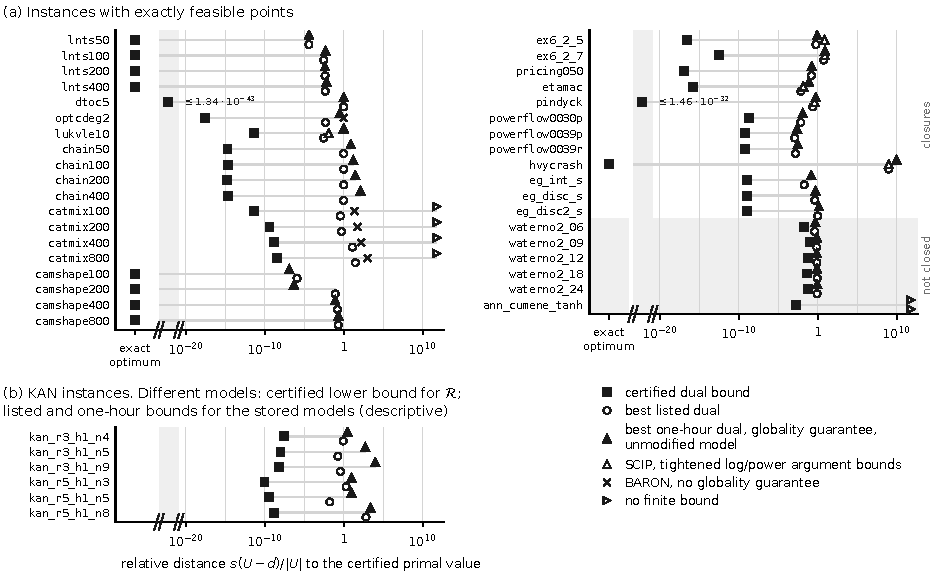
\includegraphics[width=\textwidth]{fig-headline}
\caption{Relative distance $\sense(\Uprim-d)/|\Uprim|$ of dual bounds $d$ from the certified primal value $\Uprim$ ($\sense=-1$ only for \inst{pricing050}).
(a)~Certified and listed dual bounds refer to the stored model.
The one-hour values are solver output on the GAMS files, and comparing them with the certified bounds assumes that the GAMS and OSIL forms agree where \cref{tab:sem-gams} checks this only at sample points; only filled triangles are bounds with a globality guarantee for the unmodified model.
Distances below $10^{-20}$ are drawn left of the second axis break, with their relative gaps.
(b)~$\Uprim$ is the objective at a point of $\RP$, and the square is a lower bound on $\vstar(\Rnet)\le\vstar(\RP)$; the other bounds concern the stored models.}
\label{fig:results-headline}
\end{figure}

% The two small tables may go only at the top or bottom of text pages: after
% the full-page tab:closures they are deferred and would otherwise fill a
% half-empty float page. The setting is local to this group.
% All floats of this section are input here, at its start, so that they print
% before Section 4 begins.
\begingroup\makeatletter\def\fps@table{!tb}\makeatother
% Generated by paper-open-minlplib/data/make_tables.py from data/numbers.json.
% Do not edit by hand; rerun the script. Requires booktabs, array and rotating;
% \inst{} typesets an instance name; underscores are not escaped (macros.tex).
\begin{table}
\centering
\footnotesize
\setlength{\tabcolsep}{4pt}
\caption{Improved bounds for the five \inst{waterno2} instances and \inst{ann_cumene_tanh} (not closed).
$L$: certified dual bound, rounded down. $U$: objective of an exactly feasible point, rounded up.
$\delta=(U-L)/\min(|L|,|U|)$, rounded up. Factor: $L$ divided by the best listed dual bound, rounded down.
\textsuperscript{a}The primal point is MINLPLib's listed point p4 made exactly feasible. The dual bound improved in three steps: 263.735099 (period Lagrangian, $\delta\le7.27\%$), 272.584700 (one slope vector per separator, with pair bounds over 113--162 cells per separator, $\delta\le3.78\%$), 278.230573 (cellwise slopes, $\delta\le1.68\%$).
\textsuperscript{b}$L^*=-7447080719734483\cdot2^{-41}$; MINLPLib lists no dual bound; the bound also holds for the algebraically identical \inst{ann_cumene_exp}.}
\label{tab:unclosed}
\begin{tabular}{@{}lllllll@{}}
\toprule
instance & $n$ ($n_{\mathrm{int}}$)/$m$ & best listed dual (solver) & $L$ & $U$ & $\delta$ & factor \\
\midrule
\inst{waterno2_06}\textsuperscript{a} & 996 (54)/1234 & $165.1902989$ (SCIP) & $278.230573$ & $282.888038$ & 1.68\% & 1.68 \\
\inst{waterno2_09} & 1494 (81)/1852 & $273.8958303$ (SCIP) & $824.834692$ & $914.012$ & 10.82\% & 3.01 \\
\inst{waterno2_12} & 1992 (108)/2470 & $479.5051427$ (Gurobi) & $2089.754565$ & $2233.821346$ & 6.90\% & 4.35 \\
\inst{waterno2_18} & 2988 (162)/3706 & $770.7361733$ (SCIP) & $4790.820715$ & $5023.983$ & 4.87\% & 6.21 \\
\inst{waterno2_24} & 3984 (216)/4942 & $1095.126488$ (SCIP) & $6576.151388$ & $6963.795181$ & 5.90\% & 6.00 \\
\inst{ann_cumene_tanh}\textsuperscript{b} & 794/790 & none & $-3386.5403$ & $-3379.9823940$ & 0.195\% & --- \\
\bottomrule
\end{tabular}
\end{table}

% Generated by paper-open-minlplib/data/make_tables.py from data/numbers.json.
% Do not edit by hand; rerun the script. Requires booktabs, array and rotating;
% \inst{} typesets an instance name; underscores are not escaped (macros.tex).
\begin{table}
\centering
\footnotesize
\setlength{\tabcolsep}{4pt}
\caption{The six KAN instances of our set. The OSIL models have no exactly feasible point; $\RP$ is the OSIL model without the partition-of-unity rows.
$L$: certified lower bound on $\vstar(\Rnet)\le\vstar(\RP)$, the weaker of two bounding codes, rounded down.
$U$: upper end of the objective enclosure at a point of $\RP$, rounded up. $U-L$ is computed from the exact ends and rounded up.
Listed dual (Gurobi in all six cases) and listed primal: MINLPLib page values; the listed points are feasible only within a tolerance.
Published SCIP~9.0.1 values with zero gap (Karia et al.): \textsuperscript{a}$0.00108116412047821$, at least $0.00170$ below $L$; \textsuperscript{b}$-0.0130809958982354$, at least $0.00203$ below $L$.}
\label{tab:kan}
\begin{tabular}{@{}llllll@{}}
\toprule
instance & listed dual & listed primal & $L$ & $U$ & $U-L$ \\
\midrule
\inst{kan_r3_h1_n4}\textsuperscript{a} & $0.0003908$ & $0.00278124$ & $0.002781237152581$ & $0.002781237221442$ & $6.89\cdot10^{-11}$ \\
\inst{kan_r3_h1_n5}\textsuperscript{b} & $-0.01302849$ & $-0.01104268$ & $-0.01104267952179$ & $-0.01104267941448$ & $1.08\cdot10^{-10}$ \\
\inst{kan_r3_h1_n9} & $0.0081425$ & $0.01296366$ & $0.01296365996347$ & $0.01296366005304$ & $8.96\cdot10^{-11}$ \\
\inst{kan_r5_h1_n3} & $-789.740197$ & $-262.3058993$ & $-262.8642259093$ & $-262.8642258850$ & $2.42\cdot10^{-8}$ \\
\inst{kan_r5_h1_n5} & $0.26787523$ & $0.27265451$ & $0.2725832538548$ & $0.2725832539567$ & $1.02\cdot10^{-10}$ \\
\inst{kan_r5_h1_n8} & $-45.00462396$ & $0.36062128$ & $0.06932786051052$ & $0.06932786060620$ & $9.57\cdot10^{-11}$ \\
\bottomrule
\end{tabular}
\end{table}

\endgroup

\subsection{Selection}\label{sec:results-selection}

Of our 43 instances, 41 lie among the 155 nonconvex instances that pass our selection funnel: they are listed as open, meet a width rule (small heuristic upper bounds on treewidth), and have relative gaps above $10^{-4}$ or infinite (a missing bound or point counts as infinite) both in the instance list and between the best listed dual bound and the best listed point (\cref{app:literature-funnel} gives the rules, the funnel and its caveats).
We chose the 43 in two rounds by judged tractability, the first 11 before the rules were fixed, so the 29 closures among the 155 are not a solve rate.
The other two closures, \inst{camshape100} and \inst{lnts50}, fail only the last condition: their best listed dual bounds were already within \sci{1.22}{-6} and \sci{3.9}{-5}, relative, of the best listed points and of our proved optima; for them what is new is the exact optimal value, its proof and an exactly feasible point.
Three programs, written in at least two separate agent sessions, reproduce every funnel count from the saved pages and width estimates; no separate agent session reviewed the code that estimated the widths and applied the rules.

\subsection{The 31 closures}\label{sec:results-closed}

Of the closures in \cref{tab:closures} (\cref{def:sem-certificate}, under \reading{b}), nine are attained exact optima: \inst{lnts50}--\inst{lnts400} (\cref{thm:lnts-opt}), \inst{camshape100}--\inst{camshape800} (\cref{thm:camshape-opt}) and \inst{hvycrash} (\cref{prop:hvycrash-identity}).
Eleven more have $\gaprel\le\sci{3.00}{-13}$, and the largest relative gap, that of \inst{catmix800}, is at most \sci{3.09}{-9}, more than 300 times below the tolerance $10^{-6}$ of MINLPLib's solved mark.
Of the 31 closures, 28 are continuous; the three \inst{eg} instances are mixed-integer.
For the 14 closures at evidence level \evid{rerun} (\cref{tab:trust}), the per-leaf or per-stage certificate data are not stored, so a check reruns the search or the stage computation; for the three \inst{eg} instances the leaf partition is stored and its coverage is checked exactly.

The class column of \cref{tab:closures} names the certificate class: \emph{staged}, a split along the stages of the model (\cref{sec:split}); \emph{comparison}, a discrete Sturm comparison along a chain of rows; \emph{dense rows}, a Lagrangian over a few dense coupling rows; \emph{convexity}, SDP duality, hidden convexity or concavity on a polytope; \emph{identity}, rows that force the objective value; and \emph{reduced space}, branch and bound over a few inputs with enclosures that keep cancellation (\cref{sec:other}).

\Cref{fig:results-headline} shows how far the listed bounds were from closing these instances: for 12 of the 31 closures the best listed dual bound lies below $\Uprim$ by more than $|\Uprim|/2$.
Our one-hour runs improve on the best listed dual bound for only five of the 43 instances (\cref{sec:solvers-campaign}).

\subsection{The other 12 instances}\label{sec:results-other}

\Cref{sec:split-waterno2} proves the dual bounds of \cref{tab:unclosed} for the five \inst{waterno2} instances, which schedule the pumps of a water supply network, and describes the points.
For \inst{ann_cumene_tanh}, a cumene process model with 14 tanh neural networks \citep{schweidtmann2019-deterministic-global-optimization-with-artificial}, MINLPLib lists no dual bound, and none of our one-hour runs gave a finite one; \cref{thm:ann-bound} gives our bound.

The six KAN instances of our set minimize trained KANs \citep{liu2024-kan-kolmogorov-arnold-networks} in the formulation of \citet{karia2025-deterministic-global-optimization-over-trained}.
Their stored models have no exactly feasible point, so their optimal value is $+\infty$ (\cref{prop:kan-infeasible}), and \cref{thm:kan-enclosure} encloses the optimal values of two related models, $\RP$ and its network relaxation $\Rnet$ (\cref{tab:kan}).
No KAN instance is closed, and our bounds do not concern the tolerance-feasible points of the stored models.

\subsection{Prior status}\label{sec:results-prior}

The prior-status column of \cref{tab:closures} summarizes the literature search of \cref{app:literature}; to our knowledge, within that search, no rigorous certificate had been published for any of the 31 stored models.
Seven closures have prior status \emph{fp closure} or \emph{fp near-closure} (\cref{sec:semantics-cert}): a floating-point closure or near-closure was reported for the same model, or, for \inst{dtoc5}, for a copy under assumed variable bounds.
Gurobi solved \inst{lnts50} and SCIP~8.1 solved \inst{eg_int_s} within their tolerances \citep{go2026-parabolic-approximation-relaxation-for-minlp,go2026-publisher-correction-parabolic-approximation-relaxation}.
The parabolic relaxation of \citet{go2026-clash-of-minlp-relaxations-piecewise} gives printed gaps of at most 0.01\% for \inst{lnts100}--\inst{lnts400}.
Octeract solved \inst{camshape100} \citep{bestuzheva2025-global-optimization-of-mixed-integer}.
MINOTAUR solved \inst{QPLIB_8585}, a copy of \inst{dtoc5}, after assuming default bounds for almost all variables \citep{mittelmann2026-continuous-non-convex-qplib-benchmark}.

Nine closures have prior status \emph{listed solve} (a benchmark page lists a solver as solving the instance or a copy, without a value or log that we can check), \emph{related model} (a result for a twin, a rounded copy or a source model), \emph{value only} (a value recorded without proof) or \emph{unread source} (a source that we could not read may contain a result).
Earlier versions of Mittelmann's benchmark page list MINOTAUR~0.2.1 as solving \inst{QPLIB_8803}, a copy of \inst{optcdeg2}, without value or log.
They also list Octeract, without value or log, as solving \inst{QPLIB_2480}, a rounded copy of \inst{camshape200} whose optimum is higher by more than $2\cdot10^{-6}$ relative (\cref{prop:camshape-copies}).
MINOTAUR is listed as solving \inst{QPLIB_3177}, a rounded copy of \inst{camshape800}; its reported value is not attainable by an exactly feasible point of the copy (\cref{prop:qplib-copies}).
ANTIGONE closed \inst{powerflow0030r}, the rectangular twin of \inst{powerflow0030p}, in floating point \citep{vigerske2026-minlplib-a-library-of-mixed}.
\Citet{ghaddar2016-optimal-power-flow-as-a} solved MATPOWER's case39 in floating point with the transformer taps that \inst{powerflow0039p} and \inst{powerflow0039r} drop.
The CUTE source file of \inst{hvycrash} records the value $-0.21850$ without proof \citep{toint2013-cute-hvycrash-source-sif-files}.
\Citet{mcdonald1997-glopeq-a-new-computational-tool}, which we could not read, may contain $\varepsilon$-global results for \inst{ex6_2_5} and \inst{ex6_2_7}.

The other 15 closures have prior status \emph{none}: we found no prior global result consistent with our certificates.
For the stored \inst{waterno2} models we found no closure; three possibly relevant sources could not be read (\cref{app:literature-unread}), and we claim no priority for period decomposition.

% Plan: development/outline.md, section 5, "§4". Proofs of the validity
% results and of thm:lnts-opt (with lem:lnts-elim, prop:lnts-support):
% Appendix G-proofs-split. Full proofs, computations and verification
% records of the certificates: supplement files B1 (lnts, lukvle10),
% B2 (dtoc5, optcdeg2), B4 (chain, catmix) and B8 (waterno2). The certificate
% boxes live in those supplement sections (round-1 adjudication G2-09); here one
% sentence per theorem names arithmetic, implementations and evidence level.
% Replay tiers are only in Table 7 and the boxes (round-2 adjudication G2-02).
% Part (c) of prop:split-affine and the last statement of prop:split-cellwise,
% with their proofs, moved to the supplement (prop:split-forced,
% prop:split-cellwise-best in B10-split-extras.tex; round-2 G2-01).
\section{Split certificates along stage structure}\label{sec:split}

Fifteen of the 31 closures form the staged class of \cref{tab:closures}: \inst{lnts50}--\inst{lnts400}, \inst{dtoc5}, \inst{optcdeg2}, \inst{lukvle10}, \inst{chain50}--\inst{chain400} and \inst{catmix100}--\inst{catmix800}; the \inst{waterno2} bounds use the same idea.
We cut the model along its stages, add to each stage a function of the variables that it shares with the next stage, and subtract the same function from the next stage, so that these terms cancel at every feasible point; rigorous lower bounds on the stage minima then sum to a dual bound.
The \inst{catmix} certificates use a variant: they bound the value functions of the stage recursion from below, and their validity rests on concavity of the true value functions (\cref{lem:split-minorant}).
\Cref{app:splitproofs} proves the validity results of \cref{sec:split-framework}; \cref{tab:staged} summarizes the certificates, and \cref{app:splitproofs-lnts,app:families} give their full proofs, certificate boxes and verification records.

\subsection{Path model and validity}\label{sec:split-framework}

Let $N\ge1$.
Bag $t\in\{1,\dots,N\}$ (a block of variables, as in a tree decomposition) holds a vector $z_t\in\R^{d_t}$, a set $K_t\subseteq\R^{d_t}$ (the bounds and the rows that involve only bag~$t$) and a cost $F_t\colon\R^{d_t}\to\R\cup\{+\infty\}$.
Consecutive bags share a separator: $\pi^R_tz_t=\pi^L_{t+1}z_{t+1}\in\R^{k_t}$ for $1\le t<N$, where $\pi^R_t$ and $\pi^L_{t+1}$ select coordinates.
The path model is
\begin{equation}\label{eq:split-path}
  \text{(P)}\qquad
  \vstar=\inf\Bigl\{\sum_{t=1}^NF_t(z_t) : z_t\in K_t,\ F_t(z_t)<\infty\ (1\le t\le N),\ \pi^R_tz_t=\pi^L_{t+1}z_{t+1}\ (1\le t<N)\Bigr\},
\end{equation}
with $\vstar=+\infty$ if its feasible set $\feas[\mathrm P]$ is empty.
The costs $F_t$ take the value $+\infty$ where an expression of the model is undefined; this encodes the domain rule of \cref{def:sem-model}(iv).
For a transcribed control problem, bag~$t$ is the stage $(x_t,u_t,x_{t+1})$ with its dynamics rows, and its separator is $x_{t+1}$; a variable of every stage, such as the step $h$ of \inst{lnts}, lies in every separator.

A \emph{split} is a tuple $\varphi=(\varphi_1,\dots,\varphi_{N-1})$ of real functions $\varphi_t\colon\R^{k_t}\to\R$; we put $\varphi_0=\varphi_N=0$.
For sets $K'_t\subseteq\R^{d_t}$ define
\begin{equation}\label{eq:split-bound}
  F^\varphi_t(z)=F_t(z)+\varphi_t(\pi^R_tz)-\varphi_{t-1}(\pi^L_tz),
  \qquad
  B(\varphi;K')=\sum_{t=1}^N\inf_{z\in K'_t}F^\varphi_t(z),
\end{equation}
with $\inf\emptyset=+\infty$ and the convention that a sum with a term $+\infty$ equals $+\infty$; write $B(\varphi)=B(\varphi;K)$.
We call $F^\varphi_t$ the \emph{stage residual} of bag~$t$.
We also call bag~$t$ the $t$-th stage; its \emph{stage problem} is the minimization of $F^\varphi_t$ over $K'_t$, with value the \emph{stage infimum}.
We call $K'_t$ an \emph{enclosure} if $K'_t\supseteq\proj_t\feas[\mathrm P]$, the set of bag-$t$ components of feasible points.
The \emph{split form} is the set of functions allowed for the $\varphi_t$: affine, quadratic, cellwise affine, and so on.

\begin{lemma}[split bound]\label{lem:split-bound}
Let $\varphi$ be a split.
\begin{enumerate}
\item[(a)] If every $K'_t$ is an enclosure, then $B(\varphi;K')\le\vstar$.
\item[(b)] \emph{Infeasibility.} Let every $K'_t$ be an enclosure.
  If $B(\varphi;K')=+\infty$, or if every $F_t$ vanishes on $K_t\cap\operatorname{dom}F_t$ and $B(\varphi;K')>0$, then $\feas[\mathrm P]=\emptyset$.
\item[(c)] \emph{Case split.} If $\feas[\mathrm P]\subseteq Z_1\cup\dots\cup Z_m$ and $\beta_c\le\inf\{\sum_tF_t(z_t):z\in\feas[\mathrm P]\cap Z_c\}$ for each $c$, then $\min_c\beta_c\le\vstar$.
  For a box $Z_c$, $\beta_c$ may be a bound of form (a) for the model restricted to $Z_c$, with its own split and enclosures.
\item[(d)] \emph{Row form.} Let $\psi_1,\dots,\psi_r$ be real functions of $z=(z_1,\dots,z_N)$ that vanish on $\feas[\mathrm P]$, such as linear combinations of rows, and let $\mu\in\R^r$ and $Y\supseteq\feas[\mathrm P]$.
  Then $\inf_{z\in Y}\bigl[\sum_tF_t(z_t)+\sum_k\mu_k\psi_k(z)\bigr]\le\vstar$, and $\feas[\mathrm P]=\emptyset$ if this infimum is positive and every $F_t$ vanishes on $K_t\cap\operatorname{dom}F_t$.
  With the copy rows $\pi^R_tz_t-\pi^L_{t+1}z_{t+1}$ as the $\psi_k$ and $Y=K'_1\times\dots\times K'_N$, this bound is $B(\varphi;K')$ for an affine split (\cref{prop:split-affine}).
\end{enumerate}
\end{lemma}

Since $\sum_tF^\varphi_t(z_t)=\sum_tF_t(z_t)$ at every feasible point, a certificate of form (a) must establish a rigorous lower bound on every stage infimum and the validity of the enclosures.

For nonempty control sets $U_i$ and maps $g_i\colon Y_{i-1}\times U_i\to Y_i$ ($1\le i\le n$), consider the dynamics $y_i=g_i(y_{i-1},u_i)$ with $y_i\in Y_i$ and $u_i\in U_i$.
For a terminal cost $\Phi\colon Y_n\to\R$, let $V_n=\Phi$ and $V_{i-1}(y)=\inf_{u\in U_i}V_i(g_i(y,u))$, so that $\vstar=\inf_{Y_0}V_0$.

\begin{lemma}[value-function minorants]\label{lem:split-minorant}
\begin{enumerate}
\item[(a)] If $W_0\le V_0$ on $Y_0$, then $\inf_{Y_0}W_0\le\vstar$.
\item[(b)] \emph{Chord interpolation.} Let $Y_{i-1}=Y_i=\R^2_+$ and $g_i(y,u)=M_i(u)y$ with every $M_i(u)$ entrywise nonnegative, and let $V_{i-1}$ be real-valued, concave and positively homogeneous on $\R^2_+$.
  Let $W_i\le V_i$ on $\R^2_+$, let $r_0=(1,0),r_1,\dots,r_J=(0,1)$ be vectors in $\R^2_+$ with strictly increasing angles, and let $w_j\le\inf_{u\in U_i}W_i(M_i(u)r_j)$ for every $j$.
  Then the chord interpolant, $W_{i-1}(\sigma r_j+\sigma'r_{j+1})=\sigma w_j+\sigma'w_{j+1}$ for $\sigma,\sigma'\ge0$, satisfies $W_{i-1}\le V_{i-1}$ on $\R^2_+$.
\end{enumerate}
\end{lemma}

Part~(b) uses concavity of the true $V_{i-1}$, which lies above its chords between rays, not of the computed $W_i$, so \cref{lem:split-minorant} is not an instance of \cref{lem:split-bound}.

\begin{proposition}[affine splits]\label{prop:split-affine}
Let $\varphi_t(s)=\lambda_t^\top s+c_t$ with $\lambda_t\in\R^{k_t}$ and $c_t\in\R$, and put $\lambda_0=\lambda_N=0$.
\begin{enumerate}
\item[(a)] $B(\varphi)$ does not depend on $c$.
  It is the Lagrangian dual function, at $\lambda$, of the copy formulation, in which every bag has its own copy of each separator coordinate and the copy rows $\pi^R_tz_t-\pi^L_{t+1}z_{t+1}=0$ are dualized with multipliers $\lambda_t$.
\item[(b)] \emph{Exactness.} If some $\bar z\in\feas[\mathrm P]$ has $\bar z_t\in\argmin_{K_t}F^\varphi_t$ for every $t$, then $B(\varphi)=\vstar=\sum_tF_t(\bar z_t)$, and $\bar z$ is a global minimizer.
  Conversely, if $B(\varphi)=\vstar$ and $\vstar$ is attained at $z^*$, then $z^*_t\in\argmin_{K_t}F^\varphi_t$ for every $t$.
\end{enumerate}
\end{proposition}

The slopes of an exact affine split are determined by the model: at a minimizer whose bag components are interior points of the $K_t$ at which the costs $F_t$ are differentiable, they are the copy-row multipliers, and after the dynamics rows are eliminated they are the discrete costates (\cref{prop:split-forced}, explanatory).
The affine certificates below take their slopes from a local KKT point; validity never depends on this choice.
Part~(b) is a stagewise exactness test; for convex stage problems at a stationary point it is a discrete form of the sufficiency condition of \citet{mangasarian1966-sufficient-conditions-for-the-optimal}.

\begin{proposition}[windows]\label{prop:split-window}
Let $K'_t$ be enclosures, $1\le a\le b\le N$, and
\begin{multline*}
  \beta_{[a,b]}(\varphi;K')=\inf\Bigl\{\sum_{t=a}^bF_t(z_t)+\varphi_b(\pi^R_bz_b)-\varphi_{a-1}(\pi^L_az_a) :\\
  z_t\in K'_t\ (a\le t\le b),\ \pi^R_tz_t=\pi^L_{t+1}z_{t+1}\ (a\le t<b)\Bigr\}.
\end{multline*}
Then $B(\varphi;K')\le\sum_{t\notin[a,b]}\inf_{K'_t}F^\varphi_t+\beta_{[a,b]}(\varphi;K')\le\vstar$.
Disjoint windows combine likewise.
\end{proposition}

A window loses nothing on its interior separators, at the price of one global problem in its free variables.

\begin{proposition}[cellwise slopes]\label{prop:split-cellwise}
For each separator $t\in\{1,\dots,N-1\}$ let $\mathcal P_t$ be a finite family of sets (cells) whose union contains $\pi^R_tz_t$ for every $z\in\feas[\mathrm P]$, and give each cell $D\in\mathcal P_t$ a slope $\lambda_{t,D}\in\R^{k_t}$.
Put $\mathcal P_0=\mathcal P_N=\{\ast\}$ with zero slope, and read the conditions $\pi^L_1z\in\ast$ and $\pi^R_Nz\in\ast$ as void.
Let $K'_t$ be enclosures, and for every $t$ and $(D,D')\in\mathcal P_{t-1}\times\mathcal P_t$ let $b_t(D,D')\in\R\cup\{+\infty\}$ satisfy
\[
  b_t(D,D')\le\inf\bigl\{F_t(z)+\lambda_{t,D'}^\top\pi^R_tz-\lambda_{t-1,D}^\top\pi^L_tz :
  z\in K'_t,\ \pi^L_tz\in D,\ \pi^R_tz\in D'\bigr\}.
\]
Then
\[
  \vstar\ \ge\ \mathrm{SP}:=\min\Bigl\{\sum_{t=1}^Nb_t(D_{t-1},D_t) : D_t\in\mathcal P_t\ (1\le t<N),\ D_0=D_N=\ast\Bigr\},
\]
the shortest-path value in the layered graph with arc weights $b_t$.
\end{proposition}

The only coupling condition is that the two bags at a separator use the same slope for the same cell; constants per cell cancel along every path, so a certificate stores slopes only.
With exact pair bounds on a partition and finite $\mathrm{SP}$, $\mathrm{SP}$ is also the largest bound that cellwise-affine splits with these slopes give (\cref{prop:split-cellwise-best}, explanatory).

\begin{remark}[derived enclosures]\label{rem:split-enclosures}
Several certificates use derived enclosures of unbounded states: the \inst{optcdeg2} velocities (\cref{lem:optcdeg2-enclosure}), the \inst{chain} end values (\cref{lem:chain-window}), the \inst{lukvle10} stage minimizers (\cref{lem:lukvle10-coercive}) and the \inst{waterno2} tank levels (\cref{lem:waterno2-levels}).
\end{remark}

\Cref{lem:split-bound}(a) is Krotov's sufficient condition for discrete control systems \citep{krotov1967-sufficient-conditions-for-the-optimality} as a Bellman inequality, related to relaxed dynamic programming \citep{lincoln2006-relaxing-dynamic-programming}: the split functions are Krotov's verification functions, and a split with $B(\varphi)=\vstar$ is a discrete calibration in the sense of the calculus of variations.
\Cref{prop:split-affine} is Lagrangian decomposition of copy rows, as in generalized Benders decomposition \citep{geoffrion1972-generalized-benders-decomposition} and in Lagrangian bounds within spatial branch and bound \citep{karuppiah2008-a-lagrangean-based-branch-and,khajavirad2009-a-deterministic-lagrangian-based-global,cao2019-a-scalable-global-optimization-algorithm}; and \cref{prop:split-cellwise} is closest to multistage decomposition with state copies and Lagrangian cuts \citep{zhang2022-stochastic-dual-dynamic-programming-for,fullner2022-non-convex-nested-benders-decomposition}, in particular cuts that differ across a partition of the state range \citep{yang2025-globally-converging-algorithm-for-multistage}.

\subsection{Exact affine splits: \inst{lnts} and \inst{dtoc5}}\label{sec:split-affine}

For $N\in\{50,100,200,400\}$, \inst{lnts}$N$ is the trapezoidal transcription with $N$ steps of length $h$ of the particle-steering problem of COPS~2.0 \citep{dolan2001-benchmarking-optimization-software-with-cops}.
A thrust of magnitude 100 in a steerable direction $\theta$ accelerates a particle from rest at the origin to height~5 and velocity $(45,0)$ in minimum time $Nh$.
With angles $\theta_j$, positions $p_j=(p^x_j,p^y_j)$, velocities $v_j=(v^x_j,v^y_j)$ ($0\le j\le N$) and $e(\theta)=(\cos\theta,\sin\theta)$, the model minimizes $Nh$ subject to
\[
  v_{i+1}-v_i=50h\bigl(e(\theta_i)+e(\theta_{i+1})\bigr),\qquad p_{i+1}-p_i=\tfrac h2(v_i+v_{i+1})\qquad(0\le i<N),
\]
$h\ge0$, zero initial states, $p^y_N=5$, $v^x_N=45$, $v^y_N=0$ and $|\theta_j|\le\bar\theta:=1.5707963267949$, a decimal that exceeds $\pi/2$ by between \sci{3}{-15} and \sci{4}{-15}; all other states are free.
Let $w_0=w_N=\frac12$ and $w_j=1$ otherwise; $c_0=(2N-1)/4$, $c_j=N-j$ for $0<j<N$ and $c_N=\frac14$; $r_j=c_j/w_j-N/2$; and $\alpha(h)=9/(20h)$, $\beta(h)=1/(20h^2)$.
For $\nu\ge0$ define
\begin{equation}\label{eq:lnts-g}
  C(\nu)=\sum_{j=0}^N\frac{w_j}{\sqrt{1+\nu^2r_j^2}},\qquad
  D(\nu)=\nu\sum_{j=0}^N\frac{w_jr_j^2}{\sqrt{1+\nu^2r_j^2}},\qquad
  g(\nu)=D(\nu)-\frac{20}{81}C(\nu)^2.
\end{equation}

\begin{theorem}[\inst{lnts} exact optimum]\label{thm:lnts-opt}
Let $N\in\{50,100,200,400\}$.
The function $g$ has exactly one positive root $\nu^*$.
The optimal value of \inst{lnts}$N$ is $\vstar=Nh^*$ with $h^*=9/(20\,C(\nu^*))$.
It is attained by $\theta^*_j=\arctan(\nu^*r_j)$, $h=h^*$ and the states that the dynamics determine.
The optimal values satisfy
\[
\begin{array}{ll}
  N=50: & 0.5546687649386788\le\vstar\le0.5546687649386789,\\
  N=100: & 0.5545954011669111\le\vstar\le0.5545954011669112,\\
  N=200: & 0.5545770161030836\le\vstar\le0.5545770161030837,\\
  N=400: & 0.5545724137006871\le\vstar\le0.5545724137006872.
\end{array}
\]
\end{theorem}

\Cref{app:splitproofs-lnts} gives the proof.
Summing the dynamics rows reduces exact feasibility to $h>0$, the angle bounds and three identities in the controls (\cref{lem:lnts-elim}).
At a fixed step $h$ the objective is the constant $Nh$; dropping it, combining these identities with multipliers $(\mu,\nu)$ and applying the Cauchy--Schwarz inequality to each control gives a support bound; this is \cref{lem:split-bound}(d) in its infeasibility form (\cref{prop:lnts-support}).
At $\mu=-\nu^*N/2$ the controls $\theta^*_j$, which follow the discrete linear-tangent law $\tan\theta^*_j=\nu^*(N/2-j)$ for $0<j<N$, attain the support bound; this proves optimality, and rational brackets of $\nu^*$ of width below $10^{-90}$ give the enclosures.
In the certificate (\cref{app:lnts-proof}), two separately written integer-only codes enclose the optima in arithmetic \arith{E}, one of them to the displayed digits; its evidence level is \evid{hand}+\evid{stored}.

\inst{dtoc5} is a discrete-time control problem with $T=49{,}999$ steps and $h=1/50000$:
\[
  \min\ h\sum_{t=0}^{T-1}(u_t^2+y_t^2)\quad\text{s.t.}\quad y_{t+1}=y_t+4hy_t^2-hu_t\quad(0\le t<T),\qquad y_0=1,
\]
with all other variables free; the final state $y_T$ does not enter the objective.
The CUTEst problem DTOC5 has $h$ in place of $4h$ \citep{luksan2026-cutest-source-forms-for-dtoc5,coleman1993-the-global-convergence-of-a}; our results concern the MINLPLib model only.

\begin{proposition}[\inst{dtoc5} dual identity]\label{prop:dtoc5-identity}
Write $c_t(x)=y_{t+1}-y_t-4hy_t^2+hu_t$, the negative of OSIL row~$t$.
Let $\lambda\in\R^T$ satisfy $\lambda_{T-1}=0$ and $\lambda_t<\frac14$ for $1\le t\le T-1$, and put $A_t=h(1-4\lambda_t)$ and $\bar y_t(\lambda)=(\lambda_t-\lambda_{t-1})/(2A_t)$.
Then every exactly feasible point $x$ satisfies
\begin{equation}\label{eq:dtoc5-squares}
  f(x)=q(\lambda)+h\sum_{t=0}^{T-1}\Bigl(u_t+\frac{\lambda_t}2\Bigr)^2+\sum_{t=1}^{T-1}A_t\bigl(y_t-\bar y_t(\lambda)\bigr)^2\ \ge\ q(\lambda),
\end{equation}
where $q(\lambda)=h(1-4\lambda_0)-\lambda_0-\frac h4\sum_{t=0}^{T-1}\lambda_t^2-\sum_{t=1}^{T-1}(\lambda_{t-1}-\lambda_t)^2/(4A_t)$.
\end{proposition}

\begin{proof}
At a feasible point $f(x)=f(x)+\sum_t\lambda_tc_t(x)$; collect the terms by variable.
The control $u_t$ contributes $hu_t^2+h\lambda_tu_t=h(u_t+\lambda_t/2)^2-h\lambda_t^2/4$.
The state $y_t$ with $1\le t\le T-1$ contributes $A_ty_t^2+(\lambda_{t-1}-\lambda_t)y_t=A_t(y_t-\bar y_t)^2-(\lambda_{t-1}-\lambda_t)^2/(4A_t)$, where $A_t>0$.
The fixed state $y_0=1$ contributes $h-\lambda_0-4h\lambda_0$, and $y_T$ contributes $\lambda_{T-1}y_T=0$.
\end{proof}

The identity needs no state enclosure or variable bound. It is an affine split with the dynamics rows kept in the bags and slopes $-\lambda_t$ on the separators $y_{t+1}$; $\lambda_{T-1}=0$ is necessary because the free $y_T$ would otherwise make the Lagrangian unbounded below.

\begin{theorem}[\inst{dtoc5} bracket]\label{thm:dtoc5-bracket}
Let $\hat x=(\hat u,\hat y)$ be the stored exactly feasible rational point (\cref{sec:points}), and set $\hat\lambda_t=-2\hat u_t$ for $t\le T-2$ and $\hat\lambda_{T-1}=0$.
Then $\hat\lambda_t<0$ for $t\le T-2$, and
\begin{align*}
  \vstar&\ge q(\hat\lambda)\ge5.38967211918114046742396649913627186883131268,\\
  \vstar&\le f(\hat x)\le5.38967211918114046742396649913627186883131341,
\end{align*}
with $f(\hat x)-q(\hat\lambda)\le\sci{7.21}{-43}$.
\end{theorem}

\begin{proof}
All rows hold at $\hat x$ in rational arithmetic, and $\hat u_t>0$ for $t\le T-2$, so $\hat\lambda_t<0<\frac14$ and \cref{prop:dtoc5-identity} applies; the certificate evaluates $q(\hat\lambda)$ and $f(\hat x)$.
\end{proof}

In the certificate (\cref{app:dtoc5-proof}), two separately written exact codes \arith{E} both give the displays; its evidence level is \evid{hand}+\evid{stored}.
The lower end in \cref{thm:dtoc5-bracket} is a rigorous rational evaluation below the dual function at $\hat\lambda$; we claim neither an exact dual value nor a zero duality gap.
The optimal value is attained (\cref{cor:dtoc5-attained}), and the Lagrangian dual and the order-one semidefinite relaxation are tight to within \sci{7.21}{-43} (\cref{rem:dtoc5-sdp}).

\subsection{Richer split forms}\label{sec:split-richer}

\inst{optcdeg2} controls a forced oscillator with a quadratic velocity term over $N=50{,}000$ Euler steps of length $h=1/2500$.
With $a=0.02h$ and $b=0.2h$ the model is
\[
  \min\ \frac h2\sum_{t=0}^Ny_t^2\quad\text{s.t.}\quad y_{t+1}=y_t+hv_t,\quad v_{t+1}=v_t+hu_t-ay_t-bv_t^2\quad(0\le t<N),
\]
with $|u_t|\le\frac15$, $v_t\ge-1$ for $0<t<N$, $y_0=10$, $v_0=v_N=0$ and $y_1,\dots,y_N$ free; the CUTEst problem OPTCDEG2 has $b/4$ in place of $b$ \citep{luksan2026-cutest-source-forms-for-dtoc5}.
At our exactly feasible point the control is $+\frac15$ for $3092\le t<47290$, $-\frac15$ before and after, and fractional at the two switching stages.
With the discrete costates $(p^y_t,p^v_t)$ as slopes, the stage residual of the affine split contains $-b\,p^v_{t+1}v_t^2$, which is concave in $v_t$ where $p^v>0$, that is, on both $u=-\frac15$ arcs.
On these arcs our point does not minimize the stage residual, so this affine split is not exact; a floating-point evaluation with refined costates puts its bound about 0.6258 below the optimal value.
The certificate therefore adds curvature in the velocity only: its split function on the state $(y_t,v_t)$ is $\varphi_{t-1}(y,v)=p^y_t\,y+p^v_t\,v+\frac{q_t}{2}(v-\bar v_t)^2$, where $\bar v$ is the velocity of a refined local solution.
The curvature $q_t$ makes the stage residual slightly convex in $v$ at the refined trajectory $\bar v$ on the $u=-\frac15$ arcs (\cref{fig:optcdeg2-calibration}); validity does not depend on these choices.

\begin{theorem}[\inst{optcdeg2} bound]\label{thm:optcdeg2-bound}
Let the split functions $\varphi_t$ be given by the stored binary64 split data $p^y,p^v,q,\bar v$, read as exact rationals.
Every exactly feasible point of \inst{optcdeg2} has objective at least $B$, the rigorous rational evaluation of the bound of \cref{lem:optcdeg2-krotov}, and $B\ge293.87607509587509237$.
An exactly feasible point has objective at most $293.87607509587509328$, so $\gapabs\le\sci{8.98}{-16}$ and $\gaprel\le\sci{3.06}{-18}$.
\end{theorem}

\Cref{app:optcdeg2-proof} proves it with \cref{lem:split-bound}(a) and velocity enclosures $V_t\subseteq[-1,1.2135]$ from one forward and one backward pass through the dynamics with outward rounding.
In each stage residual, $y$ enters as a quadratic with positive leading coefficient and is eliminated in closed form, and $u$ enters through one affine expression; the remaining polynomials in $v$, of degree at most four, are bounded below with exact Sturm sequences, and the stage bounds, rounded down to the grid $2^{-200}$, are summed as integers.
In the certificate (\cref{app:optcdeg2-proof}), one exact code \arith{E} gives the displayed bound, and a separately written binary64 interval code certifies the weaker bound 293.8760750958728; its evidence level is \evid{stored}.

\inst{chain}$N$ is the trapezoidal transcription, with $N$ intervals, of the hanging chain of COPS~2.0 \citep{dolan2001-benchmarking-optimization-software-with-cops}: a chain of length~4 hangs between $(0,1)$ and $(1,3)$ with minimal potential energy (\cref{app:chain-model}).
The variables are the heights $x_i$ and slopes $u_i$ ($0\le i\le N$); the dynamics and the length row are equalities, and only the end heights are fixed.

\begin{theorem}[\inst{chain} bounds]\label{thm:chain-bound}
For $N\in\{50,100,200,400\}$, the optimal value of \inst{chain}$N$ is at least a binary64 number $L_N$, displayed rounded down in \cref{tab:closures}.
Exactly feasible points with coordinates in a real quadratic field give $\gapabs\le\sci{9.58}{-15}$, \sci{1.01}{-14}, \sci{9.34}{-15} and \sci{9.78}{-15}, respectively.
\end{theorem}

\Cref{app:chain} gives the proof.
The linear rows express the variables $x_i$ and $u_i$ through the vertex heights $z_1,\dots,z_N$ of a polyline over a fixed horizontal mesh; its two end pieces depend only on the end values $z_1$ and $z_N$ (\cref{lem:chain-polyline}).
Summation by parts then writes the objective with the cumulative length $v$ of the polyline as a second state, started at a free value $V$.
For a parameter $H>0$ let $G_H(v)=\frac12\bigl(v\sqrt{H^2+v^2}+H^2\operatorname{asinh}(v/H)\bigr)$ and $c_H=2G_H(1/(2N))$.
For the split $\varphi_k(z,v)=G_H(v)-vz-k\,c_H$, a closed-form inequality makes every interior stage residual nonnegative, with equality exactly on discrete catenaries (\cref{lem:chain-calibration}).
So the objective is at least an explicit function $B_N(z_1,z_N;V,H)$ of the end values, for all $V$ and all $H>0$ (\cref{prop:chain-endvalue}).
In this split the multiplier of each height difference is the cumulative length, which varies with the configuration as the tension of a real chain does; a fixed multiplier on the length row, a reverse-convex equality, gives only about 4.77 against an optimum of about 5.07 (floating-point grid estimate).
A two-dimensional interval branch and bound over the bounded region of \cref{lem:chain-window} then proves, on each leaf box, either $B_N\ge L_N$ for some $(V,H)$ chosen for that box, or that the box contains no feasible end values (\cref{lem:split-bound}(c), with (a) in each box).
In the certificate (\cref{app:chain-bnb}), two separately written interval codes \arith{I} certify the same four values; its evidence level is \evid{rerun}, because the search trees are not stored.

\inst{catmix}$N$ transcribes the catalyst mixing problem of COPS~2.0 \citep{dolan2001-benchmarking-optimization-software-with-cops}.
Its rows are $P(u_{i+1})x_{i+1}=Q(u_i)x_i$ ($0\le i<N$), with controls $u_i\in[0,1]$, states $x_i\in\R^2$, $x_0=(1,0)$, and $2\times2$ matrices that are affine in the control and contain a coefficient $c$ (\cref{app:catmix-model}).
The objective $x_{1,N}+x_{2,N}-1$ is minus the yield, about $-0.048$.
The GAMS file has $c=9a$ with $a=1/(2N)$; the OSIL file stores $c$ as a binary64 product that exceeds $9a$ by at most $5\cdot10^{-18}$.

\begin{theorem}[\inst{catmix} bounds]\label{thm:catmix-bound}
For $N\in\{100,200,400,800\}$, the optimal value of \inst{catmix}$N$ is at least a binary64 number $L_N$, displayed rounded down in \cref{tab:closures}; this also holds for the model with $c=9a$.
Exactly feasible points give $\gapabs\le\sci{1.85}{-13}$, \sci{1.90}{-11}, \sci{6.81}{-11} and \sci{1.49}{-10}, respectively.
\end{theorem}

\Cref{app:chain} also gives this proof: for fixed controls the rows determine the states, and the stage maps $M(u)=Q(u)P(u)^{-1}$ are entrywise nonnegative, so the objective plus one is $\mathbf 1^\top P(u_N)^{-1}M(u_{N-1})\cdots M(u_1)Q(u_0)x_0$, with each control in one factor.
The value functions of this dynamic program are concave, positively homogeneous and nonnegative on $\R^2_+$, and the certificate computes chord minorants of them backward over the stages on grids of several thousand rays (\cref{lem:split-minorant}(b)).
At fixed controls the objective does not increase when $c$ increases, which transports the bounds to $c=9a$.
In the certificate (\cref{app:catmix-computation}), one code gives the displayed bounds in arithmetic \arith{F} with $+,-,\times,\div$ only, and a separately written code certifies bounds at most \sci{3.7}{-10} lower.
The bounds have evidence level \evid{rerun}, since the per-stage chord values are not stored; the points have level \evid{stored} (exact rational state evaluation).

\subsection{Affine split plus window: \inst{lukvle10}}\label{sec:split-window}

\inst{lukvle10} is problem 5.10 of Luk\v{s}an and Vl\v{c}ek with $n=1000$, in the form distributed with CUTEst \citep{gould2015-cutest-a-constrained-and-unconstrained,luksan2026-cutest-source-forms-for-dtoc5}.
Its 1000 variables are free, and with $F(a,b)=(a^2)^{b^2+1}+(b^2)^{a^2+1}$ it reads
\[
  \min\ \sum_{i=0}^{499}F(x_{2i},x_{2i+1})\quad\text{s.t.}\quad 1-x_j+3x_{j+1}-2x_{j+2}-2x_{j+1}^2=0\quad(0\le j\le997).
\]
Row $j$ defines $x_{j+2}$ from $(x_j,x_{j+1})$, so the feasible points are indexed by $(x_0,x_1)$.

\begin{theorem}[\inst{lukvle10} bracket]\label{thm:lukvle10-bracket}
The optimal value of \inst{lukvle10} satisfies
\[
  352.2380254050784\le\vstar\le352.2380254064957;
\]
hence $\gapabs\le\sci{1.42}{-9}$ and $\gaprel\le\sci{4.03}{-12}$.
\end{theorem}

\Cref{app:lukvle10-proof} gives the proof.
Dualizing rows 0 to 993 and keeping rows 994 to 997 (\cref{lem:split-bound}(d), with $Y$ the set where the kept rows hold) separates the Lagrangian into 497 two-variable pair problems and a window over the last three pairs, the row-form analogue of \cref{prop:split-window}.
The window covers the end of the chain, where the best known point leaves the saddle fixed point $-1/\sqrt2$ of the recurrence and the pair Lagrangians are nonconvex.
The dualized rows give each squared variable a coefficient $q\in[-0.8156,0]$, so each pair Lagrangian grows at least like $(1+q)t^2$ in each variable~$t$, and each infimum over $\R^2$ is a minimum over an explicit box (\cref{lem:lukvle10-coercive}).
Least-squares KKT multipliers at MINLPLib's point p5, with one common value on the middle of the chain, leave 35 distinct problems for interval branch and bound.
The summed branch-and-bound tolerances dominate the certified gap; global optimality of the exactly feasible point is not proved.
In the certificate (\cref{app:lukvle10-proof}), one code gives the displayed bound and a separately written one certifies 352.238025369202; both use interval arithmetic \arith{I} with \texttt{mpmath}'s interval $\exp$ and $\log$, and the evidence level is \evid{rerun}.

\subsection{Large stages: \inst{waterno2}}\label{sec:split-waterno2}

The \inst{waterno2} instances schedule nine pumps in four stations of a network with one reservoir and three tanks \citep{huang2019-optimal-operation-of-water-supply} over $T\in\{6,9,12,18,24\}$ hourly periods, at minimal pumping cost.
Removing the $3(T-1)$ rows that copy the tank levels between periods and one horizon row leaves $T$ periods of 166 variables (9 binary) and 203 rows each; the separators are the three tank levels.
The horizon row requires the total inflow to be at least $r_T$, the exact sum of the demands, so it is equivalent to a terminal-volume row on the last period (\cref{lem:waterno2-horizon}).

For level slopes $\lambda_t\in\R^3$ and a horizon multiplier $\mu\ge0$, the period Lagrangian gives $\vstar\ge\mu r_T+\sum_tB_t$ for lower bounds $B_t$ on the Lagrangian of each period (\cref{prop:waterno2-lagrangian}).
This is \cref{lem:split-bound}(a) for an affine split, with the horizon row dualized as well, which is valid because $\mu(r_T-\sum_th_t)\le0$ at every feasible point ($h_t$ is the inflow of period~$t$).
It certifies \inst{waterno2_09}--\inst{waterno2_24}, with multipliers from a bundle method that was stopped early.
Because pump costs depend nonconvexly on the tank levels, an affine split can leave the stage minimizers of consecutive periods at different level vectors, which weakens the bound.
For \inst{waterno2_06} we therefore divide the range of the three tank levels at each separator into 148 to 240 cells, each with its own slope vector (\cref{prop:split-cellwise}); the bound rises from 263.735099 ($\gaprel\le7.27\%$) to 278.230573 ($\gaprel\le1.68\%$).
The arc weights $b_t$ follow, through an exact linear correction (\cref{lem:waterno2-reuse}), from 49,315 rigorous bounds for single periods over pairs of level boxes, and the exact shortest-path value is $39157472136693483/2^{47}$.
Each period or pair bound comes from a spatial branch and bound with polyhedral relaxations and safe LP bounds \citep{neumaier2004-safe-bounds-in-linear-and}, which discards every box whose bound reaches a preset target value.
SCIP and HiGHS supply only multipliers, targets and dual vectors, which affect the strength of the bounds but not their validity; this matters because SCIP~10 returned wrong optimal values on some period subproblems of \inst{waterno2_06} (\cref{sec:solvers-invalid}).

\begin{theorem}[\inst{waterno2} dual bounds]\label{thm:waterno2-bounds}
For $T=6,9,12,18,24$, the optimal value of \inst{waterno2_T} is at least 278.230573, 824.834692, 2089.754565, 4790.820715 and 6576.151388, respectively, and exactly feasible points give $\gaprel\le1.68\%$, $10.82\%$, $6.90\%$, $4.87\%$ and $5.90\%$.
\end{theorem}

The bounds are 1.68 to 6.21 times the best listed dual bounds (\cref{tab:unclosed}); no instance is closed.
Regenerating the SCIP-derived targets gives slightly lower, also valid bounds for \inst{waterno2_18} and \inst{waterno2_24} (\cref{app:repro-regen}).
The point for \inst{waterno2_06} is MINLPLib's listed point p4 made exactly feasible (\cref{sec:points}); the other four are ours.
All five points use identities of the decimal data such as $0.7^3=0.343$; this identity matters for the SCIP error of \cref{sec:solvers-invalid}.
In the certificate (\cref{app:waterno2-verification}), either of two separately written branch-and-bound codes yields every value, one with node bounds in \arith{F} and one in \arith{E}; corrections, sums and the shortest path are exact \arith{E}.
Its evidence level is \evid{rerun}, because the search trees are not stored.

% Plan: development/outline.md, section 5, "§5". Full proofs and data are in
% the supplement (app:camshape, app:small, app:powerflow, app:eg,
% app:egrounding, app:annkan); this section keeps statements, proof ideas,
% one certificate sentence per result and the essential numbers. The
% certificate boxes are in the supplement (round-1 item G3-02). Material moved
% to the supplement: development/moves/m-other.md. Replay times: section 10.
\section{Other certificate classes}\label{sec:other}

The other 16 closures of \cref{tab:closures} fall into the five certificate classes of \cref{sec:results-closed}, one per subsection: \emph{comparison} (\inst{camshape}), \emph{dense rows} (\inst{ex6_2_5}, \inst{ex6_2_7}, \inst{pricing050}), \emph{convexity} (the three \inst{powerflow} instances, \inst{etamac}, \inst{pindyck}), \emph{identity} (\inst{hvycrash}) and \emph{reduced space} (the three \inst{eg} instances), whose method also bounds \inst{ann_cumene_tanh} and the KAN relaxations (\cref{tab:unclosed,tab:kan}).
\Cref{app:camshape,app:small,app:powerflow,app:eg,app:annkan} give the full proofs and the certificate boxes.

%---------------------------------------------------------------------------
\subsection{Comparison along a chain: \inst{camshape}}\label{sec:other-camshape}

The four \inst{camshape} instances are the COPS cam design problem \citep{dolan2001-benchmarking-optimization-software-with-cops} in scalar GAMS form: maximize the valve-opening area of a convex cam, written as a minimization.
For $n\in\{100,200,400,800\}$ there are radii $r_1,\dots,r_n$ at equally spaced angles and differences $d_1,\dots,d_{n-1}$; with the constant $r_0:=1$ (the base circle) the model reads
\begin{equation}\label{eq:camshape-problem}
\begin{aligned}
\min\ & -c_0\textstyle\sum_{j=1}^{n} r_j\\
\text{s.t.}\ & G_j:\ -r_{j-1}r_j+c\,r_{j-1}r_{j+1}-r_jr_{j+1}\le 0\ \ (1\le j\le n-1),\\
& G_n:\ c_2r_{n-1}-2r_n-r_{n-1}r_n\le 0,\qquad H:\ c_Hr_n^2-4r_n\le 0,\\
& D_i:\ r_i-r_{i+1}+d_i=0\ \ (1\le i\le n-1),\qquad |d_i|\le\alpha\ \ (i\ge2),\\
& 1\le r_1\le\bar u,\qquad 1\le r_j\le 2\ \ (2\le j\le n-1),\qquad \ell\le r_n\le 2 .
\end{aligned}
\end{equation}
The constants are 15-digit decimals of $c_0=\pi/n$, $c=2\cos\Delta\theta$, $c_2=4\cos\Delta\theta$, $\bar u=1/(2\cos\Delta\theta-1)$, $\ell=2-1.5\Delta\theta$ and $\alpha=1.5\Delta\theta$, where $\Delta\theta=2\pi/(5(n+1))$; in the files $c_H=c$, and $d_1$ is free because the GAMS model omits the COPS curvature row on the first pair.

Dividing $G_j$ by $r_{j-1}r_jr_{j+1}>0$ makes the rows $G_1,\dots,G_{n-1}$ linear in $u_j=1/r_j$ (with $u_0=1$):
$e_j(u):=u_{j-1}-c\,u_j+u_{j+1}\ge0$, the discrete form of $u''+u\ge0$, which is convexity of a curve in polar coordinates.
In exact rational arithmetic define the Chebyshev values $U_0=1$, $U_1=c$, $U_{m+1}=cU_m-U_{m-1}$; the comparison sequence $S_0=1$, $S_1=1/\bar u$, $S_{j+1}=cS_j-S_{j-1}$, and $R_j=1/S_j$ ($R_j=+\infty$ if $S_j\le0$); the bounds $B_1=\bar u$ and $B_j=\min(R_j,2)$ for $j\ge2$; the min-plus envelope $E_1=\bar u$ and $E_j=\min_{2\le k\le n}(B_k+\alpha|j-k|)$ for $j\ge2$; $d^E_i=E_{i+1}-E_i$; and $v_n=-c_0\sum_jE_j$.
The certificate consists of six finite checks:
(K1) $U_m\ge0$ for $m\le n-1$, a discrete disconjugacy condition \citep{bohner1996-linear-hamiltonian-difference-systems-disconjugacy};
(K2) $0<S_j\le1$ for $1\le j\le n$;
(K3) $E_{n-1}=E_n=2$;
(K4) $\bar u\le1+\alpha$;
(K5) $c_0>0$, $1\le\bar u\le2$, $0<c<2$, $c_2\le4$ and $0<\ell\le2$;
(K6) $c_H\le2$.

\begin{lemma}[discrete Sturm comparison]\label{lem:camshape-sturm}
Let $1\le N\le n$ and $u_0=1$. Then for $1\le j\le N$,
$u_j-S_j=U_{j-1}(u_1-S_1)+\sum_{k=1}^{j-1}U_{j-1-k}\,e_k(u)$.
Hence, if (K1) holds, $u_1\ge S_1$ and $e_k(u)\ge0$ for $k<N$, then $u_j\ge S_j$ for $j\le N$.
\end{lemma}

\begin{lemma}[min-plus envelope]\label{lem:camshape-envelope}
(a) If $r\le B$ componentwise and $|r_{j+1}-r_j|\le\alpha$ for $2\le j\le n-1$, then $r\le E$.
(b) Under (K2) to (K6), $(E,d^E)$ satisfies every row and bound of \eqref{eq:camshape-problem}.
\end{lemma}

\Cref{lem:camshape-sturm} follows by induction from $z_{j+1}=cz_j-z_{j-1}+e_j(u)$ for $z=u-S$; \cref{lem:camshape-envelope}(a) is the triangle inequality along the slope rows, and (b) a row-by-row check that uses the inequality between arithmetic and harmonic means where $E$ leaves the comparison radii $R_j$ (\cref{app:camshape-proof}).

\begin{theorem}[\inst{camshape} exact optimum]\label{thm:camshape-opt}
Let $n\in\{100,200,400,800\}$ and read the constants of \inst{camshape<n>} as rationals. Then (K1) to (K6) hold, and:
(a) every exactly feasible $(r,d)$ satisfies $r\le E$, hence has objective at least $v_n$;
(b) $(E,d^E)$ is exactly feasible;
(c) $v_n=\vstar$; the optimal solution is unique and equal to $(E,d^E)$, and $E$ is the greatest feasible radius vector;
(d) $v_n$ is rational; its floor and ceiling at 14 decimals are $L$ and $U$ in \cref{tab:closures}.
\end{theorem}

\begin{proof}[Proof sketch]
(a) Feasibility gives $r>0$, hence $e_j(u)\ge0$ and $u_1\ge S_1$; \cref{lem:camshape-sturm} gives $r\le B$, and the rows $D_i$ and \cref{lem:camshape-envelope}(a) give $r\le E$.
(b) is \cref{lem:camshape-envelope}(b).
(c) A feasible point with objective $v_n$ has $r\le E$ and $\sum_jr_j=\sum_jE_j$, so $r=E$.
\end{proof}

In the certificate (\cref{app:camshape-proof}), (K1)--(K6), $v_n$ and every row at $(E,d^E)$ are evaluated in \arith{E} without branching, and three separately written codes with their own readers (two exact, one with directed rounding) agree on $v_n$ to all printed digits; its evidence level is \evid{hand}+\evid{stored}.
Against $v_n$, the best listed dual bounds leave relative gaps of $1.22\cdot10^{-6}$, 8.27\%, 16.31\% and 19.93\%; for \inst{camshape100} and \inst{camshape200}, which BARON closes at tolerance level in our runs (\cref{prop:baron-camshape}; earlier results in \cref{sec:results-prior}), the gain over solver output is in rigor.

\begin{proposition}[tolerance deficit]\label{prop:camshape-deficit}
For $0\le\varepsilon<1$ there is an explicit bound $D_n(\varepsilon)$ (\cref{app:camshape-deficit}), rational for rational $\varepsilon$, such that every point that violates each row and bound of \inst{camshape<n>} by at most $\varepsilon$ has objective at least $v_n-D_n(\varepsilon)$.
For the $\varepsilon\le10^{-8}$ of \cref{tab:camshape-deficit}, $D_n(\varepsilon)\le0.61\,n^2\varepsilon$; for example $D_{400}(3\cdot10^{-10})\le2.81\cdot10^{-5}$ and $D_{800}(3\cdot10^{-10})\le1.13\cdot10^{-4}$.
\end{proposition}

The proof applies the identity of \cref{lem:camshape-sturm} to a point with violations at most $\varepsilon$; the row violations enter with the weights $U_m$ (up to 605.9 for $n=800$), and the bounds and slopes are relaxed by $\varepsilon$.
$D_n$ is a proved upper bound, not the worst case; explicit $\varepsilon$-feasible points reach about 87\% of it (numerical evidence, \cref{fig:camshape-deficit}).
MINLPLib's points p2 of \inst{camshape400} and \inst{camshape800} violate rows by up to $3.0\cdot10^{-10}$ and lie at least $8.15\cdot10^{-6}$ and $3.27\cdot10^{-5}$ below $v_n$, about 29\% of $D_n(3\cdot10^{-10})$: they are feasible only within a tolerance (category~A).

%---------------------------------------------------------------------------
\subsection{Lagrangians over a few dense rows}\label{sec:other-dense}

Dualizing a few dense coupling rows leaves blocks of dimension two or one, each minimized rigorously: for the equality rows of \inst{ex6_2_5} and \inst{ex6_2_7} this is the row form of the split bound, \cref{lem:split-bound}(d), and for the inequality rows of \inst{pricing050} Lagrangian weak duality.

\paragraph{Gibbs free energy: \inst{ex6_2_5}, \inst{ex6_2_7}.}
Both minimize the Gibbs free energy $f(n)=\sum_pG_p(n_{\cdot p})$ of three components over three phases, with amounts $n_{ip}\in[10^{-7},b_i]$ and mass balances $\sum_pn_{ip}=b_i$; each $G_p$ is a UNIQUAC phase function (an ideal vapour for the third phase of \inst{ex6_2_5}) made of linear terms and terms $(\ell\cdot n_p)\ln(m\cdot n_p)$.
For $\lambda\in\R^3$ the balances give $f(n)=\lambda\cdot b+\sum_p[G_p(n_p)-\lambda\cdot n_p]$, with one phase per bracket.
Each $G_p$ satisfies $G_p(tn)=t\,G_p(n)+t\ln t\,\langle\rho_p,n\rangle$ for $t>0$, with $\rho_p$ the sum of the forms $\ell$; the source models have $\rho_p=0$, but the rounded constants of \inst{ex6_2_7} give $\rho_p=(0,0,5\cdot10^{-14})$.

\begin{theorem}[\inst{ex6_2_5}, \inst{ex6_2_7}]\label{thm:ex62-bounds}
For \inst{ex6_2_5}, $-70.7520778334477075803539469\le\vstar\le-70.7520778334477055803671220$, so $\gapabs\le2.00\cdot10^{-15}$.
For \inst{ex6_2_7}, $L\le\vstar\le U$ (\cref{tab:closures}), so $\gapabs\le4.82\cdot10^{-14}$.
The upper ends bound the objective at exactly feasible rational points.
\end{theorem}

\begin{proof}[Proof sketch]
Writing $n_p=ty$ with $t\in(0,T]$, $T=\sum_ib_i$, and $y$ in the simplex, the identity, $\rho_p\ge0$ and $t\ln t\ge-1/e$ give $G_p(n_p)-\lambda\cdot n_p\ge\min(0,Tm_p)-\max_i\rho_{p,i}/e$, where $m_p$ is a lower bound on the tangent-plane distance $G_p(y)-\lambda\cdot y$.
For $\lambda$ the 20-digit chemical potentials of a computed equilibrium, Gibbs' inequality bounds the vapour term, and two-dimensional interval branch and bound proves $m_p\ge-10^{-17}$ (\inst{ex6_2_5}) and $m_p\ge-6\cdot10^{-15}$ (\inst{ex6_2_7}) for the liquids (\cref{app:small-ex62}).
\end{proof}

\paragraph{Pricing: \inst{pricing050}.}
The only maximization instance has prices $x\in[0,10]^{50}$ and five demand rows:
$\max\,-c\cdot x$ subject to $\sum_ja_{ij}x_j\exp(g_{ij}x_j^{p_{ij}})\le r_i$, with integer $c_j\ge0$, $a_{ij}<0$, $g_{ij}<0$ and $p_{ij}\in\{1,2,3\}$.
Every term depends on one variable, so for every $\mu\in\R^5_{\ge0}$ and every feasible $x$,
\begin{equation}\label{eq:pricing-lagrangian}
-c\cdot x\ \le\ \mu\cdot r-\sum_{j=1}^{50}\min_{\xi\in[0,10]}\Bigl(c_j\xi+\sum_i\mu_ia_{ij}\,\xi\, e^{g_{ij}\xi^{p_{ij}}}\Bigr).
\end{equation}

\begin{theorem}[\inst{pricing050}]\label{thm:pricing-bound}
$-1813.8290784519730769\le\vstar\le-1813.8290784519730577$, where the upper end is a dual bound and the lower end the exact objective value of an exactly feasible point; $\gapabs\le1.92\cdot10^{-14}$.
\end{theorem}

\begin{proof}[Proof sketch]
Apply \eqref{eq:pricing-lagrangian} with two nonzero 20-digit multipliers; each one-dimensional minimum is certified on a partition of $[0,10]$ by proved signs of derivatives or an exact quadratic bound.
The primal point is a 17-digit KKT point with one coordinate raised by $1.27\cdot10^{-15}$; its row slacks are at least $3.4\cdot10^{-15}$ in interval arithmetic, and its objective is an exact rational (\cref{app:small-pricing}).
\end{proof}

The certificates bound boxes and univariate minima in \arith{I} and assemble the bounds in \arith{E}.
For \inst{ex6_2_5} and \inst{ex6_2_7} the displayed bounds come from one code, and a separately written code certifies slightly stronger ones; their evidence level is \evid{rerun}.
For \inst{pricing050} two codes reproduce the bound and two separately written codes check the point; its evidence level is \evid{stored}.

%---------------------------------------------------------------------------
\subsection{Global duality and convexity}\label{sec:other-convex}

\paragraph{AC optimal power flow.}
\inst{powerflow0030p}, \inst{powerflow0039p} and \inst{powerflow0039r} minimize generation cost on the MATPOWER networks case30 and case39 \citep{zimmerman2011-matpower-steady-state-operations-planning} under the AC power-flow equations, in polar (\texttt{p}) or rectangular (\texttt{r}) coordinates.
They drop two bus shunts of case30 and the transformer taps of case39 \citep{matpower2026-minlplib-power-flow-and-water}, so our bounds hold for the stored models only, not for MATPOWER's cases or the twin \inst{powerflow0030r}.
Rectangular voltages $e_k=v_k\cos\theta_k$, $f_k=v_k\sin\theta_k$ turn every flow row, for all real $v,\theta$, into $y_r=x^\top Q_rx$ with rational $Q_r$ and $x=(e_1,f_1,\dots,e_n,f_n)$, where $y$ collects flows and generator outputs.
Let $\mathcal Q$ be the set of $(x,y)$ that satisfy these identities, the balance and thermal rows, the boxes on $y$ and $\underline v_k^2\le e_k^2+f_k^2\le\bar v_k^2$; it omits the angle-difference and reference rows.
Every exactly feasible point maps into $\mathcal Q$ with the same cost, which depends on $y$ only.
Write the rows of $\mathcal Q$ as $\mathrm{lb}_r\le h_r=\sum_y(\ell_{r,y}y+q_{r,y}y^2)+x^\top Q_rx\le\mathrm{ub}_r$ and the cost as $c_0+\sum_y(c_{1,y}y+c_{2,y}y^2)$.

\begin{proposition}[weak duality with an eigenvalue shift]\label{prop:pf-duality}
Let $\lambda_r\in\R$ (equality rows) and $\mu^\pm_r\ge0$ (finite sides of inequality rows), $w_r=\lambda_r$ or $\mu^+_r-\mu^-_r$, $c(w)=c_0-\sum_{\mathrm{eq}}\lambda_r\mathrm{lb}_r-\sum\mu^+_r\mathrm{ub}_r+\sum\mu^-_r\mathrm{lb}_r$, $\kappa_y=c_{1,y}+\sum_rw_r\ell_{r,y}$, $\sigma_y=c_{2,y}+\sum_rw_rq_{r,y}$ and $A(w)=\sum_rw_rQ_r$.
If $\sigma\ge0$, every unboxed $y$ has $\sigma_y>0$ or $\kappa_y=0$, and $A(w)+\varepsilon I\succeq0$ for a rational $\varepsilon\ge0$, then every point of $\mathcal Q$ has cost at least
\[
\beta(w,\varepsilon)=c(w)+\sum_{y\ \mathrm{boxed}}\min_{t\in[l_y,u_y]}(\sigma_yt^2+\kappa_yt)-\sum_{y\ \mathrm{unboxed},\,\sigma_y>0}\frac{\kappa_y^2}{4\sigma_y}-\varepsilon\sum_k\bar v_k^2 .
\]
\end{proposition}

\begin{proof}
Adding $\lambda_r(h_r-\mathrm{lb}_r)=0$, $\mu^+_r(h_r-\mathrm{ub}_r)\le0$ and $\mu^-_r(\mathrm{lb}_r-h_r)\le0$ to the cost gives at least $c(w)+\sum_y(\sigma_yy^2+\kappa_yy)+x^\top A(w)x$; minimize each $y$-term and use $x^\top A(w)x\ge-\varepsilon\|x\|^2\ge-\varepsilon\sum_k\bar v_k^2$.
\end{proof}

An SDP solver proposes the multipliers, which are converted to rationals exactly, and exact $LDL^\top$ elimination proves semidefiniteness, as in verified SDP bounds \citep{jansson2007-rigorous-error-bounds-for-the,oustry2022-certified-and-accurate-sdp-bounds} and rational semidefiniteness certificates \citep{peyrl2008-computing-sum-of-squares-decompositions}.

\begin{theorem}[\inst{powerflow0030p}]\label{thm:pf-0030p}
Every exactly feasible point has objective at least $\Lcert=576.8934122988004$.
With the exactly feasible point of \cref{sec:points}, whose objective is at most $\Uprim=576.8934134704$, this gives $\gaprel\le2.04\cdot10^{-9}$.
\end{theorem}

\begin{proof}[Proof sketch]
\Cref{prop:pf-duality} with $\varepsilon=0$ and the stored multipliers on the 332 rows and 16 boxes of $\mathcal Q$: the sign conditions hold exactly, the $60\times60$ matrix $A(w)$ has 60 positive pivots, and the exact value $576.89341229880046984\ldots$ is truncated.
\end{proof}

The same $\beta$ bounds the Shor relaxation, so it is tight to the same gap (\cref{cor:pf-shor}); for the 39-bus models the Shor-type bound leaves a relative gap of about $3\cdot10^{-5}$ (numerical evidence), which a cut at bus~30 removes.
This bus has no load and one generator, with output $(P_g,Q_g)$, and its only branch, to bus~2, is a pure series susceptance $b=55.2486187845304$ in the stored models.
With $W_{kk}=e_k^2+f_k^2$, the flow and balance rows at bus~30 and Lagrange's identity give $W_{2,2}=F(P_g,Q_g,W_{30,30}):=W_{30,30}-2Q_g/b+(P_g^2+Q_g^2)/(b^2W_{30,30})$ at every point of $\mathcal Q$ (\cref{lem:pf-leaf}).
$F$ is convex for $W_{30,30}>0$, so an affine $H$ with $H\ge F$ at the eight vertices of a box satisfies $H\ge F$ on the box (\cref{lem:pf-planes}).
We do not claim this cut, the concave envelope of a rank-one $2\times2$ relation on a box, as new \citep[compare][]{chen2016-a-spatial-branch-and-cut}.

\begin{theorem}[\inst{powerflow0039p}, \inst{powerflow0039r}]\label{thm:pf-0039}
Every exactly feasible point has objective at least $41869.05148485014$ (\inst{powerflow0039p}), respectively $41869.05148327243$ (\inst{powerflow0039r}); with the points of \cref{sec:points}, $\gaprel\le6.33\cdot10^{-10}$, respectively $6.70\cdot10^{-10}$.
\end{theorem}

\begin{proof}[Proof sketch]
The bounds put $(P_g,Q_g,W_{30,30})$ in $B_0=[0,\frac{52}{5}]\times[\frac75,4]\times[\frac{2209}{2500},\frac{2809}{2500}]$, which the stored leaf boxes $B_1,\dots,B_m$ ($m=6$ and $9$) cover exactly.
On leaf $i$, add to $\mathcal Q$ the box $B_i$ and four rows $W_{2,2}\le H$ with $H\ge F$ at the eight vertices of $B_i$ (checked exactly); by \cref{lem:pf-leaf,lem:pf-planes} every exactly feasible point lies in one of these leaf relaxations.
\Cref{prop:pf-duality} applies verbatim to them, with each leaf's stored multipliers and a rational shift $\varepsilon_i$; for \inst{powerflow0039p}, whose stored multipliers also weight the angle rows, the leaf relaxations keep these rows (\cref{app:powerflow-0039}).
Because the eigenvalues of $A(w)$ come in pairs (\cref{prop:pf-double}), rounding near-optimal multipliers can create a negative pair: the stored \inst{powerflow0039r} certificate absorbs one, about $-6.07\cdot10^{-10}$, with $\varepsilon=10^{-9}$.
The stored \inst{powerflow0039p} certificate uses $\varepsilon=10^{-8}$; setting its tiny angle-row multipliers to zero gives a certificate that needs no shift (\cref{rem:pf-anglefree}), so no trigonometric bound enters any of the three dual proofs.
All shifts cost at most $4.4\cdot10^{-7}$.
\end{proof}

In the certificate (\cref{app:powerflow-verification}), both implementations share one OSIL reader, whose rows a separately written reader reproduced exactly; the first implementation's replay and a separately written exact replay, both in \arith{E}, reproduce or exceed every bound; the evidence level is \evid{stored}.

\paragraph{Hidden convexity: \inst{etamac}.}
This energy-economy model (97 variables, 70 rows, nine periods) minimizes the convex function $-\sum_t\beta_t\ln C_t$, $\beta_t>0$.
All rows are linear except nine production rows, which set new output to $\Phi_t=(a_tK\!N_t^{-p_1}+b\,L\!N_t^{-p_2}E\!N_t^{-p_3})^{-q}$; for $t=1$ a constant replaces the $K\!N$ term, and the row adds the constant $3.4653339648$ to $\Phi_1$.
With the source's exponents, $(p_2+p_3)q=1$ and $\Phi_t$ is concave, so relaxing the equalities to ``$\le$'' gives a convex program, a classical case of hidden convexity \citep{xia2020-a-survey-of-hidden-convex}; with the stored exponents, $s:=(p_2+p_3)q=1+4.14\cdot10^{-16}$ and $\Phi_t$ is not concave.

\begin{theorem}[\inst{etamac}]\label{thm:etamac-bound}
$-15.29467564336809217\le\vstar\le-15.29467564336808959$, so $\gapabs\le2.58\cdot10^{-15}$.
\end{theorem}

\begin{proof}[Proof sketch]
The rows give a box $\mathcal B$ that contains every feasible point.
On $\mathcal B$, $\Phi_t$ has a concave nondecreasing majorant: replace the aggregate $L\!N^{p_2q}E\!N^{p_3q}$ of degree $s$ by $\kappa$ times an aggregate of degree one, with $\kappa\ge\max(1,W^{s-1})$ for an upper bound $W$ on that degree-one aggregate over $\mathcal B$ (\cref{lem:etamac-majorant}).
The relaxation is convex, so its Lagrangian at a computed KKT point gives a tangent-plane bound over $\mathcal B$, evaluated in interval arithmetic (\cref{prop:etamac-tangent}).
The primal point fixes the investments $I_1,\dots,I_8$ and the new inputs $L\!N_t$ and $E\!N_t$ at stored 17-digit values and defines every other variable by one row (\cref{prop:pts-triangular}).
\end{proof}

\paragraph{Concavity on a polytope: \inst{pindyck}.}
This OPEC pricing model has 16 periods and 116 variables.
Given prices $p\ge0$, all other variables follow recursively; the fringe supply solves $s-a-b\,e^{-Ks}=0$ with $b>0$, whose left side increases strictly in $s$.
So the problem is to minimize $-J(p)$, the negative discounted profit, over a set $P=\{p\ge0:d_t(p)\ge0\ \forall t\}$ that contains the prices of all exactly feasible points ($d_t$: OPEC sales); $P$ is not known to be convex.

\begin{theorem}[\inst{pindyck}]\label{thm:pindyck-bound}
There is a polytope $G\supseteq P$ with $\nabla^2J\preceq-\mu I$ on $G$, $\mu=10^{-3}$.
With a computed approximate stationary point $p^*$ and $g=\nabla J(p^*)$, every exactly feasible point has objective at least $-J(p^*)-\|g\|^2/(2\mu)$, and
\[
-1170.486285436088562087577425069306\ \le\ \vstar\ \le\ -1170.486285436088562087577425069288,
\]
the upper end from an exactly feasible point with prices $p^*$; $\gapabs\le1.70\cdot10^{-29}$.
\end{theorem}

\begin{proof}[Proof sketch]
Lower bounds on the supply, certified by linear programs with exact weak duality, give $G$.
Implicit differentiation writes $\nabla^2J(p)=\Psi(\theta(p))$ through 112 per-period quantities $\theta$; on each leaf of a partition of a certified box $\Theta\supseteq\theta(G)$, an affine model of $\Psi$ and an $LDL^\top$ matrix test prove $\Psi\preceq-\mu I$ (\cref{lem:pindyck-matrix}).
Since $G$ is convex, $J(p)\le J(p^*)+g\cdot(p-p^*)-\frac\mu2\|p-p^*\|^2\le J(p^*)+\|g\|^2/(2\mu)$ for $p\in P$; enclosures of $J(p^*)$ and $\|g\|^2$ give the numbers (\cref{app:small-pindyck}).
\end{proof}

\begin{corollary}[unique minimizer]\label{cor:pindyck-unique}
\inst{pindyck} has a unique minimizer; its prices lie within Euclidean distance $2\|g\|/\mu\le3.7\cdot10^{-13}$ of $p^*$ (\cref{app:small-pindyck}).
\end{corollary}

Both certificates have evidence level \evid{stored} (\cref{app:small-etamac,app:small-pindyck}).
For \inst{etamac} (40-digit \arith{I}), the displayed bound comes from one code, a separately written code certifies the weaker $-15.294675643368096$, and one code encloses the primal value.
For \inst{pindyck} (exact LP certificates, matrix tests in \arith{F} and \arith{I}), two separately written codes prove the concavity ($\Psi$ derived twice without computer algebra and checked numerically); the displayed bound comes from one code's enclosures, a slightly weaker one from the other's, and two codes check the primal point.

%---------------------------------------------------------------------------
\subsection{An identity: \inst{hvycrash}}\label{sec:other-hvycrash}

\inst{hvycrash} is the CUTE problem HVYCRASH at its original size $N=50$ \citep{bongartz1995-cute-constrained-and-unconstrained-testing,toint2013-cute-hvycrash-source-sif-files}.
It has angles $\theta_0,\dots,\theta_{50}\in[0,6.2831854]$, controls $c_k\in[0.08,0.417]$, free $r_k,s_k$ ($1\le k\le50$), $s_0=0$, and with $h=4.37\cdot10^{-3}$, $D(c)=0.486237c^2+0.0162079>0$ and $A(c)=c/(0.3c^2+0.01)$ the 150 rows
\begin{align*}
&\text{acc}_k:\ s_{k-1}-s_k+h\cos\theta_k/(D(c_k)\,r_k^2)=0,\qquad
\text{alg}_k:\ -1/r_k-\cos\theta_k/(D(c_k)\,r_k^3)=0,\\
&\text{dyn}_k:\ 0.1\,\theta_{k-1}-0.1\,\theta_k+h\,A(c_k)/r_k^2-h\cos\theta_k/(D(c_k)\,r_k^4)=0 .
\end{align*}
The objective is to minimize $s_{50}$.

\begin{proposition}[\inst{hvycrash}]\label{prop:hvycrash-identity}
(a) Every exactly feasible point has $s_{50}=-50h=-0.2185$.
(b) There is an exactly feasible point.
Hence $\vstar=-0.2185$, attained at every exactly feasible point.
\end{proposition}

\begin{proof}
(a) At a feasible point the rows are defined, so $r_k\ne0$ (\cref{def:sem-model}).
Multiplying $\text{alg}_k$ by $-r_k$ gives $\cos\theta_k/(D(c_k)r_k^2)=-1$; then $\text{acc}_k$ reads $s_k=s_{k-1}-h$.

(b) By the same identity, $\text{dyn}_k$ becomes $\theta_k-\theta_{k-1}=\kappa/(-\cos\theta_k)$ with $\kappa=10h(A(c_k)+1)D(c_k)$.
With $c_k=0.08$, $\kappa<6.52\cdot10^{-3}$; define backwards $\theta_{50}=3$, $\theta_{k-1}=\theta_k-\kappa/(-\cos\theta_k)$, $r_k=(-\cos\theta_k/D(0.08))^{1/2}$ and $s_k=-kh$, which satisfy every row exactly while all $\cos\theta_k<0$.
Since $-\cos\theta\ge-\cos2.6>0.85$ on $[2.6,3]\subset(\pi/2,\pi)$, downward induction gives $\theta_{k-1}\ge3-50\kappa/0.85>2.6$ for every $k$, so all $r_k$ are real and nonzero and every bound holds (\cref{app:small-hvycrash}).
\end{proof}

The proof is at evidence level \evid{hand} (\cref{app:small-hvycrash}).
Computer checks confirm it but are not part of it: two codes checked the first witness and a third code a second witness in 60-digit \arith{I}, and three codes, with two separately written readers, matched the stored rows.
The identity concerns \reading{b} ($50\,\fl(4.37\cdot10^{-3})$ differs from $0.2185$ by about $10^{-17}$).
Within the search of \cref{app:literature}, no source states the identity or gives a feasible point (prior status in \cref{sec:results-prior}).
Under a tolerance a stage can be dropped by letting $r_k\to\infty$: MINLPLib's points p1 and p2, with objective $-0.21413=-0.2185+h$, drop the last stage ($r_{50}$ of order $10^{7}$ and $10^{9}$), a category~A case in the upward direction (\cref{sec:semantics-categories}).

%---------------------------------------------------------------------------
\subsection{Reduced-space branch and bound with enclosures that keep cancellation}\label{sec:other-bb}

In the remaining models every variable is an explicit function of a few inputs: seven for the \inst{eg} instances (three or four of them integer), five for \inst{ann_cumene_tanh}, three or five for the KAN instances.
Enclosures that bound each term separately fail there, because of cancellation (\inst{eg}) or the depth of the networks (\inst{ann_cumene_tanh}, KAN).
The certificates therefore use enclosures that keep cancellation, and per-box linear programs whose values are recomputed by weak duality, so the LP solver is not trusted \citep{neumaier2004-safe-bounds-in-linear-and,ninin2015-a-reliable-affine-relaxation-method}.
The dual bounds of this class have evidence level \evid{rerun}; their certificate boxes are in \cref{app:egrounding-trust,app:annkan-ann-verif,app:annkan-kan-enclosure}.

\paragraph{Gaussian-kernel rows: the \inst{eg} instances.}
\inst{eg_int_s}, \inst{eg_disc_s} and \inst{eg_disc2_s} share 28 row functions of seven inputs, $g_k(x)=\sum_{m=1}^{97}a_{km}\exp\bigl(\sum_{i}\gamma_{ki}(s_ix_i-z_{mi})^2\bigr)$ (plus a linear term in two side rows), with a fixed scaling $s\in\{1,\frac1{10}\}^7$, $\gamma_{ki}<0$ fixed within a row and the same centres $z_m$ in all rows.
The objective variable occurs only in 24 rows $x_{\mathrm{obj}}\ge c_k+g_k(x)$, so the problem is to minimize $\Phi(x)=\max_{k\le24}(c_k+g_k(x))$ subject to two side rows, a two-sided row, bounds and integrality (16, 1{,}764 and 3{,}751 integer assignments).

On a box with centre $c$, the exponents of all terms of a row share the quadratic part $\sum_i\gamma_is_i^2d_i^2$ in $d=x-c$, so a second-order Taylor model of the row has signed moments of the 97 terms as coefficients, and only its remainder is bounded in absolute value (\cref{lem:eg-taylor}).
The resulting affine bounds enter a linear program over the 24 minimax rows and the relaxed side rows, whose multipliers weak duality turns into a bound on $\Phi$ (\cref{lem:eg-boxtests}); on sampled boxes, bounds that add up the term ranges had median gaps 3.2 to 151 times larger, the ratio growing as the boxes shrink (numerical evidence, \cref{app:eg-computation}).

\begin{theorem}[\inst{eg_int_s}, \inst{eg_disc_s}, \inst{eg_disc2_s}]\label{thm:eg-bounds}
Assume \cref{hyp:fp-ieee}, the correctness of the model reader, the enclosure code, the accuracy auditor (a program that checks each library exponential and power value that the enclosure code uses; \cref{app:egrounding-auditor}), the exact arithmetic and the coverage checker, and the faithful execution and retention of the recorded run (\cref{thm:eg-trust}).
Read the decimal data as exact rationals. Then $L\le\vstar\le U$ with $L$ and $U$ from \cref{tab:closures}; $\gapabs\le6.46\cdot10^{-9}$, $5.76\cdot10^{-9}$ and $5.64\cdot10^{-9}$, and $\gaprel\le1.00\cdot10^{-9}$.
The upper ends bound the objective at exactly feasible points.
\end{theorem}

\begin{proof}[Proof sketch]
A separately written program takes the leaves of the search trees only as a proposed partition, proves exactly that they cover the domain, and certifies every leaf against a target at least the displayed lower bound, with padded binary64 enclosures and the exact box tests of \cref{lem:eg-boxtests}.
The paddings cover all rounding errors under \cref{hyp:fp-ieee} if every exponential and integer power used has relative error at most $10^{-14}$ (\cref{lem:eg-padding}); a rerun under the accuracy auditor checked this for all 63{,}017{,}129{,}222 such values with an outward-rounded exponential and exact power tests, found no violation and certified every leaf again (\cref{app:egrounding-run}).
The 28 rows hold at the primal points with positive slack in exact dyadic-rational arithmetic.
\end{proof}

The first implementation, the search that proposed the leaves, also certifies on its own, in outward-rounded interval arithmetic without library functions, the bounds for \inst{eg_int_s} and \inst{eg_disc_s} and for the part of \inst{eg_disc2_s} with $x_7\in[24,27]$, the last under a side condition on its LP multipliers (\cref{tab:eg-matrix}).

\paragraph{A neural-network surrogate: \inst{ann_cumene_tanh}.}
This model optimizes a cumene process through 14 tanh networks \citep{schweidtmann2019-deterministic-global-optimization-with-artificial}, with 794 variables, 789 equality rows and the purity row $x_{772}\ge0.999$.
Five inputs $u=(x_{723},\dots,x_{727})$ in a box $\mathcal U$ determine 779 of the other variables through 529 linear rows and 250 rows $x_v=\tanh(x_s)$, and an elimination without division in the remaining product rows gives the objective as an explicit function $f(u)$ (\cref{lem:ann-reduction}).
So every exactly feasible point has $u\in\Omega$ and objective $f(u)$, where $\Omega\subset\mathcal U$ is cut out by the two-sided bounds of 722 determined variables and the purity row (1{,}445 one-sided inequalities).

\begin{theorem}[\inst{ann_cumene_tanh}]\label{thm:ann-bound}
$f(u)\ge L^*=-7447080719734483\cdot2^{-41}>-3386.5403$ for every $u\in\Omega$.
Hence $\vstar\ge L^*$ for \inst{ann_cumene_tanh} and for \inst{ann_cumene_exp}, which writes $\tanh$ through $\exp$.
An exactly feasible point has objective at most $-3379.9823940$, so $\gaprel\le0.195\%$.
\end{theorem}

\begin{proof}[Proof sketch]
A branch and bound partitions $\mathcal U$ into 1{,}852{,}333 regions; on each, affine forms with one noise symbol per input and per neuron enclose every variable, so the linearization errors of the 250 neurons can cancel downstream, and weak duality over the cube of noise symbols bounds $f$ (\cref{lem:ann-duality}).
Two codes bound every region of the same partition in outward-rounded binary64 arithmetic without library transcendentals; each alone proves $f\ge L^*$, given the covering (the second code copied one idiom of the first, so it is not separately written in the sense of \cref{sec:semantics-protocol}; \cref{app:annkan-ann-verif}).
The primal point fixes rational inputs and defines all other variables by one row each (\cref{prop:pts-triangular}).
\end{proof}

\Citet{schweidtmann2019-deterministic-global-optimization-with-artificial} report no convergence within $10^5$~s; their reduced-space problem has the same five inputs but one inequality, so it may be a relaxation of the MINLPLib model.

\paragraph{Kolmogorov--Arnold networks.}
The six KAN instances of our set (\cref{tab:kan}) minimize trained KAN surrogates of the Rosenbrock function in three or five dimensions (\texttt{r3} or \texttt{r5} in the name) \citep{liu2024-kan-kolmogorov-arnold-networks,karia2025-deterministic-global-optimization-over-trained}.
Each edge function contains a cubic B-spline; the encoding selects the knot interval of each edge argument by binaries and big-M rows, builds the basis by Cox--de Boor rows that are bilinear in binaries and arguments, and adds per edge three partition-of-unity rows $\sum_mB_{e,m,p}=1$, $p=1,2,3$.
For exact B-splines these rows are identities on admissible arguments; with the stored 16-digit coefficients they fail by $10^{-17}$ to $10^{-15}$.

\begin{proposition}[infeasibility]\label{prop:kan-infeasible}
No KAN instance of our set has an exactly feasible point.
\end{proposition}

\begin{proof}[Proof sketch]
Fix the edge $e^*$ of \cref{tab:kan-edges}.
For each admissible knot interval $I_k$ of its argument $z$, the recursion rows make the basis variables rational polynomials in $z$, and the partition rows require three residual polynomials to vanish.
Exact computation over $\Q$ (Sturm sequences, resultants or greatest common divisors) shows that they have no common zero in $I_k$; two separately written codes did this computation (\cref{app:annkan-kan-infeasible}).
\end{proof}

So every number is a valid but vacuous dual bound for the OSIL models, and we bound two relaxations instead.
$\RP$ is the OSIL model without the partition-of-unity rows.
The network relaxation $\Rnet$ has as points the pairs $(u,k)$ of an input $u$ in the box of the model and a knot choice $k$ that put every edge argument in its interval and every hidden value in its box; its objective is the network output $F(u,k)$.
Their optimal values $\vstar(\Rnet)$ and $\vstar(\RP)$ are infima as in \cref{def:sem-feasible}; every point of $\RP$ projects to a point of $\Rnet$ with the same objective value (\cref{lem:kan-projection}), so $\vstar(\Rnet)\le\vstar(\RP)$.

\begin{theorem}[KAN enclosure]\label{thm:kan-enclosure}
For each of the six instances, with $L$ and $U$ from \cref{tab:kan},
$L\le\vstar(\Rnet)\le\vstar(\RP)\le U$,
where $U$ is the upper end of an enclosure (width $\le3.2\cdot10^{-89}$) of the objective at a point of $\RP$.
$U-L\le2.42\cdot10^{-8}$ for \inst{kan_r5_h1_n3} and $\le1.08\cdot10^{-10}$ for the other five.
\end{theorem}

\begin{proof}[Proof sketch]
Two branch-and-bound codes over the input box bound $F$ for all admissible knot choices at once: path~(I) on the model's own polynomial pieces, path~(II) on the ideal $C^2$ spline network minus a perturbation term of at most $1.4\cdot10^{-10}$, bounded in exact arithmetic.
The reported $L$ is the weaker of the two bounds, so it is valid if either code is correct, given their shared OSIL reader, rigorous exponential and interval core; path~(II) assumes, without a check, that no NaN bound occurred.
A code review in a separate agent session found that the original path~(I) bound routine assumes exact halving of a binary64 curvature, which fails for some subnormal inputs; a replay with a guarded routine, proved valid for all finite inputs, reproduced all six searches and their bounds bit for bit, with no guard triggered (\cref{app:annkan-kan-enclosure}).
The points of $\RP$ fix binary64 inputs and knot choices and define the other variables row by row (\cref{prop:pts-triangular}); all OSIL bounds hold, and exact rational intervals enclose the objective.
\end{proof}

\Cref{thm:kan-enclosure} says nothing about points that satisfy the OSIL rows only within a tolerance, such as MINLPLib's listed points (partition rows violated by about $10^{-15}$); the zero-gap optima published for \inst{kan_r3_h1_n4} and \inst{kan_r3_h1_n5} lie below $L$ (\cref{sec:solvers-tolerance}).

% Plan: development/outline.md, section 5, "§6". Proposition prop:pts-exact and
% Remark rem:lukvle10-seeds are stated in the supplement (app:points).
% Final build of round 3 (sol-status 2): the pricing050 point is checked by two
% separately written codes (development/dossiers/small-checks/pricing_check.py and
% r2/pricing_check.py; the r2 session did not read the earlier check before writing
% its own), as in B5-small, C-points, tab:points-all and the register.
\section{Exactly feasible points}\label{sec:points}

The objective value at a point is a proved upper bound on $\vstar(\model)$ only if the point is proved to lie in $\feas$ \citep[Sect.~20]{neumaier2004-complete-search-in-continuous-global}.
A point computed in floating point satisfies nonlinear equality rows only up to rounding, so its objective value can even lie below a valid dual bound (\cref{lem:sem-enclosure}(b)), and rounding it to rationals almost never makes nonlinear equalities hold.
Every primal value $\Uprim$ in this paper is therefore the upper end (for \inst{pricing050}, the lower end) of a rigorous enclosure of the objective at a point that we prove satisfies every row, bound and integrality requirement of the stored model exactly; for the six KAN instances the point lies in $\RP$ (\cref{prop:kan-infeasible}).

\subsection{Four constructions}\label{sec:points-constructions}

Each construction starts from a numerical candidate; a proof then decides every row, bound and integrality requirement, exactly or over an outward-rounded enclosure within the bounds (\cref{tab:points-all} gives the construction of each point).
\begin{description}\setlength{\itemsep}{0pt}\setlength{\parsep}{0pt}
\item[Explicit exact points] have coordinates in $\Q$ or in a quadratic field $\Q(\sqrt D)$; signs in $\Q(\sqrt D)$ are decidable, and a \texttt{sqrt} node is accepted if the root is nonnegative and squares to the argument (\cref{prop:pts-exact}).
\item[Triangular definitions] fix seed values and define each further variable or block by rows in which it is the only unknown (\cref{prop:pts-triangular}).
\item[Interval existence proofs] use a Krawczyk test with fixed coordinates (\cref{thm:pts-krawczyk}), an intermediate-value bracket in one variable, or a scalar interval test for each implicit state.
\item[Strictly interior points] of models whose rows are all inequalities are proved by outward enclosures of the row bodies, with bounds and integrality checked exactly.
\end{description}
In triangular definitions and interval existence proofs, certificate data define the point: seeds and a recursion, a box and a square system, or a bracket and a sign change; for \inst{catmix} the recursion gives exact rationals.
We claim no stored decimal vector of these points, such as a box centre, to be exactly feasible.
The results below are proved in \cref{app:points}.

\begin{theorem}[Krawczyk test on a square subsystem with fixed coordinates]\label{thm:pts-krawczyk}
Fix $n-m$ coordinates of the variables of $\model$ at rational values $\xi$, and write the remaining $m$ coordinates as $z\in\R^m$.
Let $E$ be a set of $m$ rows of $\model$ and, for $i\in E$, let $t_i$ be a finite bound of row $i$ (its right-hand side if the row is an equality).
Let $G\colon\R^m\to\R^m$ have components $G_i(z)=g_i(\xi,z)-t_i$, where $g_i$ is the body of row $i$.
Let $X\subset\R^m$ be a closed box with finite, positive widths, and let $y\in X$.
Assume:
\begin{itemize}\setlength{\itemsep}{0pt}\setlength{\parsep}{0pt}
\item[(a)] every $G_i$ is defined and continuously differentiable on an open set containing $X$;
\item[(b)] $\mathbf{A}$ is an interval matrix with $G'(z)\in\mathbf{A}$ for all $z\in X$; $\mathbf{v}$ is an interval vector with $G(y)\in\mathbf{v}$; $C$ is a real $m\times m$ matrix; and $\mathbf{B}$ is an interval matrix with $I-CA\in\mathbf{B}$ for every $A\in\mathbf{A}$;
\item[(c)] $K$ is an interval vector that contains $y-Cv+M(z-y)$ for all $v\in\mathbf{v}$, $M\in\mathbf{B}$ and $z\in X$, and $K\subseteq\operatorname{int}X$.
\end{itemize}
Then $C$ and every $A\in\mathbf{A}$ are nonsingular, and $G$ has exactly one zero $z^*$ in $X$, which lies in $K$.
If, in addition,
\begin{itemize}\setlength{\itemsep}{0pt}\setlength{\parsep}{0pt}
\item[(d)] every row of $\model$ outside $E$ and every variable bound holds at all points of $\{\xi\}\times X$, the objective and all expressions of these rows being defined there, and every integer variable is among the fixed coordinates and has an integral value,
\end{itemize}
then $x^*=(\xi,z^*)\in\feas$, and $f(x^*)$ lies in every enclosure of $f$ over $\{\xi\}\times K$.
\end{theorem}

\Cref{thm:pts-krawczyk} is the Krawczyk test \citep{krawczyk1969-newton-algorithmen-zur-bestimmung-von} in the form of \citet[Thm.~13.3]{rump2010-verification-methods-rigorous-results-using}, applied after fixing coordinates.
Fixing coordinates is a device for underdetermined systems that \citet[Sect.~3]{kearfott1998-on-proving-existence-of-feasible} attributes to Hansen and implements to verify approximate feasible points returned by floating-point solvers, the direct antecedent of our \inst{powerflow} construction; imposing nearly active inequality rows as equalities follows \citet[Sect.~3.2]{fullner2024-feasibility-verification-and-upper-bound}.
Our proof allows a centre $y$ other than the midpoint and derives nonsingularity from the widths alone; the midpoint--radius test of the audit (\cref{lem:audit-krawczyk}) is a special case.
For MIP, \citet[Sect.~2.2]{hoen2025-analyzing-the-numerical-correctness-of} repair floating-point solutions by rounding the integer variables and computing rational values of the continuous ones; with nonlinear rows, rational feasible points need not exist (\cref{prop:pts-lindemann}), so triangular definitions and interval existence proofs are needed as well.

\begin{proposition}[Triangular definitions]\label{prop:pts-triangular}
Partition the variables of $\model$ into blocks $z_0,z_1,\dots,z_T$, and give the seed block $z_0$ rational values.
For $t=1,\dots,T$ let $R_t$ be a set of rows that involve only $z_0,\dots,z_t$, with $R_1,\dots,R_T$ pairwise disjoint.
Let $\varphi_t$ be a function on a set $\mathcal{D}_t$ of values of $(z_0,\dots,z_{t-1})$ such that, for every $(z_0,\dots,z_{t-1})\in\mathcal{D}_t$, all expressions of the rows in $R_t$ are defined at $(z_0,\dots,z_{t-1},\varphi_t(z_0,\dots,z_{t-1}))$ and these rows hold there exactly.
Let $Z_0=\{z_0\}$ and let $Z_1,\dots,Z_T$ be boxes with $Z_0\times\dots\times Z_{t-1}\subseteq\mathcal{D}_t$ and $\varphi_t(Z_0\times\dots\times Z_{t-1})\subseteq Z_t$ for every $t$.
Then $z^*_t:=\varphi_t(z^*_0,\dots,z^*_{t-1})$ defines a point $z^*\in Z:=Z_0\times\dots\times Z_T$ that satisfies every row in $R_1\cup\dots\cup R_T$ exactly.
If, in addition, every other row and every bound holds at all points of $Z$, the objective and all expressions of these rows being defined there, and every integer variable has an integral singleton box, then $z^*\in\feas$ and $f(z^*)$ lies in every enclosure of $f$ over $Z$.
\end{proposition}

Where the rows in $R_t$ are affine in $z_t$, an enclosure of the determinant of their coefficient matrix that excludes $0$, computed over boxes on which the coefficients are defined, proves $Z_0\times\dots\times Z_{t-1}\subseteq\mathcal{D}_t$; for \inst{hvycrash} and \inst{pindyck}, $\varphi_t$ is an inverse function on a proved domain (\cref{app:points-instances}).

\begin{proposition}[No algebraic \inst{lnts} point]\label{prop:pts-lindemann}
For $N\in\{50,100,200,400\}$, every exactly feasible point of \inst{lnts}$N$ has at least one transcendental coordinate among $\theta_0,\dots,\theta_N,h$.
In particular, \inst{lnts}$N$ has no exactly feasible point with rational coordinates.
\end{proposition}

So \inst{lnts} needs an existence proof rather than an exact point; for \inst{lukvle10}, rational points exist, but their denominators roughly square at each of the 998 rows (\cref{rem:lukvle10-seeds}).

\subsection{Closures whose earlier points were feasible only within a tolerance}\label{sec:points-former}

For 13 closures, the points that first indicated a closure violate rows slightly: our own points computed in floating point for \inst{lnts}, \inst{dtoc5} and \inst{chain}, and MINLPLib's listed points p5 for \inst{lukvle10} and p1 for the three \inst{powerflow} instances.
\Cref{prop:pts-former} replaces each by an exactly feasible point; \cref{tab:points} gives the violations and the methods.
For \inst{lnts}, $\Uprim$ comes from the attaining point of \cref{thm:lnts-opt}, enclosed in \arith{E} with width below \sci{1.11}{-91}; the Krawczyk points are a second, strictly suboptimal witness (\cref{rem:lnts-stored}).
To our knowledge, within the search of \cref{app:literature}, no point proved exactly feasible had been published for these 13 instances.

% Generated by paper-open-minlplib/data/make_tables.py from data/numbers.json.
% Do not edit by hand; rerun the script. Requires booktabs, array and rotating;
% \inst{} typesets an instance name; underscores are not escaped (macros.tex).
\begin{table}
\centering
\footnotesize
\setlength{\tabcolsep}{3pt}
\caption{The 13 closures whose earlier points were feasible only within a tolerance.
Earlier violation: largest row violation of the point used before. Method: construction of \cref{sec:points-constructions} and its details.
The width is that of the enclosure of the objective of the exactly feasible point.}
\label{tab:points}
\begin{tabular}{@{}>{\raggedright\arraybackslash}p{2.4cm}>{\raggedright\arraybackslash}p{2.3cm}>{\raggedright\arraybackslash}p{3.6cm}>{\raggedright\arraybackslash}p{1.6cm}>{\raggedright\arraybackslash}p{2.0cm}>{\raggedright\arraybackslash}p{1.6cm}@{}}
\toprule
instances & earlier violation & method & arithmetic & mpmath-free re-proof & width \\
\midrule
\inst{lnts50}--\inst{lnts400} & $\le1.3\cdot10^{-14}$ & attaining point of \cref{thm:lnts-opt} (scalar root); gives $U$ & \arith{E} & yes (integers) & $<1.11\cdot10^{-91}$ \\
\quad second witness &  & interval existence proof (Krawczyk test on 3 terminal equations) & \arith{I}, 110 digits & yes (integers) & $<3\cdot10^{-109}$ \\
\inst{dtoc5} & $2.4\cdot10^{-20}$ & explicit exact point (rational) & \arith{E} & yes (exact) & exact \\
\inst{lukvle10} & $3.48\cdot10^{-15}$ & triangular definitions (forward from 640-digit seeds) & \arith{I}, 750 digits & yes (integer fixed point) & $6.1\cdot10^{-58}$ (box) \\
\inst{chain50}--\inst{chain400} & $\le3.6\cdot10^{-16}$ & explicit exact point in a real quadratic field & \arith{E} & yes (exact) & exact field element \\
\inst{powerflow0030p}, \inst{powerflow0039p}, \inst{powerflow0039r} & $2.1\cdot10^{-13}$ / $1.2\cdot10^{-12}$ / $7.9\cdot10^{-12}$ & interval existence proof (Krawczyk test on a fixed-coordinate square subsystem) & \arith{I}, 80 digits & yes (dyadic) & $\le2.83\cdot10^{-42}$ \\
\bottomrule
\end{tabular}
\end{table}


\subsection{Trust base of the primal claims}\label{sec:points-trust}

All primal proofs read the decimal strings of the OSIL file as exact rationals.
Every primal claim except those of \inst{hvycrash}, \inst{etamac}, \inst{pricing050} and \inst{pindyck} has a proof in integer and rational arithmetic, with explicit remainder bounds where elementary functions occur, and a separately written implementation proves it again, in mpmath interval arithmetic where \cref{tab:points-all} says so.
The claim of \inst{etamac} rests on one implementation in mpmath interval arithmetic, and those of \inst{pricing050} and \inst{pindyck} on two.
For \inst{hvycrash} the existence proof is a written proof (evidence level \evid{hand}) and the objective is constant on $\feas$ (\cref{prop:hvycrash-identity}); \cref{sec:other-hvycrash} lists the computer checks.
\Cref{rem:sem-readings} and \cref{app:semantics-binary64} state which points stay exactly feasible under binary64 data.

% Plan: development/outline.md, section 5, "§7". The margin figure
% (fig:audit-margins), Lemma lem:audit-display and Propositions
% prop:spring-opt and prop:emfl-enclosure are stated in the supplement (app:audit).
\section{An audit of MINLPLib's listed dual bounds}\label{sec:audit}

One exactly feasible point whose objective value lies below a listed dual bound refutes that bound (\cref{prop:sem-refutation}).
We screened every per-solver dual bound on MINLPLib's instance pages against the listed points, and we refuted a bound only by proving that an exactly feasible point exists below it.
Under a stated hypothesis on how the pages display numbers, we prove 22 listed bounds on 18 instances invalid; none of them contradicts a solved mark.
We state everything for minimization.

\subsection{Population and screen}\label{sec:audit-screen}

On 2026-09-30 we stored all 1,633 instance pages, which display 2,816 points and 11,086 per-solver dual bounds (11,031 finite) under 19 solver labels.
A bound carries a solver name and a date, but no solver version, options or termination status \citep{vigerske2026-minlplib-a-library-of-mixed}.
The refresh of 2026-10-02 found the pages and OSIL files of the 69 instances used in this paper (43 studied, 26 audited) unchanged; other OSIL files were not rechecked.

The screen flags a (bound, point) pair when the displayed bound lies strictly above the displayed value of a listed point with listed violation at most $10^{-5}$: 158 pairs on 46 instances, involving 56 points and 131 per-solver bounds.
Another 3,851 pairs on 1,133 instances are display ties, in which bound and point value agree in every displayed digit; the listed data cannot decide them.
For each flagged point we tried to prove that an exactly feasible point exists at or near it (\cref{sec:audit-existence}); let $\varphi$ be the upper end of its objective enclosure, and call $\dval{s}-\varphi$ the \emph{margin} of a bound displayed as $s$.
For $\dval{s}\neq0$, let $\dunit{s}$ be the largest power of ten of which $\dval{s}$ is an integer multiple; for the page strings, which have no trailing zeros, this is the unit of the last displayed digit.
Each flagged bound gets the strongest class over its flagged points:
(i) \emph{invalid}, if the margin is at least $\dunit{s}$;
(i-r) \emph{invalid as displayed}, if the margin is positive but below $\dunit{s}$;
(ii) \emph{proved valid}, if a rigorous lower bound on $\vstar$ is at least the bound;
(ii$'$) \emph{not refuted after repair}, if the exactly feasible point found does not lie below the bound (evidence, not proof);
(iii) \emph{undecided}.
Every bound with a positive margin has $\dval{s}\neq0$, so its unit $\dunit{s}$ is defined.
The audit implementation drew the line between classes (i) and (i-r) at half a unit instead of one; since no margin of a flagged pair lies between $0.44\,\dunit{s}$ and $1.115\,\dunit{s}$, both lines give the same classes (\cref{app:audit-screen}).
The 131 bounds split into 19 of class (i) on 15 instances, 12 of class (i-r) on 4, 12 of class (ii) on the four \inst{emfl} instances, 63 of class (ii$'$) on 11 and 25 undecided on 12 (\cref{tab:audit-classes}).

\subsection{Refutation under an explicit display hypothesis}\label{sec:audit-hyp}

The pages show at most eight decimals, so a displayed bound is in general a rounded image of the number that the solver reported.

\begin{hypothesis}{H}[display]\label{hyp:audit-display}
If a listed dual bound is displayed as the string $s$ with $\dval{s}\neq0$, then the number $b$ that the solver reported satisfies $|b-\dval{s}|<\dunit{s}$.
\end{hypothesis}

\Cref{lem:audit-display} shows when Hypothesis~H holds.
If $s$ arises from $b$ by finitely many roundings (to nearest or directed) or truncations to integer multiples of powers of ten, then $|b-\dval{s}|<\tfrac{10}{9}\dunit{s}$; Hypothesis~H itself holds if at most one of these operations changes the value, or if the last one that changes it rounds to nearest.
It also holds if $|\dval{s}|\le6\cdot10^{7}$ and the site rounds a binary64 copy of $b$ to nearest at ten significant digits, stores the result in binary64 and displays it rounded to nearest at eight decimals; 13,723 of the 13,847 finite displayed values are consistent with this rule, 122 others differ only in the sign of zero (\cref{app:audit-hyp}), and every refuted bound has $|\dval{s}|<1.1\cdot10^{7}$.

\begin{proposition}[refutation]\label{prop:audit-refute}
Let $s$ be a listed dual bound of a minimization instance $\model$, let $x^\ast\in\feas$, and let $\varphi\in\Q$ with $f(x^\ast)\le\varphi$.
\begin{enumerate}\setlength{\itemsep}{0pt}\setlength{\parsep}{0pt}
\item[(a)] If $\dval{s}-\varphi\ge\dunit{s}$, then every $b$ with $|b-\dval{s}|<\dunit{s}$ satisfies $b>\vstar(\model)$; under Hypothesis~H, the bound that the solver reported is invalid.
If $\dval{s}-\varphi\ge\tfrac{10}{9}\dunit{s}$, the same holds for every $b$ from which $s$ arises as in \cref{lem:audit-display}(a).
\item[(b)] If $\dval{s}>\varphi$, the displayed number $\dval{s}$, read as an exact number, is not a valid dual bound.
\end{enumerate}
\end{proposition}

\begin{proof}
In (a), $b>\dval{s}-\dunit{s}\ge\varphi\ge f(x^\ast)\ge\vstar(\model)$, and likewise with $\tfrac{10}{9}\dunit{s}$ by \cref{lem:audit-display}(a). In (b), $\dval{s}>\varphi\ge\vstar(\model)$.
\end{proof}

Every class (i) margin is at least $1.115\,\dunit{s}>\tfrac{10}{9}\dunit{s}$, so the 19 class (i) refutations need only that the display arises from the reported number by decimal roundings or truncations (\cref{lem:audit-display}(a)); of all 22 refutations, only \inst{rocket100} (1.06 units) needs Hypothesis~H itself.
For the 12 class (i-r) bounds, \cref{prop:audit-refute}(b) shows only that the displayed numbers are not valid dual bounds; the stored values may be valid.

Because every tolerance-relaxed feasible set contains $\feas$, such a refutation holds for every feasibility tolerance; it also holds for the GAMS form whenever that form defines exactly the same model as the OSIL file (\cref{cor:audit-tolerance}).
An exact symbolic comparison by one implementation, rerun from a clean copy in a separate agent session, proves the two forms identical for 14 of the 15 class (i) instances; the refutation on \inst{methanol50} holds for both forms (\cref{app:audit-history}).
None of this covers \reading{c} (\cref{rem:sem-readings}).

\subsection{Existence certificates}\label{sec:audit-existence}

Each class (i) verdict rests on a proof that an exactly feasible point exists, with a rigorous enclosure of its objective value, by one of four methods.
A \emph{listed-point check} verifies a listed point in rational arithmetic.
A \emph{Krawczyk proof} fixes integer and near-bound variables at exact values, applies \cref{thm:pts-krawczyk} to the equality and nearly active rows, and encloses all other rows, the bounds and the objective over the proof box.
A \emph{shifted Krawczyk proof} first moves a degenerate point into the interior, and a \emph{dedicated proof} uses a certificate built for one instance (\cref{app:audit-existence}).
Each refutation was proved a second time by one of two further checkers, written separately from the audit code and from each other, each with its own OSIL reader (\cref{tab:audit-second}).
Twelve of the 19 refutations have an exact rational proof in at least one implementation; the other seven (\inst{glider100} and \inst{ghg_3veh} with two solvers each, \inst{methanol50}, \inst{nuclear14} and \inst{topopt-cantilever_60x40_50}) rest on Krawczyk tests in both.
These assume \cref{hyp:fp-ieee} for matrix products and, for \inst{glider100} and \inst{ghg_3veh}, mpmath's interval exponential in the audit implementation; the second checker also assumes an accurate 90-digit mpmath exponential (\cref{app:audit-existence}).

\subsection{Results}\label{sec:audit-results}

% Generated by paper-open-minlplib/data/make_tables.py from data/numbers.json.
% Do not edit by hand; rerun the script. Requires booktabs, array and rotating;
% \inst{} typesets an instance name; underscores are not escaped (macros.tex).
\begin{table}[t]
\centering
\scriptsize
\setlength{\tabcolsep}{2.6pt}
\caption{Listed bounds refuted under Hypothesis~H: the 19 listed per-solver dual bounds on 15 instances of class~(i).
Pages fetched 2026-09-30, unchanged on 2026-10-02; all instances minimize. $d=\dval{s}$: value of the displayed dual bound~$s$.
$\varphi$: upper end of the enclosure of the objective at an exactly feasible point (audit implementation), rounded up to ten significant digits.
Margins: $(d-\varphi)/|d|$ (rel.)\ and $d-\varphi$ in units of the last displayed digit of $d$, computed from the exact upper end and rounded down; the last 8 rows, with $(d-\varphi)/|d|\le10^{-6}$, are tolerance-scale.
Audit proof (methods of \cref{sec:audit-existence}): \emph{listed point}, listed-point check; \emph{Krawczyk}, Krawczyk proof; \emph{shifted Krawczyk}, shifted Krawczyk proof; \emph{dedicated}, dedicated proof.
\Cref{tab:audit-second} gives the second, separately written proof of each pair.
$^{\checkmark}$: marked solved on MINLPLib.}
\label{tab:audit-pairs}
\begin{tabular}{@{}>{\raggedright\arraybackslash}p{3.55cm}llllll>{\raggedright\arraybackslash}p{1.26cm}@{}}
\toprule
instance & solver & date & $d$ & $\varphi\le$ & rel.\ $\ge$ & units $\ge$ & audit proof \\
\midrule
\inst{glider100} & COUENNE & 2015-06-25 & $-1255.058601$ & $-983842.2577$ & $782$ & $9.82\cdot10^{11}$ & shifted Krawczyk \\
\inst{glider100} & LINDO & 2014-08-16 & $-1255.058601$ & $-983842.2577$ & $782$ & $9.82\cdot10^{11}$ & shifted Krawczyk \\
\inst{topopt-cantilever_60x40_50} & LINDO & 2022-02-15 & $35.35267044$ & $10.33547433$ & $0.707$ & $2.50\cdot10^{9}$ & dedicated \\
\inst{methanol50} & LINDO & 2022-02-15 & $0.00802826$ & $0.007930218900$ & $0.0122$ & $9800$ & Krawczyk \\
\inst{sssd20-04persp}$^{\checkmark}$ & LINDO & 2014-03-02 & $347716.8909$ & $347691.4105$ & $7.32\cdot10^{-5}$ & $254000$ & Krawczyk \\
\inst{sssd22-08persp}$^{\checkmark}$ & LINDO & 2014-03-02 & $508748.972$ & $508713.7311$ & $6.92\cdot10^{-5}$ & $35200$ & Krawczyk \\
\inst{ghg_3veh} & ANTIGONE & 2013-09-26 & $7.7543245$ & $7.754006051$ & $4.10\cdot10^{-5}$ & $3180$ & Krawczyk \\
\inst{ghg_3veh} & BARON & 2014-08-16 & $7.7543245$ & $7.754006051$ & $4.10\cdot10^{-5}$ & $3180$ & Krawczyk \\
\inst{sssd25-04persp}$^{\checkmark}$ & LINDO & 2014-03-02 & $300186.8048$ & $300176.5637$ & $3.41\cdot10^{-5}$ & $102000$ & Krawczyk \\
\inst{nuclear14} & LINDO & 2022-02-15 & $-1.12965944$ & $-1.129687441$ & $2.47\cdot10^{-5}$ & $2800$ & Krawczyk \\
\inst{sssd25-08persp}$^{\checkmark}$ & LINDO & 2014-03-02 & $472098.947$ & $472093.0780$ & $1.24\cdot10^{-5}$ & $5860$ & Krawczyk \\
\inst{nd_netgen-2000-3-4-b-a-ns_7}$^{\checkmark}$ & Gurobi & 2022-02-16 & $10729661.15$ & $1.072965759\cdot10^{7}$ & $3.32\cdot10^{-7}$ & $356$ & dedicated \\
\inst{nd_netgen-2000-3-4-b-a-ns_7}$^{\checkmark}$ & CPLEX & 2022-02-16 & $10729659.03$ & $1.072965759\cdot10^{7}$ & $1.34\cdot10^{-7}$ & $144$ & dedicated \\
\inst{smallinvDAXr1b150-165}$^{\checkmark}$ & LINDO & 2014-02-28 & $88.1049355$ & $88.10493477$ & $8.39\cdot10^{-9}$ & $7.39$ & listed point \\
\inst{smallinvDAXr2b150-165}$^{\checkmark}$ & LINDO & 2014-02-28 & $88.1049355$ & $88.10493477$ & $8.39\cdot10^{-9}$ & $7.39$ & listed point \\
\inst{smallinvDAXr1b200-220}$^{\checkmark}$ & LINDO & 2014-02-28 & $156.604269$ & $156.6042679$ & $7.12\cdot10^{-9}$ & $1.11$ & Krawczyk \\
\inst{smallinvDAXr2b200-220}$^{\checkmark}$ & LINDO & 2014-02-28 & $156.604269$ & $156.6042679$ & $7.12\cdot10^{-9}$ & $1.11$ & Krawczyk \\
\inst{watercontamination0303}$^{\checkmark}$ & LINDO & 2014-02-28 & $207.9850353$ & $207.9850349$ & $2.39\cdot10^{-9}$ & $4.97$ & dedicated \\
\inst{watercontamination0303}$^{\checkmark}$ & BONMIN & 2014-02-28 & $207.9850352$ & $207.9850349$ & $1.91\cdot10^{-9}$ & $3.97$ & dedicated \\
\bottomrule
\end{tabular}
\end{table}


\Cref{tab:audit-pairs} lists the 19 class (i) bounds, which are invalid as listed (category~B).
They form 15 distinct numerical conflicts, because in four cases two bounds share both the bound value and the point value; LINDO accounts for 13 bounds.
We only group the margins by their size relative to $|\dval{s}|$ and attribute no cause (\cref{fig:audit-margins}): four exceed 1\% (\inst{glider100} twice, \inst{topopt-cantilever_60x40_50} and \inst{methanol50}), seven lie between $1.2\cdot10^{-5}$ and $7.4\cdot10^{-5}$, below the common relative gap tolerance $10^{-4}$, and eight are tolerance-scale, between $1.9\cdot10^{-9}$ and $3.4\cdot10^{-7}$.
Ten of the 15 instances carry the solved mark, and the audit contradicts none of these marks.
On all ten, the proved point has the objective value of the best listed point up to display rounding.
On the six with tolerance-scale margins, the invalid bound may support the mark, but it lies within $10^{-6}$ relative of the best listed primal value, as MINLPLib's rule allows.

On \inst{glider100}, an exactly feasible point has objective at most $-983842.2577$, about 784 times the listed bound $-1255.058601$, which is also the best listed primal value; it is a spurious period-2 solution of the discretized model and says nothing about the continuous hang-glider problem (\cref{app:audit-existence}).
On \inst{topopt-cantilever_60x40_50}, the best listed primal value 46.34312619 is at least 4.48 times the objective value of an exactly feasible point.
In both, the decisive points appear only under ``other points''.
Archived copies show that the models have not changed since before the refuted and (i-r) bounds were listed, with two exceptions.
After both of its bounds, the file of \inst{ghg_3veh} was changed to write three products of constants as rounded decimals (relative change $\le1.84\cdot10^{-15}$); the refutation also holds for the old file.
Nine instances were added a few days before their 2014 bounds and have no older copy (\cref{app:audit-history}).

\paragraph{Other classes and \inst{rocket}.}
The 12 class (i-r) bounds, on four instances, date from 2013-09-17.
On \inst{spring}, rounding on the page explains them (\cref{prop:spring-opt}).
If stored as displayed, the six-digit bounds on \inst{eniplac}, \inst{lop97icx} and \inst{stockcycle} are invalid by far more than the display rounding; an unproved rounding to six digits before storage would explain them (\cref{app:audit-spring}).
For the four \inst{emfl} instances, each of two implementations proves an enclosure of the optimal value in exact arithmetic, and each of these enclosures proves every listed dual bound valid and shows that the best listed primal values are tolerance artifacts (category~A).
On \inst{emfl050_3_3}, which is marked solved, the best listed dual bound lies more than MINLPLib's gap tolerance below the optimum; but the mark agrees with the listed primal value and rests on tolerance-feasible points, so we do not call it wrong (\cref{prop:emfl-enclosure}).
On \inst{rocket100}, \inst{rocket200} and \inst{rocket400}, LINDO's bounds form display ties with the only listed point; exactly feasible points prove them invalid under Hypothesis~H by at least 1.06, 4.70 and 18.9 display units, and two implementations agree (\cref{app:audit-rocket}).
Of the 22 bounds on 18 instances proved invalid under Hypothesis~H, 16 are LINDO's (one per instance).

\subsection{What the audit does not show}\label{sec:audit-limits}

The 22 refuted bounds give a lower bound on the number of invalid listed bounds, not a census.
The screen cannot decide the 3,851 display ties, which can hide invalid bounds, as on \inst{rocket}, and neither the class (ii$'$) nor the undecided bounds are settled.
Two undecided bounds, ANTIGONE's and LINDO's on \inst{oil}, are likely invalid but unproved, because the active equality system at the listed point that beats them is rank deficient (\cref{app:audit-screen}).
The audit attributes no cause and claims no solver defect, since the versions, options and runs behind the listed bounds are unknown; the SCIP defect of \cref{sec:solvers-invalid} concerns current versions and is not visible in the listed data.

MINLPLib's aggregate values, the dual bound in the instance list and the \texttt{=bestdual=} entry of the \texttt{.solu} file, agree with every proved point, except the six-digit (i-r) entries in the instance lists of \inst{eniplac} and \inst{stockcycle}, which only the unproved six-digit rounding explains (\cref{app:audit-screen}).
\Cref{app:audit-existence,app:audit-rocket} describe the exactly feasible points and existence certificates behind the 22 refutations, and the archive holds their code and data.
As of 2026-10-05, we have not yet sent these refutations to the MINLPLib maintainer.

% Plan: development/outline.md, section 5, "§8". Run details, certificate
% boxes, tab:claims, tab:solvers, fig:camshape-deficit and the statements of
% prop:qplib-copies and prop:kan-scip are in the supplement (app:solvers);
% development/moves/m-solvers.md records the moves.
% Round-1 revision (adjudication G4-02 to G4-05, G4-09), checked 2026-10-04:
% - QPLIB margins under |b-d(s)|<u(s) (thresholds -4.2773, -4.284301): exact
%   Fraction subtraction from the copy optima >= -4.2741871514717434 and
%   >= -4.2841462678046117 gives 3.1128485e-3 and 1.5473220e-4 (displayed 3.11e-3,
%   1.54e-4, rounded down); the deficit bounds -4.2771731888 and -4.2842973949
%   of prop:qplib-copies(b) exceed these thresholds by more than 1e-6, so the
%   violation thresholds 8e-9 and 2.5e-8 hold unchanged.
% - prop:scip-witnesses: exact maximum binary64 row residual over the eight
%   witnesses (exact_check.py on copies of the CIP models and witnesses) is
%   32122061/10995116277760000000000 = 2.9215e-15 <= 2.93e-15.
% - Campaign counts from R/publication/solver-runs/results.csv: 109 finite final
%   duals = 79 (no globality_warning, no scip_argument_bounds_tightened, not KAN;
%   BARON 23, Gurobi 30, SCIP 26) + 6 BARON disclaimed + 6 SCIP tightened (three
%   from memory-cap runs) + 18 KAN; only BARON camshape100/200 end with rel_gap
%   <= 1e-6.
% Round-2 revision (adjudication G4-01 to G4-05), checked 2026-10-05:
% - prop:baron-camshape distances, exact Fraction arithmetic against the L
%   entries of data/numbers.json (opt in [L, L+1e-30]): absolute 5.2581e-7 and
%   2.0527e-6 (displayed 5.25e-7, 2.05e-6, rounded down), relative 1.2273e-7
%   and 4.7977e-7 (displayed 1.23e-7, 4.80e-7, rounded up).
% - SCIP witness checkers: eight code bases from six agent sessions. Track
%   scip-bug (R/publication/scip-bug/report.md section 4): exact_check.py and
%   spec_check.py (first author), indep_check.py (second), gams_check.py
%   (third, reads .gms); R/publication/reviews/scip-bug-r1/: rv_cip_exact.py and
%   rv_gms_exact.py (one review session, the second reads .gms);
%   development/dossiers/solvers-checks/mycheck.py (earlier draft session) and
%   r2/cipchk.py (dossier session); development/dossiers/solvers.md:526-533.
% - prop:scip-reproducers and lem:scip-cube with their notes moved to S6.6
%   (app:solvers-scip), labels unchanged (move M3).
% - Upstream: nothing was posted (scip-bug/report.md, header); communication is
%   pending (decision LD2-3).
% Round-3 revision (development/reviews/round3/), checked 2026-10-05:
% - lem:scip-cube restatement (opus-referee 1): exact Fraction residuals
%   fl(l)^k - fl(l^k) against the binary64 spacing on the residual's side of
%   fl(l^k): only 0.7^3 (-9.2371e-17 vs 2^-54) exceeds one spacing; 0.7^2,
%   0.6^2, 0.6^3, 0.85^2, 0.85^3, 0.8^2, 0.8^3 stay below it (H-solvers proof).
% - fct (opus-referee 6, opus-writing 14): R/bound-audit/pages/fct.html links
%   ams, gms, gdx and sol files but no osil file (other pages link osil/), so
%   MINLPLib provides no OSIL file for fct; the scan covers the other 1,632.
% - GAMS/OSIL correspondence (sol-referee 1): tab:sem-gams, 17 exact identical,
%   4 catmix exact with differing rows (prop:catmix-transport), 22 compared at
%   sample points only (16 non-KAN, 6 KAN).
\section{Solver and published claims under exact feasibility}\label{sec:solvers}

We compare solver output and published claims, both floating-point output (\cref{sec:semantics-protocol}), with the certified bounds and exactly feasible points of \cref{sec:split,sec:other,sec:points} and sort each disagreement into category~A (tolerance artifact) or~B (invalid claim) of \cref{def:sem-categories} (details in \cref{app:solvers}).
Many reported values are tolerance artifacts (\cref{sec:solvers-tolerance}).
Three findings are invalid claims; we trace only one of them, the SCIP~10 error, to a defect (\cref{sec:solvers-invalid}).
In one-hour runs, all 79 finite final dual bounds with a globality guarantee on the unmodified GAMS files of non-KAN instances were weaker than our certified bounds (\cref{sec:solvers-campaign} discusses the other 30), and only BARON's two optimality claims ended with a relative gap of at most $10^{-6}$.
Our certificates concern the OSIL files; for the instances whose GAMS and OSIL forms we compared only at sample points, this comparison assumes that the two forms define the same model (\cref{tab:sem-gams}).

\subsection{Tolerance artifacts}\label{sec:solvers-tolerance}

\begin{proposition}[BARON on \inst{camshape100} and \inst{camshape200}]\label{prop:baron-camshape}
BARON~26.5.27 (GAMS~54.3.1, one thread, requested absolute and relative gaps $10^{-9}$) reports normal completion with an optimal model status and equal primal and dual values: $-4.28414764756144$ on \inst{camshape100} after 0.45\,s and $-4.27850228570019$ on \inst{camshape200} after 23\,s.
\textup{(a)}~Both reported dual bounds are valid.
They lie below the exact optima by at least $\sci{5.25}{-7}$ and $\sci{2.05}{-6}$ in absolute terms, and by at most $\sci{1.23}{-7}$ and $\sci{4.80}{-7}$ relative to the optima.
\textup{(b)}~The reported optimal values equal these bounds; no exactly feasible point attains them, and the two returned points are not exactly feasible.
\end{proposition}

\begin{proof}
The reported values lie below the exact optima of \cref{thm:camshape-opt}, so the dual bounds, which equal them, are valid; subtraction gives the distances.
Evaluated exactly at the binary64 values in BARON's savepoint files, each returned point has the reported value to the printed digits, so it is not exactly feasible (\cref{lem:sem-enclosure}(b)).
\end{proof}

At MINLPLib's gap tolerance of $10^{-6}$ relative, these runs close both instances in floating point; we credit them as tolerance-level closures by one solver (a solved mark needs three).
The returned points violate rows and bounds by just under $10^{-10}$, and their deficits are about 87\% of the proved upper bound $D_n(\varepsilon)$ for such violations (\cref{prop:camshape-deficit}, \cref{fig:camshape-deficit}), so the tolerance can account for the whole deficit.
BARON's incumbents lie below the exact optima, so its dual bounds had to reach only these incumbents, and its run times do not measure its relaxation alone.

MINOTAUR~0.4.1 and ANTIGONE~1.1 report the optimal values $-4.2774$ and $-4.284302$ in Mittelmann's QPLIB benchmark \citep{mittelmann2026-continuous-non-convex-qplib-benchmark} for \inst{QPLIB_3177} and \inst{QPLIB_2738}.
These are QPLIB's copies of \inst{camshape800} and \inst{camshape100}, with constants rounded to 8 to 10 significant digits \citep{furini2018-qplib-a-library-of-quadratic,cache2026-qplib-pages-and-rounded-camshape}, and so different models with their own exact optima (\cref{prop:camshape-copies}).
No exactly feasible point of a copy attains a value within one unit of the last displayed digit of the reported one: the margins are at least $\sci{3.11}{-3}$ and $\sci{1.54}{-4}$, and reaching such values needs row or bound violations above $\sci{8}{-9}$ and $\sci{2.5}{-8}$ (\cref{prop:qplib-copies}; for MINOTAUR we assume that its \texttt{.nl} input encodes the GAMS copy).
The implied dual bounds are valid, so both values are tolerance artifacts on the copies.

If the published models equal MINLPLib's up to the printing of coefficients, the zero-gap SCIP~9.0.1 optima that \citet{karia2025-deterministic-global-optimization-over-trained} report for \inst{kan_r3_h1_n4} and \inst{kan_r3_h1_n5} \citep{karia2025-karia-et-al-zenodo-default} lie at least $\sci{1.70}{-3}$ and $\sci{2.03}{-3}$ below the certified lower bounds of \cref{thm:kan-enclosure}, so no point of the network relaxation $\Rnet$ or of $\RP$ attains them (\cref{prop:kan-scip}).
The OSIL models have no exactly feasible point (\cref{prop:kan-infeasible}), so SCIP's values are trivially valid as their dual bounds, and both claims are of category~A.

\Cref{tab:claims} lists every reported value that we checked and found unattainable under exact feasibility, with margins, violations and qualifiers; it does not come from a complete search.

\subsection{Invalid recorded claims}\label{sec:solvers-invalid}

Three findings are of category~B: wrong optimal values returned by SCIP on subproblems of \inst{waterno2_06}, the best bounds recorded for Gurobi in the public CAMINO data for the \inst{eg} instances, and MINOTAUR's infeasibility report on the QPLIB copy of \inst{optcdeg2}.

\begin{infobox}[label={box:scip}]{The SCIP defect}
SCIP~10.0.2, 10.0.3 and 10.1.0 and a development snapshot (commit \texttt{a01de2c}, 2026-10-02) report ``optimal solution found'' with wrong optimal values on single-period and cell-pair subproblems of \inst{waterno2_06}, for some random seeds, through PySCIPOpt, the command line and GAMS.
A model with 15 variables and three pumps (archived as \inst{fm336}) reproduces the error with default settings in every version and interface tested.
In each pump, setting the binary $b$ to~0 forces the speed $s$ and the power $p=s^3$ to their lower bounds $\ell$ and $\ell^3$.
In the traced runs, a binary64 residual of the decimal identity $0.7^3=0.343$ (\cref{lem:scip-cube}) makes reverse propagation declare infeasible a node that contains an exactly feasible point (\cref{obs:scip-propagation}).
\end{infobox}

\begin{proposition}[Witnesses]\label{prop:scip-witnesses}
Consider eight models: the single-period Lagrangian subproblems of \inst{waterno2_06} for periods 0, 4 and~5, its period-3 subproblem restricted to one pair of cells, and four small models derived from them (\cref{app:solvers-scip}).
For each, a rational point, the witness, satisfies every row, bound and integrality requirement exactly, with the data read as rationals; its objective value is given in \cref{tab:scip-witnesses}.
The optimal values that SCIP reports in the wrong runs of \cref{tab:scip-runs} exceed the witness value by $\sci{7.5}{-4}$ to $3.83$ on the periods and by $0.80$ to $9.43$ on the cell pair.
SCIP~10.0.2's feasibility check accepts all eight witnesses; in the binary64-rounded data their rows are violated by at most $\sci{2.93}{-15}$.
\end{proposition}

\begin{proof}
Exact rational evaluation of every row, bound and integrality condition, confirmed for each witness by six to eight exact checkers (eight code bases from six agent sessions; two of them read the GAMS files; \cref{app:solvers-scip}), then subtraction; the residual bound is an exact computation, and the acceptance by SCIP is solver output.
\end{proof}

The reproducer \inst{fm336} has optimal value $187/270$, and SCIP's values for it are wrong in three senses: they exceed the optimal value of the decimal model, they are inconsistent with SCIP's own tolerances, and in the binary64 model the returned points are infeasible (\cref{prop:scip-reproducers}).
The trigger is a rounding fact: although $0.7^3=0.343$, the tightest interval with binary64 ends around $\fl(0.7)^3$ lies strictly below $\fl(0.343)$; for the other station values $\ell$ and powers $k$ of \inst{waterno2}, the residual $\fl(\ell)^k-\fl(\ell^k)$ is smaller in absolute value than one binary64 spacing, so the tightest such interval still contains $\fl(\ell^k)$ (\cref{lem:scip-cube}).

\begin{observation}[Mechanism; evidence from instrumented runs]\label{obs:scip-propagation}
We instrumented 15 wrong runs in debug builds of 10.0.2 and of the development snapshot, with the witness set as debugging solution.
In each, the first step that removes the witness is the same.
On a row $x^3-y=0$ with $x$ fixed at $\fl(0.7)$ and $y$ at $\fl(0.343)$, reverse propagation in the default nonlinear handler intersects the activity with $[0,0]$.
It uses the exact routine \texttt{SCIPintervalIntersect}, not its $\varepsilon$-tolerant variant, and declares the node infeasible.
Relaxing fixed bounds as well (setting \texttt{b} of \texttt{constraints/\allowbreak nonlinear/\allowbreak varboundrelax}) removed every wrong result in 122 runs, of which 78 were wrong under default settings.
\end{observation}

The error depends on the seed and the version (\cref{tab:scip-runs}).
On the cell pair, the claims from $56.49$ to $65.12$ are refuted, while two low claims near $55.6898$ lie inside the enclosure $[55.0942,\,55.68991]$ of the optimal value and are neither refuted nor confirmed.
One further run, which was not instrumented, loses the witness first at a $0.85$ station; we do not link it to the mechanism.
Two runs with small excess were not traced.
A syntactic scan of all 1,632 OSIL files of the MINLPLib snapshot (\inst{fct} has an instance page but no OSIL file) finds rows $y=x^2$ or $y=x^3$ whose bounds agree in decimal but not in binary64 only in nine \inst{waterno2} instances; by \cref{lem:scip-cube}, only the cube rows of the $0.7$ stations, one per period, can trigger the traced cutoff (\cref{app:solvers-scip}).
Our certificates use no SCIP bound, and we claim no listed MINLPLib SCIP bound to be wrong: those for \inst{waterno2_06}--\inst{waterno2_24} lie far below our certificates, and in our one-hour runs SCIP made no optimality claim on a \inst{waterno2} instance.

Wrong results of global solvers \citep{neumaier2005-a-comparison-of-complete-global,nowak2008-lago-a-heuristic-branch-and,montanher2018-a-computational-study-of-global,bestuzheva2025-global-optimization-of-mixed-integer} and rounding errors in the branch-and-bound decisions of MIP solvers \citep{hoen2025-analyzing-the-numerical-correctness-of} have been reported before, and propagation that accounts for rounding, so that it discards no feasible point, is classical \citep{domes2010-constraint-propagation-on-quadratic-constraints}.
A search of SCIP's public issue tracker on 2026-10-02 found no report of this defect in the nonlinear propagation of SCIP's expression framework \citep{bestuzheva2025-global-optimization-of-mixed-integer,hojny2025-the-scip-optimization-suite-10}; the search does not show that no report exists.
The archive contains the minimal reproducer \inst{fm336} with its exact witness and the other witnesses (\cref{app:solvers-scip}); as of 2026-10-05, we have not yet reported the defect to the SCIP developers.

\begin{proposition}[Recorded Gurobi bounds for the \inst{eg} instances]\label{prop:camino-eg}
Assume that CAMINO's model files equal the current MINLPLib files and that the recorded bound is AMPL's \texttt{bestbound}.
For Gurobi~13.0.0 on \inst{eg_disc2_s}, \inst{eg_disc_s} and \inst{eg_int_s}, the public data of the CAMINO benchmark \citep{ghezzi2026-camino-benchmark-results-for-nonconvex} record an objective value equal to the best bound: $5.88669499573929$, $6.191829847658548$ and $11.65415903480683$.
Each recorded bound exceeds the objective value of a point proved feasible for the same model by at least $0.2445944$, $0.4312902$ and $5.2010558$, that is, by at least 4.33\%, 7.48\% and 80.5\% of that value, and is therefore invalid.
\end{proposition}

\begin{proof}
The primal points of \cref{thm:eg-bounds}, with objective values at most $5.6421005799711068$, $5.7605396164535107$ and $6.4531031593842275$, are exactly feasible for the OSIL models, and interval arithmetic proves that they satisfy every row, bound and integrality condition of the AMPL files that CAMINO used (\cref{app:solvers-published}); subtract.
\end{proof}

The data have no status column, but the pipeline kept only runs that AMPL labelled ``solved'' or ``limit'', and these three ended after 2.15\,s, 0.99\,s and 70.8\,s, well before their time limits.
The bounds are invalid as recorded; the cause is unknown, and we attribute it neither to Gurobi nor to the interface.

\begin{proposition}[MINOTAUR's infeasibility report on the copy of \inst{optcdeg2}]\label{prop:minotaur-optcdeg2}
In Mittelmann's QPLIB benchmark, MINOTAUR~0.4.1 stops on \inst{QPLIB_8803} with ``status of presolve: Detected infeasibility'' \citep{mittelmann2026-continuous-non-convex-qplib-benchmark}.
If the \texttt{.nl} file encodes the GAMS copy, the report is invalid as recorded (cause unknown).
\end{proposition}

\begin{proof}
Apart from comments, the GAMS copy differs from MINLPLib's \inst{optcdeg2} file only by a redundant declaration of two variables that both files fix at~0, the formatting of one option line and the solve statement (\cref{app:solvers-published}), and \inst{optcdeg2} has an exactly feasible point (\cref{prop:optcdeg2-point}).
The report comes from the first presolve, before MINOTAUR adds default bounds to unbounded variables, so such bounds play no part.
\end{proof}

\subsection{One-hour comparison}\label{sec:solvers-campaign}

We ran BARON~26.5.27, Gurobi~13.0.2 and SCIP~10.0.3, as bundled with GAMS~54.3.1, on the unmodified MINLPLib GAMS files of all 43 instances; later patch releases of BARON and Gurobi were not tested.
Each run used one thread, a limit of 3600\,s (CPU time for BARON, wall time for the others), requested absolute and relative gaps of $10^{-9}$, no option file and a memory cap of 8192\,MiB, on a shared machine (\cref{app:solvers-protocol}).
This is a status check of current solvers on these instances under the exact standard, not a comparison of methods: our certificates were built individually for each instance, and the counts support no ranking and no statement about speed.
Our certificates concern the OSIL files.
The GAMS and OSIL forms are identical for 17 instances, and for the four \inst{catmix} instances, whose coefficients differ in the last digits, \cref{prop:catmix-transport} transfers the certified bounds to the GAMS form.
For the other 22, among them \inst{lnts}, \inst{chain}, \inst{pricing050}, \inst{etamac} and the KAN instances, we compared the forms only at sample points, where they agree (\cref{tab:sem-gams}); the comparisons below assume that they define the same model.

Of the 129 runs (\cref{tab:solvers}), only BARON's on \inst{camshape100} and \inst{camshape200} ended with a relative gap of at most $10^{-6}$; their dual bounds are valid, but the returned points are not exactly feasible (\cref{prop:baron-camshape}), so no run closes an instance under exact feasibility.
Of the 109 finite final dual bounds (35 from BARON, 36 from Gurobi, 38 from SCIP), 79 are bounds with a globality guarantee on the unmodified GAMS files of non-KAN instances; all 79 are weaker than our certified bounds (\cref{tab:campaign-runs}).
So are the other 30: six BARON values without a globality guarantee (variable bounds are missing); six SCIP bounds on models whose logarithm and power arguments SCIP bounded below by $10^{-9}$, three of them from runs stopped at the memory cap; and 18 values on the KAN instances, which we compare with the bound for $\Rnet$ only descriptively.
Five final dual bounds improve the best listed dual bound: BARON's on \inst{camshape100}, \inst{camshape200} and \inst{camshape400}, Gurobi's on \inst{lnts200} and SCIP's on \inst{waterno2_18}.
On the primal side, 35 returned objective values (30 against our dual bounds for the stored models, 5 against our lower bounds for $\Rnet$ on KAN instances) lie beyond a certified bound by more than their printing precision, so none of these points is exactly feasible (\cref{app:solvers-points}); the 15 that we evaluated at 50 digits have largest violations between about $10^{-10}$ and $10^{-6}$ (numerical evidence; \cref{tab:claims-campaign}).

\Cref{app:solvers-protocol} details the caveats: ten runs started in an overloaded first batch (removing them changes no bound comparison), nine runs failed on $\sin$, $\cos$ or $\tanh$ (eight with BARON, one with SCIP), and Gurobi failed on \inst{lukvle10} because a power had no constant argument.
The runs do not show that the instances stay open under other settings, longer limits or other solvers.

% Plan: development/outline.md, section 5, "§9"; pattern-theory dossier and
% critique; decision register PT-02, PT-03, PT-08, PT-11, PT-13. Revision of
% 2026-10-04: the band theory (decision D1) is removed from the paper; round-1
% revision (adjudication G4-06, LD-5): the section is an untested
% interpretation, Table 7 (tab:structure) is dropped (classes are in
% tab:closures), and the causal conjectures are stated once, in the opening.
% Solver numbers in 9.2 come from R/publication/solver-runs/results_table.csv
% (checked 2026-10-04): no final dual with a globality guarantee reaches the
% listed dual on 14 of the 15 staged closures; lnts200 Gurobi closes 0.0282 of
% the gap; chain duals -1673.16 (SCIP, chain400) to -36.24 (Gurobi, chain50);
% powerflow0039 duals 41745.93 (SCIP, r), 2 (SCIP, p), 41765.71 (Gurobi, p),
% 41618.49 (Gurobi, r). SCIP node counts: pattern-theory dossier, section 5.3
% (camshape100 final dual -4.52868, gap 5.71%). Solver outputs, not in
% data/numbers.json. Box counts: 05-other (ex6_2_5: 131,111), B7 (eg_disc2_s:
% 1,114,361 leaves), B5 (pindyck: 9 and 6 leaves).
% Round-2 revision (adjudication G4-06; decision LD2-1), checked 2026-10-05:
% the recommendations of the former 11-conclusion.tex (sec:conclusion-recs)
% are 9.4 (move M9). Opening: the listed dual bounds of the 31 closures closest
% to the optimum, relative, are camshape100 1.2157e-6 and lnts50 3.8e-5
% (data/numbers.json, best_dual against L); none is above the optimum. 9.1
% keeps only what observation 1 of 1.2 does not state. 9.4: eg ratios 3.2 to
% 151 are the median-gap ratios of B7-eg (app:eg-computation); 37 = 31
% closures + 5 waterno2 + ann (tab:points-all).
% Round-3 revision (development/reviews/round3/opus-writing.md items 5, 17):
% definition of termwise relaxations moved before its first use; the
% optional moves of opus-referee item 8 were not made: "Other observations"
% holds the evidence against the interpretation, and the destinations are
% supplement sections outside this edit.
\section{Interpretation and recommendations}\label{sec:interpretation}

For none of the 31 instances of \cref{tab:closures} did a listed dual bound come within $10^{-6}$, relative, of the optimum; the certificates of \cref{sec:split,sec:other} did.
A \emph{termwise relaxation} is assembled from under- and overestimators of the individual nonlinear terms of the model over the current variable bounds, as in factorable programming \citep{neumaier2004-complete-search-in-continuous-global,belotti2009-branching-and-bounds-tightening-techniques}; spatial branch and bound strengthens them by cuts and bound tightening.
Our interpretation, which we did not test by experiment, is that termwise relaxations cannot see the structure that each certificate uses: free states along long chains of nonconvex equalities, hidden convexity or monotonicity, and cancellation among many terms.
We did not rerun any solver with our derived enclosures added as variable bounds, or on the reformulations that the certificates use; no certificate depends on this section, and its recommendations (\cref{sec:conclusion-recs}) are untested proposals.

\subsection{Structure, evidence and interpretation}\label{sec:interpretation-structure}

The models of the 15 staged closures (\cref{sec:split}) are long chains of nonconvex equality rows whose states are free variables; they come from 6 of the 14 closed instance families, counting \inst{ex6_2_5} and \inst{ex6_2_7} as one family and the three powerflow instances as one.
Once the structure-specific bound was in place, branching was absent in 12 closures (\inst{lnts}, \inst{dtoc5}, \inst{camshape}, \inst{hvycrash}, \inst{powerflow0030p}, \inst{etamac}), one-dimensional in 6 (\inst{optcdeg2}, \inst{catmix}, \inst{pricing050}), two-dimensional in 7 (\inst{lukvle10}, \inst{chain}, \inst{ex6_2_5}, \inst{ex6_2_7}) and three-dimensional in 2 (\inst{powerflow0039p}, \inst{powerflow0039r}); these dimensions count the coordinates on which the certificate branches, not boxes (box counts in \cref{sec:intro-approach}).

\label{sec:interpretation-evidence}The one-hour runs of \cref{sec:solvers-campaign} give circumstantial evidence: for 14 of the 15 staged closures, no final dual bound with a globality guarantee reached the best listed dual bound (on \inst{lnts200}, Gurobi closed 2.8\% of the gap to the certified value); on \inst{chain} the final dual bounds lie between about $-1673$ and $-36$, against certified bounds above $5.06$, and on \inst{catmix} none with a globality guarantee is finite.
Outside the staged class, SCIP's dual bound stayed at $-2.185\cdot10^{8}$ on \inst{hvycrash} (504,455 nodes; power arguments bounded below by $10^{-9}$) and at $0$ on \inst{powerflow0030p} (23,036 nodes).
These runs used one time budget on one shared machine, with the \inst{dtoc5} and \inst{optcdeg2} runs in an overloaded first batch and tightened argument bounds in the SCIP run on \inst{lukvle10}.

Other observations do not fit a simple explanation.
On \inst{camshape100}, SCIP's dual bound improved steadily by branching, from $-5.163$ to $-4.529$ over 1,179,749 nodes, but stopped about 5.7\% short of the optimum; BARON came much closer, but its progress does not measure its relaxation alone (\cref{sec:solvers-tolerance}).
The instances \inst{ex6_2_5}, \inst{ex6_2_7}, \inst{pricing050} and \inst{eg} have no free variables, so free variables cannot explain why they stayed open.
The formulation also interacts with the solver: SCIP's final dual bound was $41{,}745.9$ on the rectangular \inst{powerflow0039r} and $2$ on the polar \inst{powerflow0039p}, while Gurobi ranked the two the other way ($41{,}765.7$ polar, $41{,}618.4$ rectangular); the two models differ, their certified enclosures overlap (\cref{thm:pf-0039}), and we have not proved their optima equal.

\label{sec:interpretation-reading}Termwise estimators need finite bounds on the arguments of each term, which solvers obtain by bound tightening; its fixed point may be reached only in the limit even on linear rows \citep{belotti2012-on-feasibility-based-bounds-tightening}.
Along a chain of equality rows with free states, bounds propagated from the fixed ends widen from stage to stage, and the estimators of the nonconvex terms become weak.
The staged certificates instead bound each stage after adding split functions that summarize the rest of the chain, and derive enclosures of free states only where a stage problem needs them (\cref{rem:split-enclosures}).
Hidden convexity or monotonicity (the convexity and comparison classes) and cancellation (the reduced-space class) are invisible term by term because the property belongs to a sum of terms or appears only after a change of variables, while each term is relaxed alone in the model's variables.
The same interpretation applies, with less force, to the unclosed \inst{waterno2} models: they have the staged structure, but each stage is a period of 166 variables, 9 of them binary, which we interpret as too large for tight stage bounds; \cref{thm:waterno2-bounds} leaves relative gaps of 1.68\% to 10.82\%.

Related effects are known in theory, though not for our instances: the cluster problem \citep{wechsung2014-the-cluster-problem-revisited,kannan2017-the-cluster-problem-in-constrained}, and exponential lower bounds on branch-and-bound trees with general integer split disjunctions for lot-sizing instances that dynamic programming solves in $O(n\log n)$ time \citep{dey2022-lower-bound-on-size-of}.
We did not try sparse moment relaxations \citep{lasserre2006-convergent-sdprelaxations-in-polynomial-optimization} or LP formulations for bounded treewidth \citep{bienstock2018-lp-formulations-for-polynomial-optimization}, which use chain structure globally but assume bounds on all variables; the free states of the staged class have none.
We do not claim that spatial branch and bound needs exponential effort on our instances, or that small treewidth explains why they stayed open.

\subsection{Recommendations}\label{sec:conclusion-recs}

The recommendations below are proposals; precedents in mixed-integer linear programming include MIPLIB's solution checkers \citep{koch2011-miplib-2010-mixed-integer-programming,gleixner2021-miplib-2017-data-driven-compilation}, VIPR \citep{cheung2017-verifying-integer-programming-results} and PAVER \citep{bussieck2014-paver-2-0-an-open}.
For benchmark libraries we propose the following.
\begin{itemize}\setlength{\itemsep}{0pt}\setlength{\parsep}{0pt}
\item \emph{State the data semantics and the feasibility measure, flag ill-conditioned and exactly infeasible models, and check model copies against their sources.}
The six KAN instances in our set have tolerance-feasible listed points but no exactly feasible point (\cref{prop:kan-infeasible}); on \inst{camshape}, points that violate each row and bound by at most $\varepsilon$ can lie up to $D_n(\varepsilon)$ below the optimum (\cref{prop:camshape-deficit}); QPLIB's rounded copies of \inst{camshape} have other optima (\cref{prop:qplib-copies}), and several stored models differ from their sources (\cref{app:semantics-provenance}).
\item \emph{Mark listed points as proved exactly feasible or as feasible only within a tolerance, and store exactly feasible reference points where they are known.}
Listed points of \inst{camshape400}, \inst{camshape800} and \inst{lnts50} lie below their exact optima (\cref{tab:claims}); the archive holds exactly feasible points for 37 of our 43 instances (\cref{tab:points-all}).
\item \emph{Store each per-solver bound, rounded in the safe direction, with its provenance (solver version, options, tolerances, termination status); flag per-solver bounds that a listed point contradicts; and keep the three-solver aggregate.}
Without provenance a contradicted display cannot be traced, as the class (i-r) bounds show (\cref{sec:audit-results}).
The aggregate stayed consistent with every proved point except two six-digit instance-list entries (\cref{sec:audit-limits}).
The screen needs only the listed points and their objective values, so it can run at every update; deciding a conflict needs an existence proof (\cref{sec:audit-existence}).
\item \emph{Accept certificate-backed bounds, with a checker, as a status separate from the solved mark.}
\Citet{halbig2024-computing-optimality-certificates-for-convex} computed and checked such certificates for 17 convex MINLPLib instances; ours cover some nonconvex ones.
\end{itemize}
For solver developers we propose the following.
\begin{itemize}\setlength{\itemsep}{0pt}\setlength{\parsep}{0pt}
\item \emph{Allow for binary64 residuals of decimal data when propagating on equality rows.}
In the traced wrong SCIP runs such a residual removed an exactly feasible witness; relaxing fixed bounds as well removed every wrong result in 122 runs (\cref{obs:scip-propagation}).
\item \emph{Report the maximal violation of returned points, and distinguish ``optimal within tolerance'' from certified.}
BARON's optimality claims on \inst{camshape100} and \inst{camshape200} are not attainable under exact feasibility (\cref{prop:baron-camshape}).
\item \emph{Exploit stage structure, and keep cancellation when bounding sums of many similar terms.}
This proposal is untested; for circumstantial evidence see \cref{sec:interpretation-evidence}.
Multipliers from one local KKT solve, a stagewise exactness test (\cref{prop:split-affine}(b)) and derived enclosures for free states (\cref{rem:split-enclosures}) could be built into a solver.
On sampled boxes of \inst{eg_int_s}, bounds that add up the ranges of the 97 kernel terms of a row had median gaps 3.2 to 151 times larger than Taylor models that keep the signed moments (\cref{sec:other-bb}).
\end{itemize}
Benchmark users should report solver versions, settings, termination status and the violation of returned points, count an ``optimal'' status as a closure only after an exact check (\cref{prop:camino-eg,prop:kan-scip}), and treat a single listed dual bound as unverified.

% Plan: development/outline.md, section 5, "§10".
% Run times: R/publication/integration/runtime-evidence-r1.json and
% R/publication/reproduction/commands.json (reproduction runs; catmix
% displayed bounds 794.65 or 2759.93, 1213.85, 2711.23, 2763.15 s; authors'
% catmix code 1049-4602 s; egbb and record/verify runs 194-1459 s);
% R/publication/reproduction/water-audit/logs/vbb2_*.time (63 fixed-target
% runs, 26,809 s wall, all "certified"), wTT_certify.log (regeneration);
% R/publication/reproduction/network/logs/ann.*.time (ANN replay 32:32 and
% 1:33:33 elapsed; verification 50:44 + 11:08 + 8:52 elapsed on two
% processes, user times 5,234 + 1,159 + 924 s = 2.03 h); development/reviews/
% (lnts, dtoc5 16.93 s, KAN 3,274 s); development/eg-audit/out/run_audit.log
% (44 jobs, 16,703 s summed, 2,215 s elapsed); the family dossiers and
% critiques (chain-catmix CC-08, waterno2 critique C1/C2, small dossier
% section 6). None of these times is in data/numbers.json; they support no
% speed claim. Per-result times are in the claim register (Appendix I /
% supplement). Regenerated waterno2 bounds: register N-39 and
% water-audit/logs/w18_certify.log, w24_certify.log. Relocation test:
% R/publication/reproduction/tools/smoke.py.
% Round-1 revision (adjudication G4-07): tiers are defined here only, by the
% recorded wall time per instance (sum over the parts of a split result).
% Per-instance sums checked 2026-10-04: water-audit/logs/vbb2_*.time gives
% waterno2_09 2,128 s, _12 2,944 s, _18 8,990 s, _24 12,747 s (63 runs,
% 26,809 s); development/eg-audit/out/run_audit.log (record + cert jobs) gives
% eg_int_s 465 s, eg_disc_s 1,456 s, eg_disc2_s 14,782 s (16,703 s in total).
% topopt: E-audit app:audit-existence (basis not stored; regenerated).
% Round-2 revision (adjudication G4-09), checked 2026-10-05: the regeneration
% details (waterno2_18/24 regenerated bounds 4790.820086 and 6576.150434, the
% clean-copy replay of 63 periods, powerflow0030p, the topopt basis) moved to
% app:repro-regen (move M6). KAN tiers by the per-instance rule, wall seconds
% of every code: r3 n4/n5/n9 first code (run_kan.py) 22.57/23.83/22.34
% (R/publication/integration/runtime-evidence-r1.json), unguarded second code
% 25.73/23.13/54.90 (development/dossiers/ann-kan-checks/logs/*.rigexp.log),
% guarded second code 24.74/22.71/58.86 (development/reviews/round1/kan-guard/
% report.md); r5 n3/n5/n8 first 1083.76/101.5/87.33, unguarded second
% 1221.20/760.55/1187.68, guarded 1175.59/744.42/1005.18. So r3 is Tier 1 and
% r5 Tier 2. eg_disc2_s: 14,782 s audited re-certification (Tier 3); 3.4 h is
% the CPU time of the original fast-mode search, 12,378 s (B7-eg, "CPU times").
% Round-3 revision (development/reviews/round3/), checked 2026-10-05: a result
% has the tier of the replay that certifies its displayed values (sol-referee
% 3); catmix displayed-bound replays 20-46 min (Tier 2), the other
% implementation (first code, catmix_bound.py) 1,049-4,602 s = 17-77 min
% (B4-chain-catmix certificate box; RUNS.md R06).
\section{Reproducibility and computational effort}\label{sec:repro}

All certificates, points, checkers and logs are in the archive that accompanies this paper (\archiveDOI).
The archive holds the stored models with their SHA-256 hashes (prefixes in \cref{tab:sem-hashes}), the certificate data (multipliers, split data, leaf boxes and coverage records, stage and pair bounds, PSD factors), the exact definitions of all exactly feasible points, the first implementations, the separately written implementations of \cref{sec:semantics-protocol} and the logs of every run cited here.
A number file stores, for every generated certified display (bounds, primal ends, gaps and derived margins), its exact value or certificate end, its source and the rounding direction; run times and fixed metadata come from the run records and the claim register (\cref{app:repro}).
The script that writes our tables checks the certified bound, primal, gap and margin displays that it generates against their exact values in rational arithmetic; certified displays in tables typed in the LaTeX sources and in the running text are checked separately (\cref{app:displays}).
A claim register maps each result to its checkers, recorded run time, tier, evidence level, status and trust-base terms, and the run records of the archive add the inputs and expected outputs (\cref{app:repro}).

\paragraph{Replay and regeneration.}
Replay (\cref{sec:semantics-protocol}) runs the checking code on stored inputs: multipliers, split data, partitions, targets and points.
At level~\evid{stored} it checks a stored finite certificate and never calls the numerical optimizer that proposed it; at level~\evid{rerun} it reruns, from the stored inputs, the deterministic search or computation whose results are not stored; where an LP solver takes part, it only proposes multipliers that are then checked rigorously.
A different LP build can change the tree, the run time and, in principle, whether the stored target is reached, but not the validity of a bound once it is certified.
Regeneration also reruns the numerical steps that produced the stored inputs (local solves, SDP and LP solves, solver-derived targets, time-limited searches) and may give a different valid certificate.
For \inst{waterno2_18}, \inst{waterno2_24} and \inst{powerflow0030p}, regeneration gives weaker valid bounds, and the reported values rest on the stored certificates.
The \inst{topopt-cantilever_60x40_50} existence certificate of the audit stores no basis, so it is regenerated rather than replayed; regeneration proved another exactly feasible point, which also satisfies its row of \cref{tab:audit-pairs}.
\Cref{app:repro-regen} gives the regenerated values.

\paragraph{Replay tiers.}
A replay belongs to Tier~1 if its recorded wall time per instance (for a result split into parts, the sum over its parts) is under 10 minutes, to Tier~2 if it is under one hour, and to Tier~3 otherwise.
A result has the tier of the replay that certifies its displayed values; where the other implementation's check takes longer, as for \inst{catmix}, its time is given separately.
\Cref{tab:repro-tiers} assigns the results; the claim register gives the recorded time of each.
The times come mostly from reproduction runs in a clean copy; some certificate boxes and the \inst{chain} run table (\cref{tab:chain-bnb}) quote other runs of the same or an equivalent check.
They show the order of magnitude to expect and support no speed comparison.
Several Tier~3 items split into periods, parts or chunks that can run in parallel.

\begin{table}[t]
\centering
\footnotesize
\caption{Replay tiers by recorded wall time per instance (Tier~1 under 10 minutes, Tier~2 under one hour, Tier~3 longer); one thread per process unless stated. Per-result times are in \cref{tab:repro-register}.}
\label{tab:repro-tiers}
\begin{tabular}{@{}>{\raggedright\arraybackslash}p{1.0cm}>{\raggedright\arraybackslash}p{13.4cm}@{}}
\toprule
tier & results and recorded times \\
\midrule
1 & \inst{lnts}, \inst{dtoc5}, \inst{optcdeg2}, \inst{camshape}, \inst{hvycrash}, \inst{pricing050}, \inst{etamac}, \inst{pindyck} (up to 322\,s), \inst{chain} (under 4\,min per instance and code), \inst{lukvle10} (about 5\,min), \inst{ex6_2_5}, \inst{ex6_2_7} (258\,s, 77\,s) and \inst{powerflow} bounds (\inst{powerflow0039p}, \inst{powerflow0039r} from the stored leaves); \inst{eg_int_s} (search and leaf re-certification under the accuracy auditor, 465\,s); KAN exact infeasibility; KAN bounds for $\RP$ of the three \texttt{r3} models (under 1\,min per model and code); exactly feasible points; audit existence proofs (\inst{topopt-cantilever_60x40_50} about 3\,min); the checks of \cref{sec:solvers}. \\
\addlinespace
2 & \inst{catmix} (replay of the displayed bounds, 20 to 46\,min each; the other implementation's check takes 17 to 77\,min); KAN bounds for $\RP$ of the three \texttt{r5} models (about 1.5 to 20\,min per model and code); \inst{eg_disc_s} (search and leaf re-certification under the accuracy auditor, 24\,min over two parts); \inst{waterno2_09}, \inst{waterno2_12} period bounds at the stored targets (35 and 49\,min). \\
\addlinespace
3 & \inst{waterno2_18}, \inst{waterno2_24} period bounds at the stored targets (2.5\,h and 3.5\,h); \inst{waterno2_06} pair bounds (49,315 bounds, about 60 CPU-hours on a loaded machine; the shortest path over them takes 11\,s); \inst{ann_cumene_tanh} (search replays 33\,min and 1.6\,h; verification 1.2\,h on two processes, 2.0 CPU-hours); \inst{eg_disc2_s} (re-certification of the stored leaves under the accuracy auditor, 4.1\,h over eight parts; its original search took about 3.4 CPU-hours). \\
\bottomrule
\end{tabular}
\end{table}

\paragraph{Disposable copies and environment.}
Every command runs in a disposable copy of the archive.
A relocation test reruns short checks in such a copy with the original tree hidden, records the files they open, and compares their output with the stored output (\cref{app:repro-setup}).
The checkers run under Python~3.13.11 with NumPy, SciPy (with HiGHS), mpmath and SymPy in the versions pinned in the archive (\cref{app:repro-setup}); PySCIPOpt (SCIP~10.0.2), CVXPY with Clarabel, and highspy propose multipliers, targets and candidate points but certify nothing.
The host is an Intel Xeon w5-2565X (18 cores) with 47\,GiB of memory under Ubuntu~24.04.4 in WSL2, shared with other jobs.
The package versions, CPU times and BLAS and libm dispatch of the original runs were not recorded consistently and are only partly recoverable.
The certificates do not rely on a particular build; \cref{tab:trust} states the trust base of each, and \cref{app:audit} that of the existence proofs of the audit.

% Plan: development/outline.md, section 5, "§11". Round-1 revision
% (adjudication G4-01, G4-08, G4-09; LD-1(b), LD-5): AI-use statement added to
% the declarations; \archiveDOI and \TODO mark the remaining declaration
% placeholders (decision D8, R-12). Limitations point to the single statements
% in Sections 2 and 3 and to thm:eg-bounds (eg trust base).
% Numbers not in data/numbers.json: 0.61 (max of D_n/(n^2 eps) = 0.605 in
% tab:camshape-deficit, rounded up); 87% (camshape register CS-05);
% 37 = 31 closures + 5 waterno2 + ann;
% 114 = 155 - 29 - 12 (tab:results-funnel); 15 instrumented runs and 122
% runs (obs:scip-propagation); 15 staged closures = 11 splits (lnts x4, dtoc5,
% optcdeg2, lukvle10, chain x4) + 4 catmix value-function minorants.
% Round-2 revision (adjudication G4-06 to G4-08; decisions LD2-1, LD2-2): the
% recommendations moved to sec:conclusion-recs in 09-interpretation.tex (move
% M9). 27 of 31 = 12 + 6 + 7 + 2 closures with branching absent or at most
% three-dimensional (sec:interpretation-structure); pindyck and the three eg
% instances are the other 4. Six families with a weaker or partial second
% implementation: optcdeg2, lukvle10, catmix, etamac, pindyck (weaker second)
% and eg (partial second), tab:trust. AI-use statement: same wording as
% sec:semantics-protocol (adjudication G1-01); evidence in adjudication section
% 1 (root-research-log, solver-runs report, data-semantics.md).
% Round-3 revision (development/reviews/round3/), checked 2026-10-05: proofs
% reread by separate agent sessions: Appendix B (round-1 sol-math-main and
% opus-math-main; development/open-items.md item 1), chain and catmix
% (B4-chain-catmix app:chain-prior), an earlier form of the eg rounding
% analysis (F-eg-rounding app:egrounding-trust), eg primal check (C-points;
% B7-eg app:eg-primal). 114 = 155 - 41 (29 closures + 12 other instances of
% ours among the 155 that pass the selection funnel).
\section{Limitations and conclusion}\label{sec:conclusion}

\paragraph{Limitations.}\label{sec:conclusion-limits}
Nothing in this paper is formally verified; \cref{sec:semantics-trust,tab:trust} state what each certificate trusts, and the \inst{eg} dual bounds also assume correct code and the faithful execution and retention of the recorded run (\cref{thm:eg-bounds}).
All implementations come from agent sessions directed by the authors; for six certificate families the second implementation certifies only a slightly weaker dual bound or covers only part of the domain, and for \inst{ann_cumene_tanh} it is not separately written; \cref{sec:semantics-protocol} states these limits and the resulting common-mode risk.
Separate agent sessions reread the proofs of \cref{app:splitproofs}, the \inst{chain} and \inst{catmix} proofs (\cref{app:chain-prior}) and an earlier written form of the \inst{eg} rounding analysis (\cref{app:egrounding-trust}), and reran and read the \inst{eg} primal check (\cref{app:eg-primal}); no person outside the authors has checked the code or the proofs (\cref{sec:semantics-protocol}).
Replay was run on one machine.
The \evid{rerun} certificates store no per-leaf or per-stage certificate data; apart from the \inst{eg} leaf partitions and the saved node counts from which the \inst{ann_cumene_tanh} replay reconstructs its partition, their search partitions are not stored either.

Unless a statement names another reading, the claims concern \reading{b} of the stored OSIL files (\cref{sec:semantics-model} names the exceptions), and statements about listed data concern the pages fetched on the dates of \cref{sec:semantics-model}; \cref{rem:sem-readings} states what transfers to the GAMS text and to the binary64 data that solvers read.
The certificates were built individually, one instance or family at a time; we implemented no general solver capability.
We chose the instances by judged tractability and did not attempt 114 of the 155 instances that pass our selection funnel, so our counts do not measure a solve rate (\cref{sec:results-selection}).
Some sources could not be read \citep{mcdonald1997-glopeq-a-new-computational-tool,huang2011-operative-planning-of-water-supply,ghaddar2015-a-lagrangian-decomposition-approach-for}, the first of them cited by the MINLPLib pages of \inst{ex6_2_5} and \inst{ex6_2_7}; our priority statements are limited accordingly (\cref{app:literature-unread}).

\paragraph{Open problems and conclusion.}\label{sec:conclusion-open}
The five \inst{waterno2} instances (relative gaps of 1.68\% to 10.82\%) and \inst{ann_cumene_tanh} (0.195\%) remain unclosed.
Closing KAN instances whose stored B-spline data satisfy the partition-of-unity rows exactly is open, and so is whether the GLOPEQ results of McDonald and Floudas cover \inst{ex6_2_5} and \inst{ex6_2_7}.
The short certificates of \inst{camshape}, \inst{dtoc5} and \inst{hvycrash} are natural candidates for a check in a proof assistant.

We return to the three observations of \cref{sec:intro}.
First, once a bound fitted to the structure of the model was in place, the remaining branching was low-dimensional for 27 of the 31 closures; we have only interpreted, not tested, why general-purpose solvers did not find such bounds (\cref{sec:interpretation}).
Second, fifteen closures exploit the stage structure, eleven through splits and four through value-function minorants.
Third, proving exact feasibility settled conflicts among listed bounds and changed the verdict on listed points and solver claims often enough that benchmark values should carry their data semantics, their provenance and, where possible, a certificate that others can check.

\section*{Statements and declarations}

\paragraph{Data and code availability.}
Code, certificate data, exact point definitions, logs, the number file and the claim register form the archive that accompanies this paper; it will be deposited at \archiveDOI{} under \TODO{licence of the archived code and data}.
The archive includes MINLPLib and QPLIB models under their CC~BY~4.0 licence \citep{vigerske2026-minlplib-a-library-of-mixed,furini2018-qplib-a-library-of-quadratic}; CUTEst and SIF problem files, where the archive includes them, keep their own notices (three-clause BSD for the ralna/SIF collection, MIT for the optrove/sif copies).
The MATPOWER case data behind the \inst{powerflow} models \citep{zimmerman2011-matpower-steady-state-operations-planning}, papers and other copyrighted sources are not redistributed; the archive lists the SHA-256 hashes of the copyrighted sources.

\paragraph{Use of AI tools.}
AI agents (Anthropic Claude and OpenAI GPT models), working under the authors' direction, selected the instances, devised the certificate constructions, wrote the proofs, implemented the computations and re-implemented them separately, checked code and proofs, ran the solver experiments and the audit, searched the literature and drafted the manuscript.
\Cref{sec:semantics-protocol} states how the implementations were produced and checked.
The authors take full responsibility for the content.
\TODO{authors to confirm, here, in \cref{sec:semantics-protocol} and in the limitations of \cref{sec:conclusion}, including which proofs and code the authors checked themselves}

\paragraph{Competing interests.}
\TODO{competing interests; if none: ``The authors have no competing interests to declare.''}

\paragraph{Funding.}
\TODO{funding statement; if none: ``No funding was received for this work.''}


\bibliographystyle{plainnat}
\bibliography{references}

\appendix
% Plan: development/outline.md, section 6, item A. The SHA-256 table of the
% 43 models, the table of expression nodes, the full GAMS/OSIL comparison
% table and some per-family details moved to the supplement
% (development/moves/m-intro-sem.md). Round-1 revision: item G1-16 of
% development/reviews/round1/adjudication.md; the exact checks behind the
% reading-(c) proofs of A.4 are in development/reviews/round1/g1-readingc/.
% Round-2 revision: item G1-15 of development/reviews/round2/adjudication.md.
% Round-3 revision: opus-writing 10 ("data reading" throughout A.2).
\section{Model semantics and OSIL reading}\label{app:semantics}

At the refresh of 2026-10-02 (documentation page last updated 2026-09-14), the OSIL files on the MINLPLib site for all 69 instances used in this paper and in the audit had the same SHA-256 hashes as the copies we used (prefixes of the 43 stored models in \cref{tab:sem-hashes}).

\subsection{Reading an OSIL file}\label{app:semantics-osil}

An OSIL file lists variables, objective and rows with their bounds and constants, a sparse matrix of linear row coefficients, quadratic terms (\texttt{qTerm}) and expression trees (\texttt{nl}); a row's value is the sum of its \texttt{constant}, linear part, quadratic terms and expression tree, and compressed vectors (\texttt{mult}, \texttt{incr}) expand exactly.
We keep the OSIL names $x\langle k\rangle$ and $e\langle k\rangle$ of variables and rows.

The schema defaults of \cref{def:sem-model}(ii) matter: in \inst{pindyck}, 97 of the 116 variables carry no \texttt{lb} attribute, and the initial cumulative supply is fixed at $0$ only by \texttt{ub="0"} together with the default lower bound.
Every binary variable carries only \texttt{ub="1"}; the integer variables, which occur only in the \inst{eg} instances, have explicit bounds.
The only \texttt{constant} attributes are objective constants ($-1$ in the four \inst{catmix} files, $2$ in \inst{powerflow0039p} and \inst{powerflow0039r}), and every reader of these families applies them.

The expression trees use the nodes \texttt{number}, \texttt{variable}, \texttt{sum}, \texttt{product}, \texttt{negate}, \texttt{divide}, \texttt{square}, \texttt{sqrt}, \texttt{power}, \texttt{exp}, \texttt{ln}, \texttt{sin}, \texttt{cos} and \texttt{tanh}; \inst{dtoc5}, \inst{optcdeg2}, \inst{catmix}, \inst{camshape} and \inst{powerflow0039r} have only quadratic terms.
The \texttt{power} nodes fall into four cases.
In \inst{pricing050} and \inst{waterno2} the exponent is the integer~$3$, so the integer-power rule applies; this matters because our exactly feasible points contain zero bases (5 in \inst{pricing050}; 44, 56, 69, 97 and 125 in \inst{waterno2_06}, \inst{waterno2_09}, \inst{waterno2_12}, \inst{waterno2_18} and \inst{waterno2_24}).
In \inst{lukvle10} the base is the square of a variable and the exponent is the square of another variable plus $1$, so every \texttt{power} node is defined everywhere (and $0$ at a zero base).
In \inst{pindyck} the base is the constant $1.02$ and the exponent is a variable times the decimal $-0.142857142857143$, not $-1/7$.
In \inst{etamac} the exponents are negative fractional constants, and the variable bounds keep every base positive.

Within the variable bounds, the domain rule of \cref{def:sem-model}(iv) excludes points only in two instances: \inst{hvycrash} divides by powers of the free variables $r_k$, so its domain excludes $r_k=0$ (the identity of \cref{prop:hvycrash-identity} uses this), and \inst{pindyck} divides by the reserves $R_t$, whose lower bound is the default $0$.
Elsewhere every expression is defined within the bounds.
The \texttt{ln} arguments and denominators of \inst{ex6_2_5} and \inst{ex6_2_7} are positive because every variable involved has the lower bound $10^{-7}$, and the \texttt{ln} arguments of \inst{etamac} are variables with positive lower bounds; $\sqrt{1+x_j^2}$ in \inst{chain}, the KAN denominators $1+e^{-z}$ and \texttt{tanh} are defined everywhere.

\subsection{How the certificate codes read the data}\label{app:semantics-codes}

An agent session inspected every code that certifies a dual bound or a primal point and recorded how each numeric string $\sigma$ enters it.
Four data readings occur.
In an \emph{exact data reading}, $\sigma$ is converted to an exact rational (Python \texttt{Fraction}, SymPy \texttt{Rational}), or a hard-coded rational is used after an exact string comparison with the file.
In an \emph{outward data reading}, $\dval{\sigma}$ is enclosed in an interval.
The interval is built by mpmath from $\sigma$ (at 53 or 64 bits, or at 30 to 60 digits), or lies between the two binary64 neighbours of $\fl(\dval{\sigma})$, or is an mpmath interval quotient of the numerator and denominator of $\dval{\sigma}$, or is a dyadic floor and ceiling.
In a \emph{rounded data reading}, the code uses $\fl(\dval{\sigma})$, and its error analysis covers the relative error of at most $\uround$.
In a \emph{binary64 data reading}, the code parses $\sigma$ to binary64.
Exact, outward and rounded data readings make the certificate valid for the decimal data of \reading{b}.
A binary64 data reading does so only if every datum that the code uses is a binary64 number or is entered again exactly; we checked this case by case.

Every code that certifies a displayed value uses an exact, outward or rounded data reading (\cref{tab:trust-full}).
Two such codes use a rounded data reading: the leaf re-certifier of the \inst{eg} instances, covered by \cref{lem:eg-padding}, and the second bounding code of \inst{ann_cumene_tanh}, whose slack of $10^{-12}$ per step exceeds the rounding of the data; the \inst{ann_cumene_tanh} bound also follows from its first code, which reads outward.
Binary64 data readings occur only in early scripts for \inst{lnts}, \inst{lukvle10}, \inst{dtoc5}, \inst{camshape} and \inst{optcdeg2}, which use only binary64-exact or exactly re-entered data; the displayed values for these families come from codes with exact or outward data readings.
The inspection also found a latent error: one \inst{pricing050} code uses only the numerators of the objective coefficients, which is correct only because all 46 of them are integers; the displayed bound comes from a separately written code that encloses the full rationals.
Finally, we tested the string conversions of the outward data readings directly on all 164,791 distinct numeric strings of the 46 OSIL files involved: the 43 stored models and \inst{rocket100}, \inst{rocket200} and \inst{rocket400} from the audit.
Each conversion, and the mpmath interval of the shortest binary64 round-trip string, contains $\dval{\sigma}$; the quotient and dyadic conversions are outward by construction.

\subsection{GAMS and OSIL forms}\label{app:semantics-gams}

MINLPLib's GAMS files minimize an objective variable defined by an objective row, while the OSIL files usually substitute it out \citep{vigerske2026-minlplib-a-library-of-mixed}; the comparisons in \cref{tab:sem-gams} account for this.
An exact comparison reads both files with every decimal as a rational and compares rows, bounds and types symbolically; an evaluation compares rows at random points in high-precision arithmetic and is evidence only.

\begin{table}[ht]
\centering
\small
\caption{Comparison of the GAMS form \reading{a} with the OSIL form \reading{b}; evaluations use 50 or 60 digits.}
\label{tab:sem-gams}
\begin{tabular}{@{}p{0.6\linewidth}p{0.35\linewidth}@{}}
\toprule
\raggedright instances & \raggedright comparison: result \tabularnewline
\midrule
\raggedright \inst{dtoc5}, \inst{optcdeg2}, \inst{camshape100}--\inst{camshape800}, \inst{powerflow0030p}, \inst{powerflow0039p}, \inst{powerflow0039r}, \inst{eg_int_s}, \inst{eg_disc_s}, \inst{eg_disc2_s}, \inst{waterno2_06}--\inst{waterno2_24} & \raggedright exact: identical \tabularnewline
\raggedright \inst{catmix100}--\inst{catmix800} & \raggedright exact: rows differ, objective identical \tabularnewline
\raggedright \inst{lnts50}--\inst{lnts400}, \inst{lukvle10}, \inst{chain50}--\inst{chain400}, \inst{ann_cumene_tanh}, KAN & \raggedright evaluation (variables, types and bounds exact): no difference \tabularnewline
\raggedright \inst{ex6_2_5}, \inst{ex6_2_7}, \inst{pricing050}, \inst{etamac}, \inst{pindyck}, \inst{hvycrash} & \raggedright evaluation at 5 points: no difference \tabularnewline
\bottomrule
\end{tabular}
\end{table}

In the four \inst{catmix} files the coefficient $c=9a$ of the GAMS text is printed as a binary64 product, so that $c_N-9a$ is exactly $\sci{5}{-18}$, $\sci{3}{-18}$, $\sci{1}{-18}$ and $\sci{1}{-18}$ for $N=100$, 200, 400 and 800 (\cref{app:chain,prop:catmix-transport}).
For the KAN instances and \inst{ann_cumene_tanh} we claim results for the OSIL form only; \cref{app:audit} compares the forms of the audit instances.

\subsection{Binary64 data}\label{app:semantics-binary64}

Under \reading{c} every decimal $\sigma$ is replaced by $\fl(\dval{\sigma})$, which changes the value of no string in \inst{lukvle10}, of two strings in each \inst{lnts} and \inst{chain} file, and of up to 3,332 strings (\inst{eg_disc2_s}) elsewhere.
We claim nothing for \reading{c} beyond \cref{rem:sem-readings}, for these reasons.

\paragraph{Points.}
Our points of \inst{dtoc5}, \inst{chain} and \inst{powerflow} violate an equality row under \reading{c} (checked exactly):
\begin{itemize}\setlength{\itemsep}{0pt}\setlength{\parsep}{0pt}
\item \inst{dtoc5}: row e2, $-h\,u_0+y_0-y_1+4h\,y_0^2=0$ with the strings \texttt{-2e-5} and \texttt{8e-5}, has under \reading{c} the residual $(\fl(h)-h)(4y_0^2-u_0)\ne0$ at our point, because $\fl(8\cdot10^{-5})=4\fl(2\cdot10^{-5})$ (rounding commutes with scaling by $4$), $\fl(2\cdot10^{-5})\ne2\cdot10^{-5}$, $y_0=1$ and $u_0\approx8.06$.
\item \inst{chain}: the step $\eta=1/(2N)$ is not dyadic, so under \reading{c} the dynamics rows $x_{i+1}-x_i-\eta(u_i+u_{i+1})=0$ leave the residuals $(\eta-\fl(\eta))(u_i+u_{i+1})$, which cannot all vanish because $\sum_i\eta(u_i+u_{i+1})=x_N-x_0=2$.
\item \inst{powerflow}: each model has a flow row $P+c\,T(x)=0$ whose coefficients other than $\pm1$ are all $\pm c$, with $\fl(c)\ne c$ and $P\ne0$ at our point: row e2 of \inst{powerflow0030p}, with $|c|=7.14285714285714$ and $P\approx-0.162$, and the branch 2--30 row e65 of \inst{powerflow0039p} and \inst{powerflow0039r}, with $|c|=b$ and $P=P_g\approx6.71$ (\cref{app:powerflow-0039}).
Under \reading{c} this row has the residual $P\,(c-\fl(c))/c\ne0$.
\end{itemize}
The \inst{waterno2} points are not feasible either: each switches off a pump station whose speed identities, such as $0.7^3=0.343$, fail for binary64 data.
The \inst{lnts} angle bound $1.5707963267949$, which \reading{c} changes, exceeds $\pi/2$ by about $\sci{3.4}{-15}$ as a decimal and $\sci{3.5}{-15}$ in binary64.

\paragraph{Identities and sensitivity.}
Several exact statements rest on identities among decimals that fail for their binary64 values.
The \inst{hvycrash} objective is constant on the exactly feasible set because the rows force it to equal $-50\,\dval{\texttt{4.37e-3}}=-0.2185$ (\cref{prop:hvycrash-identity}); in binary64, $50\cdot\fl(4.37\cdot10^{-3})-0.2185\approx\sci{-1.24}{-17}$.
In \inst{waterno2}, the file writes the square and the cube of the minimum speed of a pump station as decimal lower bounds of auxiliary variables.
For stations A, B2 and D the binary64 values violate these identities, for instance $\fl(0.7)^3-\fl(0.343)\approx\sci{-9.24}{-17}$, and in the runs we traced this cube residual triggers the SCIP error of \cref{sec:solvers-invalid} (\cref{app:waterno2}).
The \inst{etamac} certificate needs a sum of exponents to exceed $1$; the excess is about $\sci{4.1}{-16}$ under \reading{b} and $\sci{3.7}{-16}$ under \reading{c}, so this step does not depend on the reading.
Other results are insensitive to small data changes: perturbing each of the \inst{camshape} constants $c$, $\bar u$, $\alpha$ and $c_0$ by up to $10^{-14}$ moves the optimal value by at most $\sci{5.9}{-11}$ ($n=100$) and $\sci{3.6}{-9}$ ($n=800$; \cref{rem:camshape-robust}).

\paragraph{Audit refutations.}
The 19 refuted listed bounds and the three refuted \inst{rocket} bounds have relative margins of at least $\sci{1.9}{-9}$ under \reading{b}.
Their existence certificates succeed again when every datum that is not a binary64 number is replaced by its binary64 value.
The upper ends of the objective enclosures change by at most $\sci{2.13}{-10}$ ($\sci{2.8}{-12}$ relative).
Every class~(i) margin is still at least $1.115\,\dunit{s}$, where $s$ is the listed bound, and the \inst{rocket} margins stay at 1.06, 4.70 and 18.9 units (computed, one implementation; \cref{app:audit}).
This suggests that the refutations transfer to the solvers' binary64 models; we do not claim it.

\subsection{Provenance}\label{app:semantics-provenance}

Several stored models differ from the source models their names suggest; our results concern the stored models only.
\begin{itemize}\setlength{\itemsep}{0pt}\setlength{\parsep}{0pt}
\item \inst{dtoc5} and \inst{optcdeg2} differ from their CUTEst sources \citep{luksan2026-cutest-source-forms-for-dtoc5} by a factor of $4$ in one coefficient.
The \inst{dtoc5} dynamics are $y_{t+1}=y_t+4h\,y_t^2-h\,u_t$ with $h=1/50000$, where \citet{coleman1993-the-global-convergence-of-a} and the CUTEst file use $h\,y_t^2$; the \inst{optcdeg2} velocity rows have the coefficient $0.2h$ on $v_t^2$, where the CUTEst file uses $0.05h$; we do not know where the factor entered.
\item The GAMS files of \inst{dtoc5} and \inst{optcdeg2} equal those of QPLIB\_8585 and QPLIB\_8803 \citep{furini2018-qplib-a-library-of-quadratic} apart from comments, one solver option, the solve statement and, for \inst{optcdeg2}, a redundant declaration of two variables that both files fix at $0$.
\item \inst{powerflow0030p} omits the two bus shunts of MATPOWER case30, and \inst{powerflow0039p} and \inst{powerflow0039r} omit the tap ratios of 11 of the 12 tapped branches of case39 \citep{matpower2026-minlplib-power-flow-and-water,zimmerman2011-matpower-steady-state-operations-planning}; our bounds do not apply to the MATPOWER cases (\cref{app:powerflow}).
The rectangular twin \inst{powerflow0030r} differs from \inst{powerflow0030p} by rounding in the 15th or 16th significant digit and has no angle rows; we transport no bound between them.
\item The COCONUT translation of \inst{pindyck} drops the exponent factor $0.142857142857143$, so its best value $-1612.18$ belongs to a different model \citep{coconut2026-globallib-gams-coconut-and-minlplib}.
\item \inst{hvycrash} is the CUTE problem HVYCRASH at $N=50$, which the SIF file marks as the original value of $N$ \citep{toint2013-cute-hvycrash-source-sif-files}; the decoded SIF problem agrees with the stored model at 20 random points to 50 digits (evidence only).
\item \inst{camshape} is the GAMS model library model camshape \citep{library2026-cops-and-gams-source-models} in scalar form, with the objective negated and the constants printed to 15 significant digits; it omits one curvature row of the COPS discretization, and its QPLIB copies, with constants rounded to 8 to 10 digits, have different optimal values (\cref{app:camshape}).
\item In the KAN models the B-spline recursion coefficients are 16-digit decimal roundings of the trained network, so their partition-of-unity rows are inconsistent under \reading{b} (\cref{app:annkan}).
\end{itemize}

% Plan: development/outline.md, section 6, item G.
% Extended-value proofs of Lemma 4.1, Lemma 4.2 and Propositions 4.3-4.5 (as
% stated in sections/04-split.tex), and the proof of thm:lnts-opt with its
% lemma and proposition (moved here from Section 4.2 for length). The band theory (decision D1) is not part
% of the paper. Corrections of the pattern-theory critique applied: C3 (finite
% potentials, b_t > -infinity), C16 (F_t defined on all of R^{d_t}), C15 (the
% "only if" direction needs attainment). The proof of Lemma 4.1(c) covers
% arbitrary sets Z_c (via eq:split-subset). Round 2 (adjudication G2-01, moves
% M1 and M2): part (c) of the proof of prop:split-affine with the paragraph
% after it, and the "Best constants" part of the proof of prop:split-cellwise
% with the remark on the cap, moved to the supplement (B10-split-extras.tex,
% prop:split-forced and prop:split-cellwise-best).
\section{Proofs for the split certificates}\label{app:splitproofs}

We prove the validity results of \cref{sec:split-framework}, classical in substance, in the form the certificates use (extended-value costs, constrained stages, enclosures of unbounded states), and then \cref{thm:lnts-opt}.

\subsection{Setting and conventions}\label{app:splitproofs-setting}

We use the path model \eqref{eq:split-path}, the stage residuals $F^\varphi_t$
and split bounds $B(\varphi;K')$ of \eqref{eq:split-bound}, and enclosures
$K'_t\supseteq\proj_t\feas[\mathrm P]$, as defined in
\cref{sec:split-framework}.
Each separator map selects $k_t$ distinct coordinates.
The terms $\varphi_0(\pi^L_1z)$ and $\varphi_N(\pi^R_Nz)$ are read as $0$.

We use $\inf\emptyset=+\infty$, and a finite sum that contains the term
$+\infty$ equals $+\infty$, even if it also contains $-\infty$.
Two facts follow directly.
\begin{itemize}
\item[(F1)] For sets $A_1,\dots,A_m$ and functions
  $G_j\colon A_j\to\R\cup\{+\infty\}$,
  $\inf_{a\in A_1\times\dots\times A_m}\sum_j G_j(a_j)=\sum_j\inf_{A_j}G_j$.
  If some right-hand infimum is $+\infty$, both sides are $+\infty$.
  Otherwise every infimum lies in $[-\infty,+\infty)$, and near-minimizers of
  the separate terms give near-minimizers of the sum.
\item[(F2)] For $c\in\R$ and $G$ with values in $[-\infty,+\infty]$,
  $\inf(G+c)=\inf G+c$.
\end{itemize}

\subsection{Split bounds}\label{app:splitproofs-bound}

\begin{proof}[Proof of \cref{lem:split-bound}]
We first prove a slightly stronger form of (a).
Let $S\subseteq\feas[\mathrm P]$ and let $K'_t\supseteq\proj_tS$ for every
$t$.
Then
\begin{equation}\label{eq:split-subset}
  B(\varphi;K')\le\inf\Bigl\{\sum_{t=1}^NF_t(z_t):z\in S\Bigr\}.
\end{equation}
If $S=\emptyset$, the right side is $+\infty$.
Let $z\in S$ and write $s_t=\pi^R_tz_t=\pi^L_{t+1}z_{t+1}$ for $1\le t<N$.
Each value $\varphi_t(s_t)$ enters $F^\varphi_t(z_t)$ with a plus sign and
$F^\varphi_{t+1}(z_{t+1})$ with a minus sign, at the same point $s_t$.
All terms are finite, so
\begin{equation}\label{eq:split-telescope}
  \sum_{t=1}^N F^\varphi_t(z_t)
  =\sum_{t=1}^N F_t(z_t)+\sum_{t=1}^{N-1}\bigl[\varphi_t(s_t)-\varphi_t(s_t)\bigr]
  =\sum_{t=1}^N F_t(z_t).
\end{equation}
Since $z_t\in\proj_tS\subseteq K'_t$, every stage infimum satisfies
$\inf_{K'_t}F^\varphi_t\le F^\varphi_t(z_t)<+\infty$.
So $B(\varphi;K')$ is a sum of terms in $[-\infty,+\infty)$, and
$B(\varphi;K')\le\sum_tF_t(z_t)$; the infimum over $z\in S$ gives
\eqref{eq:split-subset}.

(a) is \eqref{eq:split-subset} with $S=\feas[\mathrm P]$.

(b) The proof of \eqref{eq:split-subset} shows that a feasible point makes
every stage infimum, and hence $B(\varphi;K')$, smaller than $+\infty$.
If every $F_t$ vanishes on $K_t\cap\operatorname{dom}F_t$, every feasible
point has objective $0$, so $\vstar\in\{0,+\infty\}$, and by (a)
$B(\varphi;K')>0$ forces $\vstar=+\infty$.

(c) If $\feas[\mathrm P]=\emptyset$, then $\vstar=+\infty$.
Otherwise every $z\in\feas[\mathrm P]$ lies in some $Z_c$, so
$\sum_tF_t(z_t)\ge\beta_c\ge\min_c\beta_c$; take the infimum over $z$.
For the last sentence, apply \eqref{eq:split-subset} with
$S=\feas[\mathrm P]\cap Z_c$: for every split $\varphi^c$ and all sets
$K^c_t\supseteq\proj_t(\feas[\mathrm P]\cap Z_c)$, the number
$\beta_c=B(\varphi^c;K^c)$ is valid.
If $Z_c$ is a box, that is, a product of intervals for some model variables,
such sets are obtained by intersecting enclosures $K'_t$ with the intervals for
the variables that bag $t$ contains.

(d) For $z\in\feas[\mathrm P]\subseteq Y$ the added terms vanish, so the
infimum over $Y$ is at most $\sum_tF_t(z_t)$; take the infimum over $z$.
The infeasibility statement follows as in (b).
With $\mu=(\lambda_1,\dots,\lambda_{N-1})$ and the copy rows, the added terms
are $\sum_{t<N}\lambda_t^\top(\pi^R_tz_t-\pi^L_{t+1}z_{t+1})$, and with
$Y=K'_1\times\dots\times K'_N$ the infimum separates by (F1) into the stage
infima of $F_t(z)+\lambda_t^\top\pi^R_tz-\lambda_{t-1}^\top\pi^L_tz$; this is
$B(\varphi;K')$ for the affine split with slopes $\lambda$
(\cref{prop:split-affine}(a)).
\end{proof}

The proof of (a) uses only that each $\varphi_t$ is real-valued, which the
telescoping in \eqref{eq:split-telescope} needs.

\subsection{Value-function minorants}\label{app:splitproofs-minorant}

We use the setting of \cref{lem:split-minorant}: states $y_i\in Y_i$, controls
$u_i\in U_i$ (nonempty) and maps $g_i\colon Y_{i-1}\times U_i\to Y_i$ for
$1\le i\le n$, a terminal cost $\Phi\colon Y_n\to\R$, and
$\vstar=\inf\{\Phi(y_n):y_0\in Y_0,\ u_i\in U_i,\ y_i=g_i(y_{i-1},u_i)\}$.
Stage costs can be included by adding the accumulated cost to the state.
The value functions are $V_n=\Phi$ and
$V_{i-1}(y)=\inf_{u\in U_i}V_i(g_i(y,u))$ for $y\in Y_{i-1}$ and
$i=n,\dots,1$.

\begin{lemma}[dynamic programming]\label{lem:split-dp}
For every $i$ and $y\in Y_i$, $V_i(y)$ is the infimum of $\Phi(y_n)$ over all
controls $u_{i+1},\dots,u_n$, where $y_i=y$ and $y_j=g_j(y_{j-1},u_j)$.
In particular $\vstar=\inf_{y\in Y_0}V_0(y)$.
\end{lemma}

\begin{proof}
Backward induction on $i$; the case $i=n$ is the definition.
For the step, the infimum over $(u_i,\dots,u_n)$ equals the infimum over $u_i$
of the infimum over the remaining controls, which is
$V_i(g_i(y,u_i))$ by the induction hypothesis.
\end{proof}

\begin{proof}[Proof of \cref{lem:split-minorant}]
(a) $\inf_{Y_0}W_0\le\inf_{Y_0}V_0=\vstar$ by \cref{lem:split-dp}.

(b) First, $w_j\le V_{i-1}(r_j)$: for every $u$, $M_i(u)r_j\in\R^2_+$, so
$W_i(M_i(u)r_j)\le V_i(M_i(u)r_j)$, and the infimum over $u$ is
$V_{i-1}(r_j)$ by the definition of $V_{i-1}$.
Second, $V=V_{i-1}$ is superadditive.
Positive homogeneity gives $V(0)=\alpha V(0)$ for all $\alpha>0$, so $V(0)=0$
and $V(\alpha y)=\alpha V(y)$ for all $\alpha\ge0$; with concavity,
$V(y+y')=2V\bigl(\tfrac12y+\tfrac12y'\bigr)\ge V(y)+V(y')$.
Hence, for $\sigma,\sigma'\ge0$,
\[
  V(\sigma r_j+\sigma'r_{j+1})\ge\sigma V(r_j)+\sigma'V(r_{j+1})
  \ge\sigma w_j+\sigma'w_{j+1}.
\]
Third, the interpolant is well defined.
The angles of the $r_j$ increase strictly from $0$ to $\pi/2$, so the sectors
$\operatorname{cone}\{r_j,r_{j+1}\}$ cover $\R^2_+$, consecutive sectors meet
along a common ray and other pairs only at $0$.
A point inside a sector has a unique representation
$\sigma r_j+\sigma'r_{j+1}$, a point on a common ray gets the same value from
both sectors, and $W_{i-1}(0)=0$.
\end{proof}

\Cref{lem:catmix-dp} applies (b) stage by stage to the \inst{catmix} grids.

\subsection{Affine splits, windows and cellwise slopes}\label{app:splitproofs-affine}

\begin{proof}[Proof of \cref{prop:split-affine}]
(a) By (F2), the constant $c_t-c_{t-1}$ can be taken out of the stage infimum
of bag $t$, and these constants sum to $c_N-c_0=0$ (with $c_0=c_N=0$); if a
stage infimum is $+\infty$, the bound is $+\infty$ for every $c$.
The remaining stage residuals are
$F_t(z)+\lambda_t^\top\pi^R_tz-\lambda_{t-1}^\top\pi^L_tz$.
The Lagrangian of the copy formulation,
$\sum_tF_t(z_t)+\sum_{t<N}\lambda_t^\top(\pi^R_tz_t-\pi^L_{t+1}z_{t+1})$, is the
sum of these functions over the bags, so by (F1) its infimum over
$K_1\times\dots\times K_N$ equals the sum of their infima.
The same argument applies to $B(\varphi;K')$ with the sets $K'_t$.

(b) The argument does not use affinity.
If $\bar z$ minimizes every stage residual, then by
\eqref{eq:split-telescope} and \cref{lem:split-bound}(a)
\[
  B(\varphi)=\sum_tF^\varphi_t(\bar z_t)=\sum_tF_t(\bar z_t)\ge\vstar\ge B(\varphi).
\]
Conversely, if $\vstar=B(\varphi)$ is attained at the feasible point $z^*$,
then $\vstar$ is finite and
$\sum_tF^\varphi_t(z^*_t)=\vstar=\sum_t\inf_{K_t}F^\varphi_t$, so every stage
infimum is finite.
Each difference $F^\varphi_t(z^*_t)-\inf_{K_t}F^\varphi_t$ is nonnegative and
their sum is $0$, so each is $0$.
\end{proof}

\begin{proof}[Proof of \cref{prop:split-window}]
Let $W'_{ab}$ be the set over which $\beta_{[a,b]}(\varphi;K')$ is taken.
On $W'_{ab}$ the split terms at the separators $a,\dots,b-1$ telescope as in
\eqref{eq:split-telescope} (where an $F_t$ is $+\infty$, both sides are
$+\infty$), so the window objective equals $\sum_{t=a}^bF^\varphi_t(z_t)$.
Its infimum over $W'_{ab}$ is at least its infimum over
$K'_a\times\dots\times K'_b$, which is $\sum_{t=a}^b\inf_{K'_t}F^\varphi_t$ by
(F1).
This gives the first inequality; both sides are $+\infty$ if an outside term
is.
For the second, merge bags $a,\dots,b$ of (P) into one bag with variable
$(z_a,\dots,z_b)$, the set of $(z_a,\dots,z_b)\in K_a\times\dots\times K_b$
whose consecutive copies agree, cost $\sum_{t=a}^bF_t$, left separator map
$\pi^L_a$ and right separator map $\pi^R_b$.
The merged path model has the same feasible points, grouped differently, and
the same value $\vstar$.
The set $W'_{ab}$ contains the merged bag's components of all feasible points,
so it is an enclosure for the merged bag, and the split
$(\varphi_1,\dots,\varphi_{a-1},\varphi_b,\dots,\varphi_{N-1})$ has merged
stage infimum $\beta_{[a,b]}(\varphi;K')$.
\Cref{lem:split-bound}(a) for the merged model gives the second inequality.
For several disjoint windows, merge each of them.
\end{proof}

\begin{proof}[Proof of \cref{prop:split-cellwise}]
If $\feas[\mathrm P]=\emptyset$ there is nothing to prove.
Let $z\in\feas[\mathrm P]$, $s_t=\pi^R_tz_t=\pi^L_{t+1}z_{t+1}$, and choose a
cell $D_t\in\mathcal P_t$ that contains $s_t$ (any one, if there are several;
both bags at separator $t$ then use the chosen cell).
The term $\lambda_{t,D_t}^\top s_t$ appears with a plus sign in bag $t$ and
with a minus sign in bag $t+1$, so
\[
  \sum_tF_t(z_t)=\sum_{t=1}^N\bigl[F_t(z_t)+\lambda_{t,D_t}^\top s_t
  -\lambda_{t-1,D_{t-1}}^\top s_{t-1}\bigr],
\]
with the terms for $t=0$ and $t=N$ read as $0$.
Bag $t$ satisfies $z_t\in K'_t$, $\pi^L_tz_t\in D_{t-1}$ and
$\pi^R_tz_t\in D_t$, so its bracket is at least the infimum that bounds
$b_t(D_{t-1},D_t)$ from above in \cref{prop:split-cellwise}, and hence at
least $b_t(D_{t-1},D_t)$.
The brackets are finite, so these $b_t$ are finite, the path $(D_t)$ has
length at most $\sum_tF_t(z_t)$, and $\mathrm{SP}\le\sum_tF_t(z_t)$.
\end{proof}

\subsection{Proof of \texorpdfstring{\cref{thm:lnts-opt}}{the lnts theorem}}\label{app:splitproofs-lnts}

We use the notation of \cref{sec:split-affine}: $w_j$, $c_j$, $r_j$, $\alpha(h)$, $\beta(h)$, and $C$, $D$ and $g$ of \eqref{eq:lnts-g}.

\begin{lemma}[exact elimination]\label{lem:lnts-elim}
For every $\theta\in\R^{N+1}$ and $h\in\R$, the dynamics rows and the zero initial states determine all states, and $v^x_N=100h\sum_jw_j\cos\theta_j$, $v^y_N=100h\sum_jw_j\sin\theta_j$ and $p^y_N=100h^2\sum_jc_j\sin\theta_j$.
Hence a point of \inst{lnts}$N$ is exactly feasible if and only if its states follow from the dynamics, $|\theta_j|\le\bar\theta$ for all $j$, $h>0$, and
\begin{equation}\label{eq:lnts-terminal}
  \sum_jw_j\cos\theta_j=\alpha(h),\qquad \sum_jw_j\sin\theta_j=0,\qquad \sum_jc_j\sin\theta_j=\beta(h).
\end{equation}
\end{lemma}

\begin{proof}
Each row has coefficient~1 on its next state.
Summing the velocity rows, and then the vertical position rows, gives the three expressions (\cref{app:lnts-proof} computes the weights).
The value $p^x_N$ is free, $h=0$ gives $v^x_N=0\ne45$, and for $h>0$ the terminal conditions become \eqref{eq:lnts-terminal}.
\end{proof}

\begin{proposition}[support bound]\label{prop:lnts-support}
For $\mu\in\R$ and $\nu\ge0$ put $S(\mu,\nu)=\sum_j\bigl(w_j^2+(\mu w_j+\nu c_j)^2\bigr)^{1/2}$.
Every exactly feasible point of \inst{lnts}$N$ satisfies $\alpha(h)+\nu\beta(h)\le S(\mu,\nu)$.
\end{proposition}

\begin{proof}
By \eqref{eq:lnts-terminal}, $\alpha(h)+\nu\beta(h)=\sum_j[w_j\cos\theta_j+(\mu w_j+\nu c_j)\sin\theta_j]$; apply the Cauchy--Schwarz inequality to each term.
\end{proof}

\begin{proof}[Proof of \cref{thm:lnts-opt}]
\emph{The root.}
We have $g(0)=-20N^2/81<0$.
As $\nu\to\infty$, $C(\nu)\to1$, because only $j=N/2$ has $r_j=0$, and $D(\nu)\to\sum_jw_j|r_j|\ge(N-1)/2$, so $g$ has a positive limit.
On $\nu\ge0$, $D'>0$ and $C'\le0<C$, so $g'=D'-\frac{40}{81}CC'>0$, and $g$ has exactly one positive root.

\emph{Feasibility.}
Put $t_j=\nu^*r_j$, so that $\cos\theta^*_j=(1+t_j^2)^{-1/2}$ and $\sin\theta^*_j=t_j(1+t_j^2)^{-1/2}$; the angle bounds hold because $|\theta^*_j|<\pi/2<\bar\theta$.
Since $w_{N-j}=w_j$ and $r_{N-j}=-r_j$ (\cref{lem:lnts-weights}), the sines cancel in pairs, and $\sum_jw_j\sin\theta^*_j=0$.
Next, $\sum_jw_j\cos\theta^*_j=C(\nu^*)=\alpha(h^*)$, and, with $c_j=w_j(r_j+N/2)$, $\sum_jc_j\sin\theta^*_j=\sum_jw_jr_j\sin\theta^*_j=D(\nu^*)=\frac{20}{81}C(\nu^*)^2=\beta(h^*)$.
By \cref{lem:lnts-elim} the point is exactly feasible, with objective $Nh^*$.

\emph{Optimality.}
Take $\mu^*=-\nu^*N/2$ in \cref{prop:lnts-support}.
Then $\mu^*w_j+\nu^*c_j=w_jt_j$, and by the three identities of the feasibility step $S(\mu^*,\nu^*)=\sum_jw_j\sqrt{1+t_j^2}=\sum_j[w_j\cos\theta^*_j+w_jt_j\sin\theta^*_j]=\alpha(h^*)+\nu^*\beta(h^*)$.
So every exactly feasible point has $\alpha(h)+\nu^*\beta(h)\le\alpha(h^*)+\nu^*\beta(h^*)$.
The left side is strictly decreasing in $h>0$, so $h\ge h^*$ and $Nh\ge Nh^*$.

\emph{Enclosure.}
Since $C$ is nonincreasing, rationals $0<a<b$ with $g(a)<0<g(b)$ give $9N/(20\,C(a))\le\vstar\le9N/(20\,C(b))$.
The certificate of \cref{thm:lnts-opt} (\cref{app:lnts-proof}) finds such $a,b$ with $b-a<10^{-90}$, and outward rational bounds on $C(a)$ and $C(b)$ give an enclosure of width below \sci{1.11}{-91}, which we round outward to 16 decimals.
\end{proof}


\end{document}
